\newcommand{\microns}{$\upmu$m\xspace}
\newcommand{\etal}{\textit{et al.}\xspace}
\newcommand{\Ef}{$E_{F}$\xspace}
\newcommand{\SiO}{SiO$_{2}$\xspace}
\newcommand{\insitu}{\textit{in situ}\xspace}
\newcommand{\Ohms}{$\Omega$\xspace}

\newcommand{\InsertFig}[3]{
  \begin{figure}[!htbp]
    \begin{center}
      \leavevmode
      #1
      \caption{#2}
      \label{#3}
    \end{center}
  \end{figure}
}




\documentclass[twoside,12pt]{Classes/myThesis}


%%%%%%%%%%%%%%%%%%%%%%%%%%%%%%%%%%%%%%%%%%%%%%%%%%%%%%
%%%%%%%%%%%%%%% file path for figures - add extra chapters as necessary %%%%%%%%%
%%%%%%%%%%%%%%%%%%%%%%%%%%%%%%%%%%%%%%%%%%%%%%%%%%%%%%
\graphicspath{{./Chapters/Chapter_1/Chapter_1_Fig/}     
              {./Chapters/Chapter_2/Chapter_2_Fig/}
              {./Chapters/Chapter_2a/Chapter_2a_Fig/}
              {./Chapters/Chapter_3/Chapter_3_Fig/}
              {./Chapters/Chapter_4/Chapter_4_Fig/}
              {./Chapters/Chapter_5/Chapter_5_Fig/}
              {./Chapters/Chapter_6/Chapter_6_Fig/}
              {./Chapters/Chapter_7/Chapter_7_Fig/}
              {./Appendix1/Appendix1_Fig/}
              {./Appendix2/Appendix2_Fig/}
              {./ThesisFigs/}}

%%%%%%%%%%%%%%%%%%%%%%%%%%%%%%%%%%%%%%%%%%%%%%%%%%%%%%
%%%%%%%%%%%%% Constants - fill these in for use throughout the thesis %%%%%%%%%%%%
%%%%%%%%%%%%%%%%%%%%%%%%%%%%%%%%%%%%%%%%%%%%%%%%%%%%%%
\newcommand{\theAuthor}{Rodrigo Daniel Solis Ortega}
\newcommand{\authorEmail}{el14rdso@leeds.ac.uk}
\newcommand{\myTitle}{Modelling and Characterization of Soft Materials for Bioinspired Series-elastic Actuators}
%%%%%%%%%%%%%%%%%%%%%%%%%%%%%%%%%%%%%%%%%%%%%%%%%%%%%%
\pdfinfo { /Title  (\myTitle)
           /Creator (TeX)
           /Producer (pdfTeX)
           /Author (\theAuthor \authorEmail)
           /ModDate (D:\pdfdate)
           /CreationDate (D:\pdfdate)  %format D:YYYYMMDDhhmmss
           /Subject (Condensed Matter Physics)
           /Keywords (PhD, Thesis)}    
		\pdfcatalog { /PageMode (/UseOutlines)
                  /OpenAction (fitbh)  }

%%%%%%%%%%%%%%%%%%%%%%%%%%%%%%%%%%%%%%%%%%%%%%%%%%%%%%
%%%%%%%%%%%%% Title Page Information %%%%%%%%%%%%%%%%%%%%%%%%%%%%
%%%%%%%%%%%%%%%%%%%%%%%%%%%%%%%%%%%%%%%%%%%%%%%%%%%%%%
\title{\myTitle}
\author{\href{mailto:\authorEmail}{\theAuthor}}
\crest{
\includegraphics[width=35mm]{Leeds_Crest.png}}
%%%%%%%%%%%%%%%%%%%%%%%%%%%%%%%%%%%%%%%%%%%%%%%%%%%%%%
%% Define these as empty to omit the two logos on the title page
%%%%%%%%%%%%%%%%%%%%%%%%%%%%%%%%%%%%%%%%%%%%%%%%%%%%%%
\logo{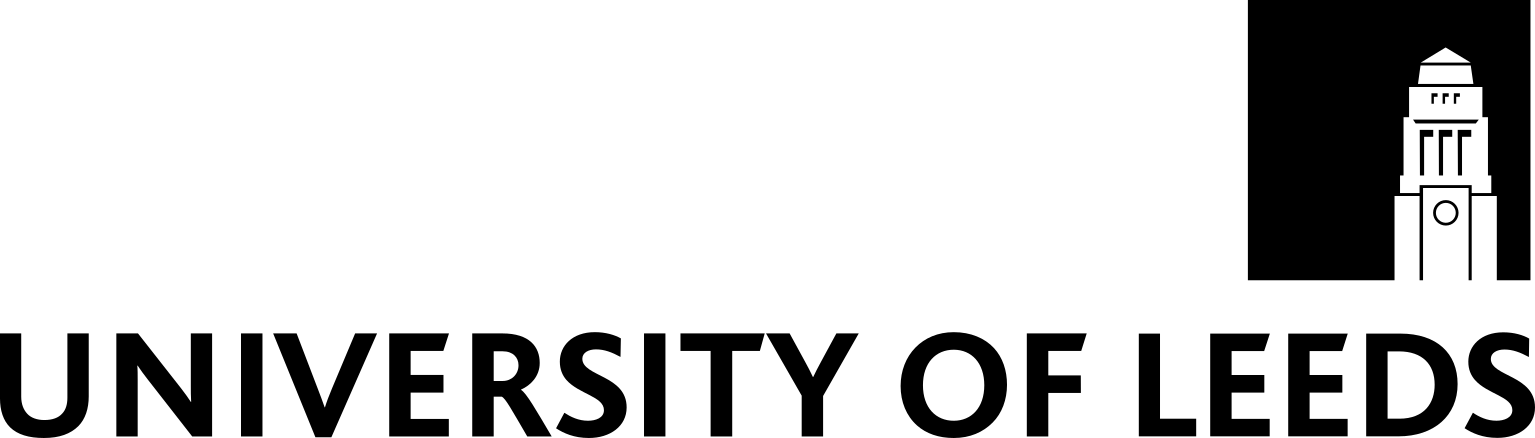
\includegraphics[width=50mm]{UoL_logo}} %University Logo
\deptlogo{} %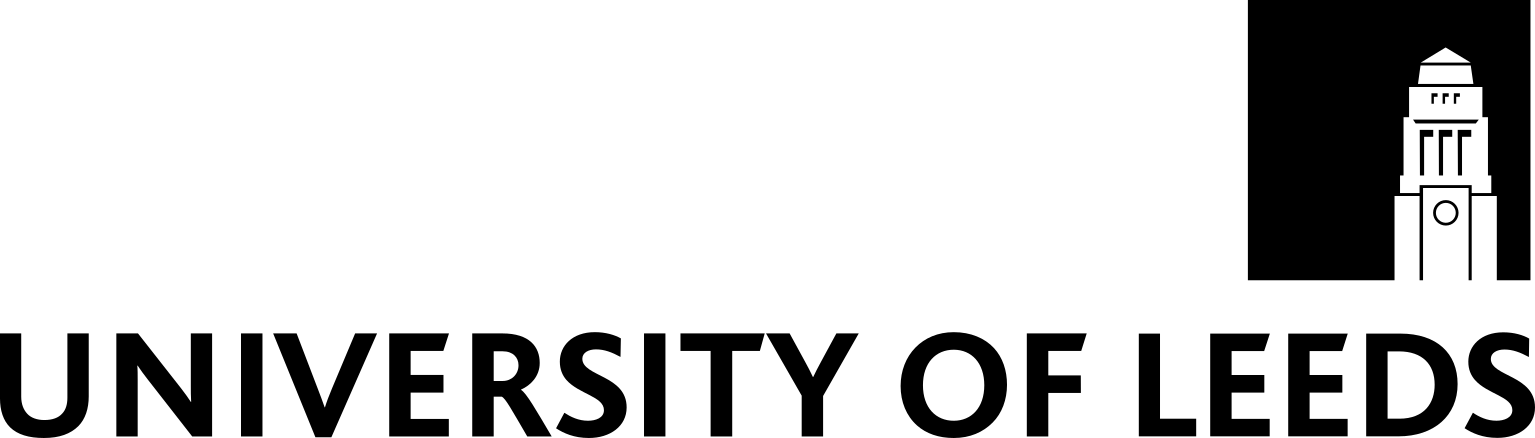
\includegraphics[width=50mm]{UoL_logo}} % Institute Logo
%%%%%%%%%%%%%%%%%%%%%%%%%%%%%%%%%%%%%%%%%%%%%%%%%%%%%%
\collegeordept{\href{https://engineering.leeds.ac.uk/mechanical}{Institute of Design, Robotics and Optimization \\* School of Mechanical Engineering}}
\university{\href{http://www.leeds.ac.uk}{University of Leeds}}

\degree{Doctor of Philosophy}
\degreedate{\monthdate\today}

%Different font in caption
%%%%%%%%%%%%%%%%%%%%%%%%%%%%%%%%%%%%%%%%%%%%%%%%%%%%%%
%%%%%%%%%%%%%%%% Optional Packages  %%%%%%%%%%%%%%%%%%%%%%%%%%%
%%%%%%%%%%%%%%%%%%%%%%%%%%%%%%%%%%%%%%%%%%%%%%%%%%%%%%
%\usepackage{StyleFiles/watermark}
\usepackage{xspace}  %add a space after maths if not already there
%\usepackage{booktabs} %better tables
%\usepackage{rotating}  %rotating figures and tables
\usepackage{array} %enhanced tables
%\usepackage{ctable} %include a figure command
%\usepackage{footnote}
\usepackage{multirow} %for merging cells on tables
%\usepackage{times} % The "Times" font
%\usepackage{Utopia} % The "Utopia" font
\usepackage[toc,page]{appendix}
\usepackage{caption}
\usepackage{subcaption} %This solve the error caused with subfigure
\usepackage{float}
\usepackage{hyperref}
\usepackage{cleveref}
\usepackage[ruled,vlined]{algorithm2e}
\usepackage{enumitem}
\usepackage{rotating}
\usepackage{booktabs}
\newcommand{\ra}[1]{\renewcommand{\arraystretch}{#1}}
%User Definitions
\newcolumntype{C}[1]{>{\centering\arraybackslash}p{#1}}

\linespread{1.3} %1.5 line spacing

\begin{document}

\maketitle

%set the number of sectioning levels that get number and appear in the contents
\setcounter{secnumdepth}{3}
\setcounter{tocdepth}{3}
%Make the label printed by autoref be section for subsection and subsubsection
\let\subsectionautorefname\sectionautorefname
\let\subsubsectionautorefname\sectionautorefname
\pagenumbering{roman}
\frontmatter

%Insert empty page after title
\newpage\null\thispagestyle{empty}\addtocounter{page}{-1}\newpage

%%%%%%%%%%%%%%%%%%%%%%%%%%%%%%%%%%%%%%%%%%%%%%%%%%%%%%
%%%%%%%%%%%% Include sections are required, or comment out to skip over %%%%%%%%%
%%%%%%%%%%%%%%%%%%%%%%%%%%%%%%%%%%%%%%%%%%%%%%%%%%%%%%
%% Thesis Dedictation ---------------------------------------------------

\begin{dedication} %this creates the heading for the dedication page

This thesis is dedicated to someone.

\end{dedication}

% ----------------------------------------------------------------------

%%% Local Variables: 
%%% mode: latex
%%% TeX-master: "../thesis"
%%% End: 

% Thesis IP Statement ---------------------------------------------------

\begin{ipstatement}
The candidate confirms that the work submitted is his own, except where work which has formed part of jointly authored publications has been included. The contribution of the candidate and the other authors to this work has been explicitly indicated below. The candidate confirms that appropriate credit has been given within the thesis where reference has been made to the work of others.
\\
\\
\Cref{sec:chapterDesignGuidelines} of this thesis is based on a jointly-authored conference paper: \textit{Solis-Ortega, R.D., Dehghani-Sanij, A.A. and Martinez-Hernandez, U., 2017, July. Characterization of kinetic and kinematic parameters for wearable robotics. In Annual Conference Towards Autonomous Robotic Systems (pp. 548-556). Springer, Cham.}.
\\
\\
\Cref{sec:ChapterModellingLVM} of this thesis is based on a jointly-authored conference paper: \textit{Solis-Ortega, R.D., Dehghani-Sanij, A.A. and Martinez-Hernandez, U., 2018, August. The assessment of viscoelastic models for non-linear soft materials. In 2018 7th IEEE International Conference on Biomedical Robotics and Biomechatronics (Biorob) (pp. 1274-1279). IEEE.}.
\\
\\
The contributions of the candidate to these papers include the literature review, data collection, design and execution of simulation, statistical analysis, and writing. The contributions of the other authors to these papers include guidance, supervision, and revision.
\\
\\
This copy has been supplied on the understanding that it is copyright material and that no quotation from the thesis may be published without proper acknowledgement.
\\
\\
The right of \theAuthor{} to be identified as Author of this work has been asserted by him in accordance with the Copyright, Designs and Patents Act 1988.
\\
\\
\copyright{} \yeardate{\today} The University of Leeds and \theAuthor{}.

\label{ips}
\end{ipstatement}

% ----------------------------------------------------------------------

%%% Local Variables: 
%%% mode: latex
%%% TeX-master: "../thesis"
%%% End: 

% Thesis Acknowledgements ------------------------------------------------


%\begin{acknowledgementslong} %uncommenting this line, gives a different acknowledgements heading
\begin{acknowledgements}      %this creates the heading for the acknowlegments

\setlength{\parindent}{17.62482pt}
\setlength{\parskip}{0.0pt plus 1.0pt}

\textit{I would like to thank to both Professor Abbas Dehghani-Sanji and Dr Uriel Martinez Hernandez who have guided me on the pursue of a PhD. As well as the many people who directly or indirectly were involved in this personal goal. I would like to thank my family for always being extremely supporting and to my financial sponsor, CONACYT.}

\end{acknowledgements}
%\end{acknowledgmentslong}

% ------------------------------------------------------------------------

%%% Local Variables: 
%%% mode: latex
%%% TeX-master: "../thesis"
%%% End: 


% Thesis Abstract -----------------------------------------------------


%\begin{abstractslong}    %uncommenting this line, gives a different abstract heading
\begin{abstracts}        %this creates the heading for the abstract page

%\setlength{\parindent}{17.62482pt}
%\setlength{\parskip}{0.0pt plus 1.0pt}

Recently, the implementation of the viscoelastic properties found in the human skeletal muscle system is being done for soft robotic applications. Reliable modelling tools capable of predicting this viscoelasticity are required. Therefore, the aim of this research is to systematically compare the performance of two main modelling approaches which are model-based, and data-driven based. Specifically, the performance of these approached when being implemented as part of a control system to predict the mechanical behaviour of viscoelastic materials, is of interest. For this, seven different elastomers were studied. On the model-driven side, the piecewise linearization (PL) method was applied to the Standard Linear Solid (SLS) model and the Wiechert model. On the data-driven side, a feedforward artificial neural network (ANN) was developed. The viscoelastic properties of the selected materials were extracted using the mechanical tests of tensile strength and stress relaxation. The developed models are desired to account for the nonlinear, strain-dependent, and time-dependent stress response of the materials, with the aim of being deployed as part of a control system.

The findings of the research are as follows. On the model-driven side, only one of the two developed models delivered adequate results, the PL-SLS model. The trade-of between complexity and accuracy of this model was characterized. Nonetheless, it was unable to account for time-dependant properties. On the data-driven side, the developed ANN model was able to account for both strain-dependent and time-dependent properties when being assessed in a steady-state environment. However, the validation of the ANN model during real-time predictions was unsatisfactory. The ANN model does not perform well when the strain rate in its input is varying over time. Nonetheless, when the strain rate is fixed, the ANN model is able to follow any type of strain input signal. Lastly, the design of a bio-inspired series-elastic actuator is conceptualized. The intended application for this is to assist the knee joint during walking activities. The experimental protocol designed to test concepts such as co-contraction and variable recruitment is presented as well. The development of the designed actuator was not possible due to time restriction. Nonetheless, all the information regarding the design process is provided in this work.

%The best ANNs candidates were selected based on three main aspects: performance (mse) during train, validation and test, $R^2$ values across all different strain rates, and performance (mse) when presenting the ANNs with unknown experimental data. Subsequently, their real-time prediction was assessed and compared, against the PL-SLS model, in Simulink. In conclusion, this research presents a detailed description on the design, development and implementation of model-driven and data-driven approaches for the prediction of the viscoelastic mechanical behaviour of soft materials, and assess the performance of these approaches when being implemented as part of a control system in a robotic application.

\end{abstracts}
%\end{abstractslong}

% ----------------------------------------------------------------------

%%% Local Variables: 
%%% mode: latex
%%% TeX-master: "../thesis"
%%% End: 

\tableofcontents
\listoffigures
\let\cleardoublepage\clearpage
\listoftables
\begin{abbreviations}
%Place your abbreviations in here...

% Table generated by Excel2LaTeX from sheet 'abbr'

\begin{table}[h]
\centering
\footnotesize{
\begin{tabular}{lp{5cm}lp{5cm}ll}
ADL     & Activities of Daily Living &      NatPolR & Natural Rubber with Polyester \\
ANN     & Artificial Neural Network &      NMAD    & Normalized Mean Absolute Difference  \\
ASTM    & American Society for Testing and Materials &      NR      & Nitrile Rubber  \\
BR      & Bayesian Regularization &       NRMSE   & Normalized Root Mean Square Error  \\
CE      & Contractile Element &     PAM     & Pneumatic Artificial Muscle  \\
CAM     & Computer Assisted Manufacturing &      PE      & Passive Element  \\      
EPR     & Ethylene Polypropylene rubber &      PL      & Piecewise Linearization  \\
FEA     & Finite Element Analysis & PHRI    & Physical Human-Robot Interaction \\      
FFNN    & Feedforwad Artificial Neural Network & PR      & Polyethylene Rubber  \\
FFRD    & Feedforwad Rate-dependent & RMSE    & Root Mean Square Error  \\       
FR      & Fluorocarbon Rubber & SE      & Series Element \\     
FFRI    & Feedforwad Rate-independent & SDS     & Strain-dependent Stiffness \\     
HMS     & Human Musculoskeletal System &     SEA     & Series-elastic Actuator \\    
IMU     & Inertial Measurement Unit &      SLS     & Standard Linear Solid \\
IPAM    & Inverse Pneumatic Artificial Muscle &      SMA     & Shape Memory Alloy  \\
KKP     & Kinetic and Kinematic Parameters &      SMP     & Shape Memory Polymer\\  
LDA     & Large Deformation Actuators &      SSE     & Sum of Square Errors  \\      
LM      & Levenberg-Marquardt &      SR      & Silicon rubber  \\     
LVM     & Linear Viscoelastic Model &      SVA     & Series-viscoelastic Actuator  \\
MAD     & Mean Absolute Difference & TSSE    & Total Sum of Square Errors \\
MSE     & Mean Square Error & TPE     & Thermoplastic Elastomer  \\
NLS     & Non-linear Spring & TPU     & Thermoplastic Polyurethane  \\
NatR    & Natural Rubber \\


\end{tabular}
}
\label{tbl:Abbreviations}
\end{table}

%\begin{table}[here]
%\centering
%\begin{tabular}{ll}
%
%2DEG & Two Dimensional Electron Gas\\
%AC & Alternating Current\\
%AR & Andreev Reflection \\
%BCS & Bardeen-Cooper-Schrieffer\\
%BLG & Bi-Layer Graphene\\
%CCD & Charge Coupled Device \\
%CNP & Charge Neutrality Point\\
%CVD & Chemical Vapour Deposition\\
%DAC & Digital-to-Analogue Converter\\
%DC & Direct Current\\
%DFT & Density Functional Theory \\
%EBL & Electron Beam Lithography\\
%EFE & Electric Field Effect\\
%FET & Field Effect Transistor\\
%FLG & Few Layer Graphene\\
%FWHM & Full Width Half Maximum\\
%h-BN & hexagonal Boron Nitride\\
%IPA & Isopropyl Alcohol \\
%JJ & Josephson Junction\\
%MAR & Multiple Andreev Reflections\\
%MIBK & Methyl Isobutyl Ketone\\
%MR & Magnetoresistance\\
%OL & Optical Lithography \\
%PMMA & Poly(Methyl Meth-Acrylate)\\
%QHE & Quantum Hall Effect\\
%SdHO & Shubnikov de-Haas Oscillation\\
%SEM & Scanning Electron Microscope\\
%SGS & Superconductor-Graphene-Superconductor\\
%SIS & Superconductor-Insulator-Superconductor\\
%SLG & Single Layer Graphene\\
%SNS & Superconductor-Normal-Superconductor\\
%SPCM & Scanning Photo-Current Microscopy\\
%TK & Tuinstra-Koenig\\
%TLM & Transfer Length Measurement\\
%UHV & Ultra High Vacuum\\
%VTI & Variable Temperature Insert\\
%
%\end{tabular} 
%\label{tbl:Abbreviations}
%\end{table}

%$V_{D}$ & Dirac Point voltage \\
%$V_{g}$  & Gate voltage\\
%$E_{F}$ & Fermi Energy\\
%$v_{f}$ & Fermi velocity \\
%$\omega_{c}$ & Cyclotron Frequency \\
%%$k_{B}$  & Boltzmann's constant \\
%T_{c}

\end{abbreviations}

\begin{Common_Symbols}
%Place your abbreviations in here...

% Table generated by Excel2LaTeX from sheet 'abbr'

\begin{table}[h]
\centering

\begin{tabular}{ll}

$\lambda$   & Extension Ratio \\
$\varepsilon$   & Strain \\
$\varepsilon_o$   & Initial Strain \\
$\varepsilon_{u}$   & Ultimate Strain \\
$\varepsilon_{ue}$   & Engineering Ultimate Strain \\
$\varepsilon_{y}$   & Yield Strain \\
$\sigma$   & Stress \\
$\sigma_o$   & Initial Stress \\
$\sigma_{u}$   & Ultimate Stress \\
$\sigma_{ue}$   & Engineering Ultimate Stress \\
$\sigma_{y}$   & Yield Stress \\
$\sigma_{end}$   & Final Stress \\
$A_o$   & Cross-sectional Area \\
$l_o$   & Initial Length \\
$\Delta L$ & Elongation \\
$\Delta L_o$ & Initial Elongation \\
$F$     & Force \\
$k$     & Spring constant \\
$k_e$     & Equilibrium Spring constant \\
$k^*$     & Strain-dependent Spring \\
$\eta$     & Damper Constant \\
$E$     & Elastic Modulus \\
$E_{small}$     & Elastic Modulus at Small Strains\\
$E_{large}$     & Elastic Modulus at Large Strains\\
$\varepsilon_{offset}$ & Strain Offset \\
$S.R.$      & Stress Relaxation\\
$R^2$      & Coefficient of Determination\\

\end{tabular}

\label{tbl:Common_Symbols}
\end{table}

%\begin{table}[here]
%\centering
%\begin{tabular}{ll}
%
%2DEG & Two Dimensional Electron Gas\\
%AC & Alternating Current\\
%AR & Andreev Reflection \\
%BCS & Bardeen-Cooper-Schrieffer\\
%BLG & Bi-Layer Graphene\\
%CCD & Charge Coupled Device \\
%CNP & Charge Neutrality Point\\
%CVD & Chemical Vapour Deposition\\
%DAC & Digital-to-Analogue Converter\\
%DC & Direct Current\\
%DFT & Density Functional Theory \\
%EBL & Electron Beam Lithography\\
%EFE & Electric Field Effect\\
%FET & Field Effect Transistor\\
%FLG & Few Layer Graphene\\
%FWHM & Full Width Half Maximum\\
%h-BN & hexagonal Boron Nitride\\
%IPA & Isopropyl Alcohol \\
%\Vg & Gate Voltage \\
%JJ & Josephson Junction\\
%MAR & Multiple Andreev Reflections\\
%MIBK & Methyl Isobutyl Ketone\\
%MR & Magnetoresistance\\
%OL & Optical Lithography \\
%PMMA & Poly(Methyl Meth-Acrylate)\\
%QHE & Quantum Hall Effect\\
%SdHO & Shubnikov de-Haas Oscillation\\
%SEM & Scanning Electron Microscope\\
%SGS & Superconductor-Graphene-Superconductor\\
%SIS & Superconductor-Insulator-Superconductor\\
%SLG & Single Layer Graphene\\
%SNS & Superconductor-Normal-Superconductor\\
%SPCM & Scanning Photo-Current Microscopy\\
%TK & Tuinstra-Koenig\\
%TLM & Transfer Length Measurement\\
%UHV & Ultra High Vacuum\\
%VTI & Variable Temperature Insert\\
%
%\end{tabular} 
%\label{tbl:Abbreviations}
%\end{table}

%$V_{D}$ & Dirac Point voltage \\
%$V_{g}$  & Gate voltage\\
%$E_{F}$ & Fermi Energy\\
%$v_{f}$ & Fermi velocity \\
%$\omega_{c}$ & Cyclotron Frequency \\
%%$k_{B}$  & Boltzmann's constant \\
%T_{c}

\end{Common_Symbols}


\mainmatter

\pagenumbering{arabic}
\chapter{Introduction} \label(ch1:introduction)
\section{ Background}

The field of Soft robotics deals with the implementation of soft and deformable materials in traditional Robotics applications. The interest and research in this field has increased in the past decade. The latter is due to the outstanding developments in terms of manufacturing of soft materials, such as elastomers, and the development of new soft materials which can be stimulated, i.e. deformed, by heat, light, and magnetism. 

The coordination action called RoboSoft, supported by the IEEE Robotics and Automation Society (RAS) and the European Commission, has played a very important role in spreading the awareness of the wide number of Soft Robotics applications. The RoboSoft committee formally defines the field of Soft Robotics as ``Soft robot/devices that can actively interact with the environment and can undergo `large' deformations relying on inherent or structural compliance'' \cite{laschi2016soft}. The categorization of when a robotic application fall into the field of Soft Robotics depends on the material's Young Modulus, a mechanical property which relates the material's deformation with the amount of stress applied to it; which must be between the range of 10$^{2} - $10$^{6}$ Pascals (Pa). The Young's modulus is usually a measure of a solid material stiffness; a high value refers to a stiff material in the same way as a low value refers to an elastic or soft material. In the context of Soft Robotics, the term compliance it is most used instead of stiffness since it refers to the adaptability of the material under certain circumstances.

Early applications in Soft Robotics were inspired in nature, by observing that most biological organisms are not rigid, e.g. the human skeleton only contributes with 11\% of an adult's weight, on contrast, the skeletal muscle in our body only contributes with 42\% of the weight \cite{kim2013soft}. This inspiration gave birth to several soft bio-inspired robots, as well as the interest in studying the embodied intelligence of biological organisms. The latter refers to the ability of biological organisms to adapt to different situations by exploding their body morphology and properties. This is one of the main differences between soft and rigid robots. The embodied intelligence of soft robots release the controller from the task of accurately controlling the position of the robot and of constantly monitoring the working environment; allowing the controller to focus on the execution of commands. This is only possible with the implementation of soft and deformable materials able to automatically adapt to perturbations from the environment, such as uneven terrains and obstacles. Bio-inspired soft robots are now being developed for a broad range of applications, such as locomotion, manipulation, and even replicating biological processes such as digestion. The research done in the field of Soft Robotics has an interesting multidisciplinary potential. For example, the locomotion of caterpillars and snake could be study by building a soft robot which replicates this motion. The knowledge extracted from this could be useful for the development of actuated bendable soft cylinders which ultimately could replace the current rigid tools being used in laparoscopic surgery \cite{rus2015design}.

The mechanical behaviour of soft materials, is very difficult to model using traditional mathematical models, due to their non-linear, time-dependent and strain-rate-dependent stress response. This great challenge motivated the research in Soft Robotics to develop bio-inspired soft bodies, arms and legs able to perform the task at hand using minimal control. This caused a shift in the traditional design approach for rigid robots from ``rigidity by design, safety by sensors and control'' to design approach used in soft robots, ``safety by design, performance by control''. The added feature of safety, inherent in most soft robots, allowed the development of Physical Human-Robot Interaction (PHRI) applications \cite{filippini2008toward}. Many other challenges face by this emerging field are listed in \cite{laschi2016soft,trivedi2008soft} being: actuation of soft materials, development and implementation of soft sensors into soft robots, control systems able to deal with the nonlinear behaviour of soft materials, and modelling tools able to accurately predict the mechanical behaviour of soft materials in real-time. Most of these limitations come from the simple fact that soft robots cannot be considered as a chain of rigid links able to rotate or slide as common robots are, but soft robots are deformable and continuous which means that all the foundation in which Robotics is based on, is not easily transferable to the Soft Robotics field. 

The design and development of soft robots is very challenging, however, the potential benefits are many \cite{iida2011soft}. Foe example, soft robots have the potential of being very dexterous due to the ability of modifying their shape depending on the environment; soft robots can can manipulate objects of different shapes, sizes, and most importantly they are safe to interact with humans in the event of an unplanned collision. The latter benefits highlight the potential of Soft Robotics for PHRI applications such as, orthoses, surgical tools, and wearable devices. This research aims to contribute to the technological advance of Soft Robotics for human assistance applications.

For a long time, humans have pursued the idea of increasing their strength, stamina and speed through different means. Currently, we are relaying on technological advances to achieve the latter by building wearable robotic devices, commonly known as robotic exoskeletons. This wearable device was motivated by military applications where a soldier is required to carry a heavy load in its back for a long period of time, ultimately causing him injuries or early fatigue. The robotic exoskeleton is able to carry a payload and transmit the payload weight to the ground, ideally relieving the wearer from feeling the payload, which allows the wearer to walk greater distances without premature fatigue. The rigid nature of these devices and the big actuators implemented to achieve forces able to enhance humans, impose many limitations, such as, restriction of body movements, interference on subject natural biomechanics and high inertia which impedes the device to follow the subject intentions smoothly, creating a drag feeling \cite{asbeck2014stronger}.

In the field of Soft Robotics, research is being done to develop a soft version of a robotic exoskeleton, formally called soft exosuit, in an attempt to solve the previously mentioned limitations. Soft exosuits are wearable robotic systems meant to be worn in the same way as clothes, by attaching both the actuation and perception systems into a wearable structure, made of textiles, strapped to the human body which will ultimately assist the wearer's motions. Despite the many benefits of this technology, in comparison to the robotic exoskeleton, current developments of soft exosuits are not able to deliver enough mechanical power to be called an enhancement device. Currently, soft exosuits are considered an assistive device. This limitation is inherent from the idea of having a soft wearable device. The conversion of forces and torques, generated by the actuators attached to a wearable textile or directly to the user's body, into useful assistive torques for human joints assistance is very challenging. In a rigid exoskeleton the reaction forces produced by the actuators are sustained by the exoskeleton mechanical frame, but this is not the case in soft exosuits, where the reaction forces must be dissipated through the worn textile attached to the human body, which generates uncomfortable frictions between the user skin and the textile. Nevertheless, the human body naturally possesses areas able to sustain high amounts of forces, these areas are currently being exploited into soft exosuit designs to prevent discomfort, skin injury, and to increase the efficiency of transmitted forces. The latter principle is implemented in \cite{wehner2013lightweight} where a lower limb soft exosuit using pneumatic muscles is developed. The other, most common approach is to fix a wearable soft material to the skin, as in \cite{park2014design,park2011bio} where pneumatic artificial muscles (PAM) were attached to a soft cloth and disposed in such a way that they can mimic the biological musculoskeletal behaviour of a human foot. Among the available soft exosuit developments, few of them implements a closed loop control system, due to the high complexity of dealing with the non-linearity of soft materials. 

%On the other hand, several works focus on the characterization and testing of soft technologies as \cite{wehner2012exp} where an accurate characterization of a PAM is performed, which directly contribute to the development of previously mentioned soft exosuits. Many other technologies are being researched as well, such as, shape memory alloys (SMAs), which are metal alloys capable of changing its form when  properly stimulated. One of the main drawbacks of this technology is the amount of energy and time required to heat metal alloy and activate its shape shifting ability. The latter limitation is highlighted in \cite{Stirling2011}, where soft orthoses for foot and knee were developed SMA springs embedded in a soft fabric. The response of the device was to slow to be used for human assistance. Another commonly implemented actuation technology are cable-driven actuators, typically consisting of an electric motor and a Bowden cable. This electromechanical system create pulling forces by applying tension to a cable fixed in two different points. The cables must be routed along the body of the wearer to deliver the acting force to the joint of interest \cite{asbeck2013biologically,asbeck2015biologically}. The stroke length is not limited in this type of technology, as is the case for PAMs, since Bowden cables are flexible and can be routed in many different ways.

%Many soft sensing technologies have also been developed, being hyper-elastic strain sensors the most common one, which are based on the change in resistance of a liquid metal alloy inside conducts embedded into an elastic polymer which allows the measurement of the body limb position and sustained forces; its performance allowed the development of a soft artificial skin \cite{park2012design}. This technology was later implemented in a soft exosuit to allow for the measurement of the human biomechanics. A comparison analysis between the latter approach and the well-established motion capture technology was performed in \cite{mengucc2014wearable}, where the implementation of strain sensors to capture the human biomechanics showed remarkable results.

The progress in the field of Soft Robotics has been very quick and very diverse. Most of the research is focused on studying the benefits of using a specific new soft material in a robotic application, leaving the control system on a second plane. This is mostly due to the complexity of developing a modelling tool to accurately predict the mechanical behaviour of soft materials. As previously mentioned, this is one of the main challenges in Soft Robotics applications and the main focus of this research.

In the literature, most of the works are based on one of two approaches, either a model-driven approach or a data-driven approach. On one hand, the model-driven approach, as suggested, is based on using mathematical models to predict the mechanical behaviour of soft materials. Due to the time-dependent properties, or viscoelasticity, exhibited in most soft materials, model-driven approaches use a set of equations for model viscoelasticity known as the Linear Viscoelastic Models (LMV). These models describe a material using two basic mechanical components, a spring and a dashpot, arranged in different configurations. Inside this group, there are two models which can be expanded as required. In theory, this means these two models could be able to describe the most complex soft material as long as enough they are expanded as required. In practice, expanding a mathematical model is translating into solving more equations at a given time, and this is translated into demanding more computational power. Therefore, the model-driven approach has a well-known trade-off between achievable accuracy and required computational power, making the deployment of control systems based on this approach prohibitive. 

On the other hand, the data-driven approach is based on machine learning tools, specifically Artificial Neural Networks (ANNs). The implementation of this tools for the prediction of the mechanical behaviour of viscoelastic materials has been researched for more than a decade, showing very good performance. ANNs are very good at identifying patterns inside complex data. The training process is known to take plenty of time, depending on the complexity and amount of data. However, once the ANN is trained, they are able to receive an input and produce an output almost immediately. This is the main advantage of ANNs in comparison to model-driven approaches, which have to perform intensive calculations every time new data is presented as input.

As the field of machine learning advances, better tools are becoming available, which leaves room for performing optimizations on previous works and on assessing new machine learning algorithms. At the time of starting this research and at the best of my knowledge, there was no documented work assessing the performance of ANNs as an alternative to model-driven approach when being deployed as part of a control system for a robotic application. In other words, the real-time prediction performance of neural network was not being assessed. Therefore, this research aims to fill this gap in the knowledge.

\section{Motivation}

The global percentage of elderly population is constantly rising. The World Health Organization has estimated that the global percentage of people aged 65 or older will triple by 2050, with respect to 2010 \cite{Colombo2012}. Moreover, the amount of elderly people living alone is also increasing. Solely in the United Kingdom, there are 1 million people aged over 65 living on their own \cite{Hill2019}. Although, the social triggers of the mentioned phenomenons are out of the scope of this research, they represent a strong motivation to push forward the research on Soft Robotics applications for human assistance. Currently, there are viable concepts of assistive exosuits targeted to increase the quality of life of elderly people during activities of daily living, such as walking over ground, ascending stairs, using a chair. However, the concept of an assistive exosuit is relatively new, the first documented prototype is dated from 2013 \cite{wehner2013lightweight}. The idea behind an exosuit is to translate the proven concept of a robotic exoskeleton, which is a heavy and bulky wearable device aimed to enhance the strength of humans, into a soft, light weight and compliance version aimed to provide assistance to the elderly or disabled people. 

One of the main challenges in this field of research is the modelling of the mechanical behaviour of soft materials. The accuracy of current modelling approaches is restricted by the computational cost required. This prevent them to be deployed in most micro-controllers, due to the limited computational power available in this devices. Commercially ready exosuits might be possible in a decade time, meanwhile there is plenty of research to be done to translate well developed technologies used in Robotics into the field of Soft Robotics. Summarizing, this research can improve the quality of life of the elderly and disabled population by developing a novel modelling approach which will enable current soft actuation technologies to be more reliable when being implemented in soft exosuits.

\newpage

\section{Aims and Objectives}

\subsection{Aims}

The aims of this research are:

\begin{itemize}
    \item To investigate the concept of mimicking the viscoelastic mechanical properties of the human musculoskeletal system in Soft Robotics applications for human assistance of the lower limb.
    \item To identify and assess the most commonly used modelling approach for the prediction of viscoelastic stress response of soft materials.
    \item To assess the performance of the modelling approach when being implemented as part of a control system for the real-time prediction of the stress response of a material, in a simulation environment.
\end{itemize}

\subsection{Objectives}

In accordance to the research aims, the following objectives are identified:

\begin{itemize}
    \item Perform a literature review of the following topics:
    \begin{itemize}
        \item The biomechanics of the human the lower limb during activities of daily living.
        \item Soft Robotics applications for human assistance of the lower limb.
        \item Soft actuation technologies currently used for the assistance of the human knee joint.
        \item Modelling techniques being used for the prediction of the stress response of viscoelastic soft materials.
    \end{itemize}
    \item Compile a database for the human lower limb biomechanics during activities of daily living, such as: walking, ascending/descending stairs, ascending/descending ramps and sitting down/standing up from chair.
    \item Characterize the viscoelastic mechanical behaviour of suitable soft materials.
    \item Compare the mechanical properties of these materials against the mechanical properties of the human tendons involved in the motion of the knee joint.
    \item Identify the techniques being used for the modelling of the viscoelastic behaviour of soft materials, in applications for human assistance.
    \item Develop a better modelling approach, or optimize current ones, to allow the accurate prediction of the viscoelastic stress response of soft materials.
    \item Assess the performance of the latter modelling approach.
    \item Assess the prediction accuracy of the mentioned modelling approach:
    \begin{itemize}
        \item Design a simulation environment based on a known soft actuator controlling a load.
        \item Establish the control system target based on the torque-speed requirements of the knee joint.
        \item Assess the compatibility of the modelling approach when being implemented as part of the mentioned control system for the real-time prediction of the stress response of a soft material.
    \end{itemize}
\end{itemize}

\section{Scope of the research}

This research is focused on developing a reliable modelling tool, able to be implemented in a control systems, for the prediction of the mechanical behaviour of soft materials. Therefore, the following is included in the scope of the research. 

The biomechanics from the lower limb of the human body during several activities of daily living are characterized. The potential benefits of using a viscoelastic material instead of the traditional metallic spring in series-elastic actuators, is investigated. For this reason, the following soft materials are studied: ethylene polypropylene rubber (EPR), fluorocarbon rubber (FR), nitrile rubber (NR), natural rubber with polyester(NatR),  polyethylene  rubber  (PR),  silicone  rubber  (SR), and  100\% natural rubber (NatR100). A recent and accurate model-drive approach, based on a piecewise linearization of the Linear Viscoelastic Models (LMVs) is studied. Furthermore, a systematic analysis on the performance of a popular data-driven approach, Artificial Neural Networks (ANNs) is executed. The analysis includes the effect on the number of neurons, output activation function, training algorithm, and combination of inputs/outputs presented to the network. Moreover, a comparison analysis on the performance of these approaches when being implemented as part of a bio-inspired series-elastic actuator model, in a control system, is assessed. The control system requirements are designed to meet the knee joint torque-speed characteristics, previously characterized, during level ground walking. Finally, the most suitable modelling approach for this application is identified.

\section{Contributions of the research}

The research contributes to the field of Soft Robotics for human assistance by investigating the performance of Artificial Neural Networks, as an alternative to the Linear Viscoelastic Models, for the modelling of viscoelasticity in soft materials. Some parts of this thesis are published in peer-reviewed conference papers. The contributions are summarized as follows:

\begin{itemize}
    \item Assessment of relationship between the accuracy and the mathematical complexity, of the Piecewise Linearized Standard Linear Solid model.
    \item Development of a model-driven modelling approach, based on the piecewise linearization method, applied to one of the most complete LMVs, the Wievhert model.
    \item Development of a data-driven approach, based on ANNs, for the prediction of the mechanical behaviour of soft materials.
    \item Development of a bio-inspired series-elastic actuator model, which use the data-driven modelling approach to predict the mechanical behaviour of the soft elastic element in the actuator.
\end{itemize}

\section{Outline of the thesis}

This thesis divided and organized in six chapters, as follows:
\begin{itemize}
    \item {\bf Chapter 1: } This chapter presents the research background, motivation of the researcher, aims and objectives. Moreover, the specific contributions of this research to the respective field of knowledge, and the scope of the thesis is also presented in here.
    \item {\bf Chapter 2:} The second chapter describes the state of the art on soft robotics applied to human assistance. The latter is organized in three main sections: soft actuation technologies, soft perception systems and soft robotics controllers. However, the main focus of this chapter is directed to innovative soft actuation technologies by describing their advantages, limitations and possible solutions. Furthermore, the design aspects of the soft orthoses and soft exosuits analysed for the realization of this chapter are also described. The design approach of mimicking the human musculoskeletal functionality is also described in here. The terminology related to human biomechanics, and characterize the torque, speed, and angle of motion, of the human lower limb (hip, knee, ankle) during activities of daily living (ADL). A total of four main ADL are investigated from clinical trials: ground level walking, going up/down steps, going up/down a ramp and sitting down/standing up from a chair.The compiled data is post-processed to obtain a graphical representation and facilitate the comparison and analysis of the parameters variations from subject to subject and activity to activity. Finally, this literature review highlighted the research opportunities of implementing a soft material as the elastic element of traditional series-elastic actuators, replacing the commonly used metallic spring. To do this, a reliable modelling tool, able to predict the mechanical behaviour of soft materials, must be developed.
    \item {\bf Chapter 3: } This chapter explains the preliminary experimental work performed with the aim of finding a soft material able to replicate as close as possible the mechanical properties of the human tendon. The latter is motivated by the commonly practice of assuming a perfectly stiff tendon when implemented the mechanical model of the human muscle-tendon system in soft orthoses. Seven different elastomers are selected as possible candidates. The mechanical properties of these materials are extracted using the tensile strength test and the stress relaxation test. Subsequently, the data is post-processed and compared with the properties found in human tendons to identify the most suitable material to be used in a soft series-elastic actuator.
    \item {\bf Chapter 4: } This chapter describes the assessment performed to a modelling tool based on the Standard Linear Solid model, which is modified to account for strain-dependent stress response in elastomers by applying a piecewise linearization to the mentioned model
    \item {\bf Chapter 5: } The fifth chapter presents the achieved conclusions, future work and proposed research plan.
    \item {\bf Chapter 6: }
\end{itemize} %% file path for chapter tex files 
\newpage\null\thispagestyle{plain}\newpage
\chapter{Literature Review}

\section{Introduction}

This chapter presents the performed literature review about soft robotic applications implemented in human assistance, such as soft exosuits and soft orthoses. The chapter is organized to individually present three main aspects of current soft robotic applications: the soft actuation system, the soft perception system, and the control system. In addition to this, the design process involved in developing soft wearable suits, as part of each soft robotic application, is described. Following the latter, the identified gaps in the body of knowledge are presented. Lastly, the relevant findings of the performed literature review are summarized in the last section of this chapter.

\section{Soft Robotics for Human Assistance Applications}

The adoption of soft robotics in human assistance applications was slowly approached by replacing the rigid and bulky actuators of traditional robotic exoskeletons with soft actuators such as Pneumatic Artificial Muscles (PAMs) and Bowden cables. The latter gave birth to hybrid systems as found in \cite{Noda2014}, where a combination of both the previously mentioned technologies were implemented to overcome the high inertia limitation present in robotic exoskeletons. Furthermore, the latter paper presents the first attempt, unintentionally, to imitate the functionality of the human musculoskeletal system by using Bowden cables to transmit the forces created by the PMAs in a similar muscle-tendon behaviour. 

During the following years of this transition many rigid devices were implementing soft actuators motivated by the same principle as mentioned earlier. However, in the early stages of soft robotics there was a lack of soft materials able to be implemented as actuators which encouraged researchers to focus mainly on pneumatic actuators \cite{Belforte2014}. As soft robotics gained popularity, researchers in material sciences started to develop new soft materials able to function as actuators. Currently there are many options, some of them still under development, ready to be implemented in different soft robotics applications. Nevertheless, despite the many materials available, current developments in soft exosuits and soft orthoses have focused on two technologies: pneumatic artificial muscles (PAM) and cable-driven actuators, commonly based on electric motors, using Bowden cables as the pulling element. In a lesser quantity, technologies such as shape memory alloys (SMAs) and shape memory polymers (SMPs) have been implemented in soft orthoses with unsuccessful results mainly due to their large recovery time which make them unsuitable for human assistance applications. The extent of how these technologies have been implemented in soft robotic applications is presented in the next subsection.

\subsection{Soft Actuation Technologies} \label{sec:SoftActuation}

\subsubsection{Pneumatic Artificial Muscles} \label{sec:PMAs}

The usage of compressed air or gases into engineering applications is called Pneumatics, if an incompressible fluid is used, it is called Hydraulics; when applied in Soft Robotics, the idea is to expand or contract a soft material mainly to produce forces but it can also be used to produce different types of locomotion in particular soft robots. As previously mentioned, soft pneumatic actuators were extensively researched in different applications for Soft Robotics, in fact, the usage of soft polymers (silicone and elastomers) created the path for several different applications such as legged locomotion \cite{Florez2014}, pneumatic fingers for grasping objects with sensing capabilities \cite{Morrow2015}, soft skin with embedded sensors \cite{Sonar2016,Suh2014} and even implantable cardiac stimulators \cite{Roche2014}. In the area of human assistance, soft pneumatic actuators can be categorized in four main groups: textile muscles, braided fluid muscles (McKibben type), large deformation actuators (LDA) bellows and LDA worm. Only the former three are suitable for some kind of human assistance, however, according to Belforte et al. \cite{Belforte2014}, the most suitable for biomedical application in rehabilitation are the McKibben muscles due to the advantages described in \autoref{tbl:PMAs_feats}.
\begin{table}[htp!]
  \caption{Pneumatic artificial muscles main features. Modified from \cite{Belforte2014}}
  \label{tbl:PMAs_feats}
  \centering
  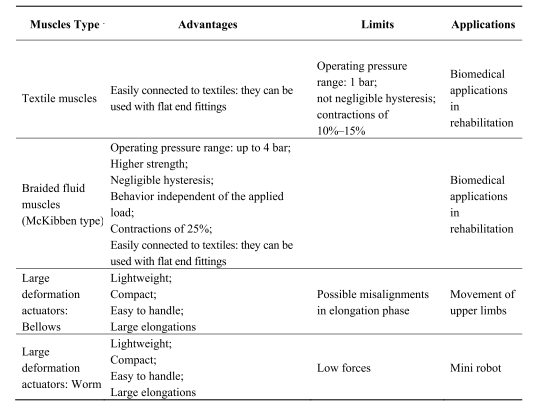
\includegraphics[width=1\textwidth]{Table_PAM_Features.png}
\end{table}

The first works on assistance to human lower limbs using soft robotics \cite{park2011bio,Hamedi2015} describe a soft orthosis for the foot intended to treat gait pathologies, particularly the drop-foot condition. One important aspect of this device is its design, inspired in the musculoskeletal human system, i.e. the actuation system was designed to comply a muscle-tendon-ligament functionality mimicking the natural behaviour of the human body (\autoref{fig:bio_ankle}). The soft orthoses is powered by pneumatic actuators, also called Mckibben-type actuators. They are attached to a soft support structure consisting of an adapted neoprene knee sleeve and a five toed leather shoe. A total of three off-the-shelf pneumatic muscles \autoref{fig:bio_ankle_parts}(a) assisted the dorsiflexion, eversion and inversion movements of the ankle joint by generating tension forces in artificial tendons, made of a flexible but non-extensible metal cable, positioned close to the foot tendons. The tendons were located inside a low friction material tube to prevent generated force losses; two of them were anchored to a single point in the foot brace while the other one was anchored in four different points in order to distribute the pulling force, again, mimicking the human body behaviour. The artificial ligaments provided with the same functionality as the biological ones, which is to restrict the movement of the tendons in all the directions other than the one of actuation (\autoref{fig:bio_ankle_parts}(b)). The pneumatic actuators were strategically anchored in two points, at the bottom of the knee sleeve providing nonrestrictive motion of the knee, and at the foot brace.
\begin{figure}[hbtp!]
    \centering
    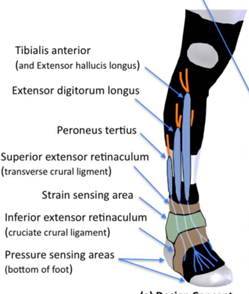
\includegraphics[width=0.4\textwidth]{BioinspiredAnkle.png}
    \caption{Design concept of the bio-inspired active soft orthosis for ankle foot. From top to bottom, the main parts are highlighted: artificial muscles attached to the soft wearable garment, a strain sensor for ankle angle measurements, the tendon-ligament system and pressure sensor for gait cycle detection \cite{park2011bio}. }
    \label{fig:bio_ankle}
\end{figure}
\begin{figure}[hbtp!]
    \centering
    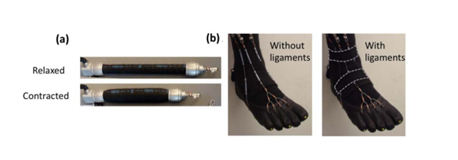
\includegraphics[width=\textwidth]{BioinspiredAnkleParts.png}
    \caption{Some components implemented in the soft orthosis, (a) pneumatic artificial muscle in its relaxed and contracted state and. (b) complete tendon-ligament system without ligaments and with ligaments. \cite{park2011bio}. }
    \label{fig:bio_ankle_parts}
\end{figure}

Another soft orthosis using pneumatic actuation is presented in \cite{Park2012} which extends the concept of embedded sensor and create an embedded sensor-actuator module, which is referred to as a muscle-sensor unit. In order to obtain some degree of compliance with human's lower limb, the device has a cylindrical shape and it is made of a flexible silicone elastomer (EcoFlex 0300). The muscle-sensor units are embedded into the latter shape to form a distributed array of four columns and four rows (16 actuators), allowing the device to have plenty of different motions and delivered torques depending on the number of activated actuators at a given time (\autoref{fig:soft_sleeve}). During the casting process, each column of actuators is tied to each other with Kevlar fibres so they can pull each other when contracting, also the fibres are anchored to both caps of the cylinder in order to achieve the desired movement. When the pneumatic muscle is activated its radius increases and its length decreases, creating a compression force. This design provides some degree of modularity due to the many embedded actuators which can be activated independently. Nevertheless, it has little compliance with the human's lower limb which ultimately complicates the conversion of generated forces into useful torques for assisting the joint of interest.
\begin{figure}[hbtp!]
    \centering
    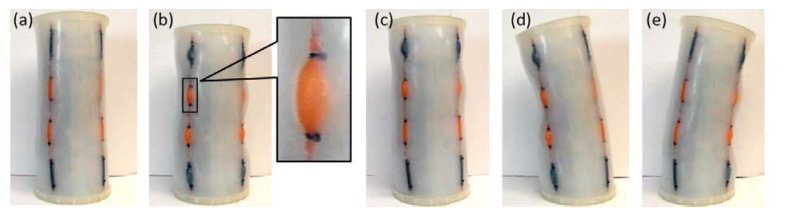
\includegraphics[width=\textwidth]{SoftSleeve.png}
    \caption{Different shapes achieved by the prototype. (a) Original shape. (b) All muscles activated, contracting the whole body and amplified image of one muscle. (c) Partial contraction, only the 1st and 2nd top rows are activated. Both (d) and (e) illustrate bending movements, only two adjacent columns are activated. \cite{Park2012}. }
    \label{fig:soft_sleeve}
\end{figure}

On the other hand, a novel implementation called virtual anchor technique, which used pneumatic artificial muscles, can be seen in \cite{wehner2013lightweight}. Addressing the challenge of force transmission using soft materials attached or strapped to the skin, which for high forces (such as those required in normal walking) will be intolerable for the user, the key anchor points of the human body are defined as the ones exhibiting large bony landmarks. These regions are able to withstand high forces and minimize the slippage or chaffing of soft materials positioning on them. Furthermore, the virtual anchor technique was also motivated by the changes in length of some parts of the skin surface during joint motion in where some parts exhibit more changes than others. Therefore, the soft exosuit was developed by interconnecting PMAs and nylon straps, replicating the extensible and non-extensible paths of the skin, respectively, in the specific points where the changes in the skin length take place, also called virtual anchor points which in combination with the key anchor points allow a good transmission of forces without causing discomfort to the user. In \autoref{fig:anchor_concept} the described concept can be appreciated, the orange lines represent the pneumatic actuators interconnected with the key anchors and the virtual anchors. The latter constrain the actuator's movements other than the desired, as well as redirect the actuator's reaction forces to the body areas able to sustain them. Finally, this design was able to reduce the metabolic cost caused by wearing the complete device of about 10 kg, by almost 100\%. Considering that no control system, other than a timed activation sequence, and no perception system was implemented, this technique opens the door for further improvements to achieve a better degree of assistance.

\begin{figure}[hbtp!]
    \centering
    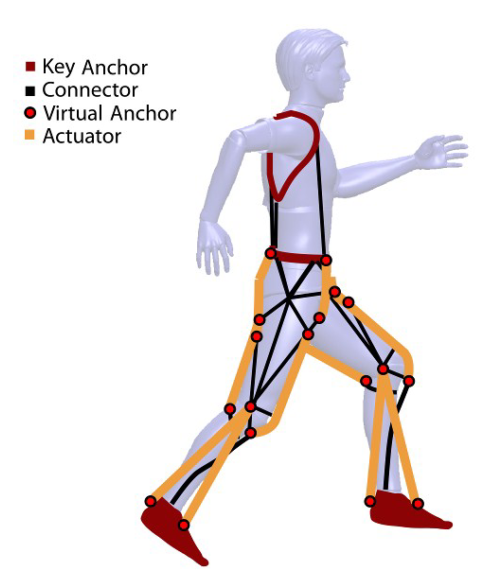
\includegraphics[width=0.45\textwidth]{AnchorConcept.png}
    \caption{Virtual anchor concept. The three key anchors (red square) located at the foot, hip and shoulder are interconnected with the soft actuators (orange) and auxiliary connectors (black) in specific points called virtual anchors (red circle) to stabilize the forces created by the actuators. \cite{wehner2013lightweight}. }
    \label{fig:anchor_concept}
\end{figure}

Putting aside the McKibben-type actuators as the most common choice for pneumatic muscles, elastomers such as high-flexible silicone can be used to build PAM as shown in \cite{Park2014}. This PAM consists of interconnected flat chambers made of silicone rubber which inflate when pressurized air is injected (\autoref{fig:Flat_elastomer}), the innovative concept in this work is the zero-volume air chamber which provides a higher degree of compliance and compactness (traditional PMAs retain air inside them even when they are not actuated). Kevlar fibres are embedded inside this soft actuator to constrain the expansion direction and create a contraction movement when pressurized. The flatness of this actuators simplifies the casting process. Furthermore, the chamber based design make it possible to join each chamber together not only in series, which increases the contraction length, but in parallel as well to increase the contraction force. In order to test the actuator performance, a soft exosuit similar to the previously described was developed using nylon straps and hooks to connect the soft actuator to the points of interest. The developed soft orthosis, intended for infant-toddler rehabilitation, was able to deliver a 38 N contraction force and 18 mm contraction length by implementing a muscle with an array of four elastomer actuators inter-connected in series. In addition, a total excursion for the knee joint of 132\textdegree{} was achieved, considering both flexion and extension motions (\autoref{fig:Flat_elastomer}). Moreover, in a most recent development by \cite{Low2016}, it can be found the implementation of elastomers for ankle assistance, in this case the pulling force of the PAM is generated when the actuator deflates and a pushing force is generated when it inflates, an inverted behaviour in comparison to previously mentioned applications. This soft orthosis consists of a regular sock which is attached to both ends of the PAM, that is enclosed into textile to restrict its longitudinal and radial expansion mainly. Despite the simplicity and assistance capabilities of the device, it can't be worn with shoes, restricting the assistance to indoor activities
\begin{figure}[hbtp!]
    \centering
    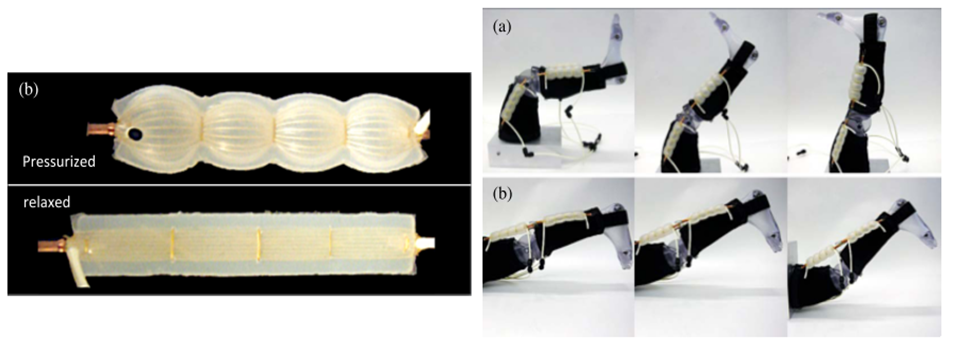
\includegraphics[width=1\textwidth]{FlatElastomer.png}
    \caption{(a) Flat elastomer pneumatic actuator in its both (1) pressurized and (2) relaxed states. (b) Implementation of the flat actuator in medical leg model assistance, along with the achieved extension (1) and flexion (2) motion. \cite{Park2014} }
    \label{fig:Flat_elastomer}
\end{figure}

This concept of expanding, instead of contracting, the PAM when pressurizing is called Inverse PAM (IPAM). This very recent type soft actuator, called `Hydro Muscle', is directly compared with McKibben muscles since it overcomes the main limitations of the latter. The main difference between this actuator and the previously mentioned is the shift from pneumatic technology to hydraulics, in fact, it is reported that the pressure found in homes tap water is enough to actuate it \cite{Sridar2016}. Therefore, the cylindrical shape `Hydro Muscle' is capable of elongating axially, increasing its stiffness radially, when pressurized; and of the exact opposite behaviour when depressurized (\autoref{fig:IPAM}). The actuator functionality is due to two structural layers of different materials. The inner layer is a tube made of an elastic material (latex showed better performance than the commonly used silicon) and the outer layer is made of a soft but inelastic material, such as polyester, which restricts the inner layer radial expansion and allows its axial expansion. Despite the simplicity of the design, this new concept of actuator is free of energy losses in radial expansion. Also, the energy losses inherent when using compressed air as the power source are not present in this design (in comparison to PAMs).
\begin{figure}[hbtp!]
    \centering
    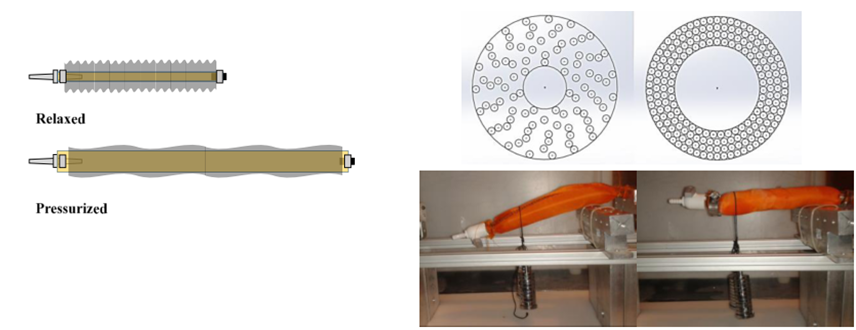
\includegraphics[width=\textwidth]{IPAM.png}
    \caption{a) Illustration IPAM developed in its relaxed and pressurized state, the small radial expansion and large axial expansion is appreciated. b) Cross-sectional view of the jamming effect ongoing inside the actuator (top), and bending effect (bottom) caused by heavy load, left hand side image, and correction of the bending using the jamming effect, right hand side image. \cite{Sridar2016}. }
    \label{fig:IPAM}
\end{figure}

The experiments performed in the paper showed that this innovative soft actuator is 33\% more efficient in comparison to a McKibben muscle using hydraulics. Furthermore, this actuator can be easily manufactured with off-the-shelf components. On the other hand, the convenience of using both pneumatic and hydraulic muscles for performing pulling instead of pushing tasks, is to prevent the bending effect caused when the actuator is fixed in one of its ends and has a heavy load attached to the other end. The latter effect is amplified for pushing tasks being one of the main drawbacks of the proposed actuator concept. However, a proposed solution is to use the principle of jamming by filling the gap between the inner and outer layer with granular media which will jam when the actuator is pressurized (\autoref{fig:IPAM}). Another IPAM development can be found in \cite{Hawkes2016} which implemented a very similar concept as the previously mentioned, however, this IPAM managed to achieve a strain of 300\% the length of the developed actuator whilst the previously mentioned IPAM only achieved a 100\% strain. The improvement in the achievable strain was mainly to the complete restriction of the stretchable material in the inner layer to only expand along its axis and not radially. Furthermore, the main benefits of IPAM in comparison with PAM are reported as follows: high strain and nearly linear control (since no radial deformation is present). The ability to achieve high strains make these soft actuators suitable for joints like the elbow.

\subsubsection{Cable-driven Actuators} \label{sec:cable-driven}

Another actuation technology implemented in soft orthoses are the Bowden cables in combination with electrical motors. Following the same principle as pneumatic muscles, this technology relies on generating tensions along a cable which, with a right positioning along the human lower limb, can transmit torques to the human body. The work in \cite{asbeck2013biologically} presents the design and implementation of a battery operated soft exosuit built with Bowden cables (\autoref{fig:bowden_exo}). 
\begin{figure}[hbtp!]
    \centering
    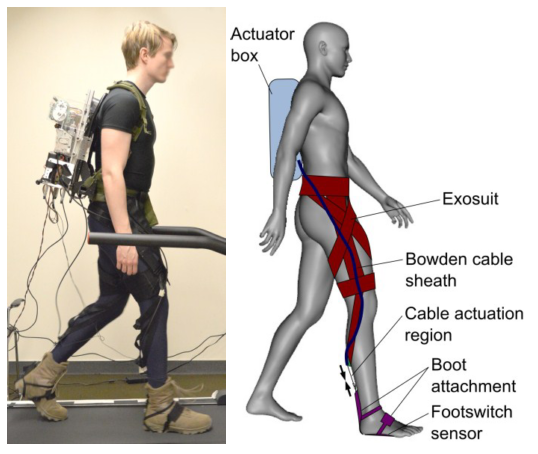
\includegraphics[width=0.5\textwidth]{BowdenExosuit.png}
    \caption{a) Developed Bowden cable-based soft exosuit prototype. b) Illustration of the initial design concept highlighting the main parts of the soft exosuit. \cite{asbeck2013biologically}. }
    \label{fig:bowden_exo}
\end{figure}

The exosuit is based on the leg's muscles functionality during normal walking, with the objective of assisting the forward propulsion stage of the gait. The soft exosuit structure made of fabrics is attached to the waist and above the knee, from the former the Bowden cable follows a path of webbing straps into the lower limb, ending at the ankle. In order to minimize the webbing strap structure chaffing and displacement when tensions are created along it, the strap along the waist of the user terminates at the hip since it is a bony part, i.e. there is almost no muscle and fat tissue between the skin and the bone, ultimately improving the exosuit stiffness. On the other hand, the suit delivers 18\% and 30\% of the torques required for normal walking on the knee and hip, respectively. However, despite the innovative design, the exosuit structure have limitations on the degree of compliance and stiffness, resulting in an approximately 13 cm displacement of the exosuit, when the Bowden cable is actuated. The biggest reported limitation during the experiment was the inefficiency of the Bowden cables, almost 45\% of the mechanical power generated by the actuator is lost, mainly in friction. However, the implemented multi-joint concept allows the actuation of two joints using a single actuator.

Following the multi-joint actuation concept, another soft exosuit is designed in \cite{Bartenbach2015} with the objective of not only providing assistance but also to enable impaired users. The concept (\autoref{fig:bowden_exo2}) exploits the benefits of using a single Bowden cable actuator to control more than one joint, multi-joint actuation. The difference in this case is the deep analysis performed regarding the compatibility of the joints, taking into account synergy of torque and equal polarity of torque, as well. In order to assist the desired movements of sit-to-stand, walking and stairs ascend, the knee and the hip joints were selected as the most suitable combination. Despite the fact the work was limited to describe the concept and design, by analyzing the selected joint combination it is expected to support the movements of sit-to-stand and stairs ascend.
\begin{figure}[hbtp!]
    \centering
    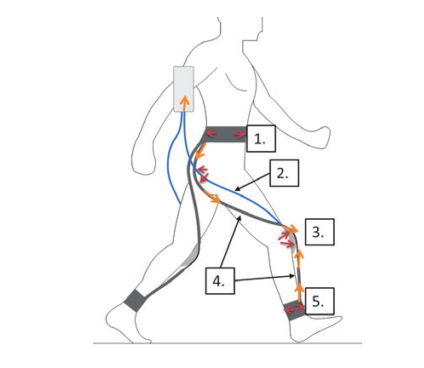
\includegraphics[width=0.7\textwidth]{BowdenExosuit2.png}
    \caption{Soft exosuit implementing the multi-joint actuation concept. A Bowden cable actuates the suit (2) by contracting the webbing element anchored at the hip (1) and shank (5). Reaction forces and actuation forces are represented in red and orange arrows respectively. \cite{Bartenbach2015}. }
    \label{fig:bowden_exo2}
\end{figure}

The next follow up on the concept of multi-joint actuation is documented in \cite{Ding2014} where a testing platform for soft exosuits was developed. The aim of this platform is to study the performance of the multi-joint actuation concept when being implemented in different soft exosuits. The off-board platform integrates the Bowden cable actuators and the sensors required to evaluate their performance. In addition, this platform can deploy sensors to be attached to the exosuit and compare relevant metrics such as mechanical power efficiency. This platform, which can be re-configurable to meet different applications, has been used to evaluate the advantages of implementing single joint and multi-joint actuation \cite{Ding2016}, highlighting the benefits of the latter. Furthermore, the study performed with the aid of this platform provided designing parameters for the development of an exosuit, in other words, the multi-joint platform assists the designing phase, ultimately reducing designing times.

\subsubsection{Shape Memory Materials}

The main two groups of shape memory materials implemented in soft robotics are: shape memory alloys (SMA) and shape memory polymers (SMP). Both technologies function under the same principle: they are able to switch into a different shape when a stimulus such as heat is in contact with them. Nevertheless, there are some differences to be mentioned. The SMA have to main phases, one for high temperature (austenite) and one for low temperature (martensite), when they suffer deformation while being in the martensite phase they can recover from the deformation by exposing them to heat, therefore SMA convert the energy from heat into mechanical energy to return to their original shape \cite{ImagesScientificInstrument2016}. This property is usually exploited to cause contraction changes in the mate-rial (\autoref{fig:SMA}). Therefore, SMA are commonly used in tendon-driven applications.
\begin{figure}[hbtp!]
    \centering
    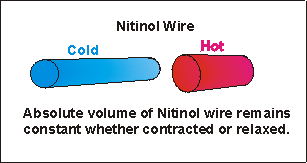
\includegraphics[width=0.5\textwidth]{SMA.png}
    \caption{Shape memory alloys made of Nitinol. The contraction effect under the increase in temperature is illustrated \cite{ImagesScientificInstrument2016} }
    \label{fig:SMA}
\end{figure}

The implementation of SMA into robotic applications have three main challenges to be addressed: response speed, high power consumption and low operational bandwidth. SMA make use of the Joule effect present in metals when an electric current flows through it, which generates heat. Depending on the metals used in the alloy, the amount of heat required for the SMA to recover from deformation is high enough to melt plastics, this excess of energy is what makes SMA inefficient \cite{Bundhoo2009a}. Furthermore, the large time required to cool down the SMA in order to repeat a cycle of deformation-recovery is another limitation which limits the operation frequency. This cooling process is usually performed by air convection which explains the large time (several seconds) required \cite{Bundhoo2009}. Therefore, SMA have been found to be unsuitable for orthoses or prostheses. However, plenty of authors have successfully developed the latter devices, in both rigid \cite{tarkesh2007} and soft variations \cite{Stirling2011}, capable of assisting human motions proving to be suitable for applications such as clinical rehabilitation where slow and repetitive cycles are required \cite{Pittaccio2009,Chenal2014}. Two comprehensive reviews documented in Pittaccio and Viscuso \cite{pittaccio2012shape} and Coral et al. \cite{Coral2012} illustrates the many other applications where SMAs are being implemented in the field of rehabilitation, such as: re-positioning, muscle toning, functional exercise and assistive robotics. Moreover, the review done by W. Coral \cite{Coral2012} also describes many works focused on addressing the SMA limitations.

The very interesting work done by J. Zhang in \cite{Zhang2013a} describes a SMA-based artificial muscle. This configuration facilitates the addition of a cooling system, due to the cylindrical hollow shape of the artificial muscle. Therefore, a mini pump is used to create a flow of air inside the artificial muscle which is able to reduce the cooling time by 10 times. The performance of this artificial muscle is further improved by taking into account the hysteresis behaviour typically found in SMA when shifting between the low and high temperature phases. Furthermore, there is again evidence of trying to replicate the muscle-tendon functionality, in this case by adding a spring in series with the artificial muscle which aids the SMA recovery phase and simulate a more realistic condition to the one at which the human muscles are subjected. The author is the first one able to model this behaviour and develop an adequate controller, which can be implemented in other scenarios involving SMA. Finally, this artificial muscle is implemented into an active foot orthosis (\autoref{fig:SMA_orthosis}) which achieves large contractile forces by using in parallel more than one SMA wire to form each of the pulling tendons. The main drawbacks were having low efficiency and low operational bandwidth.

\begin{figure}[hbtp!]
    \centering
    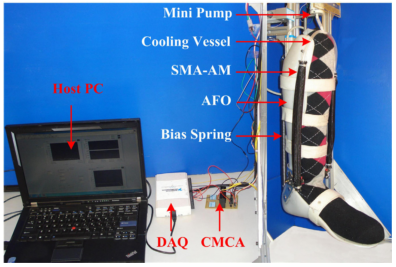
\includegraphics[width=0.7\textwidth]{SMAOrthosis.png}
    \caption{Developed soft orthosis for the ankle joint. The developed SMA artificial muscle along the main parts are highlighted. \cite{Zhang2013a}. }
    \label{fig:SMA_orthosis}
\end{figure}

Many attempts to improve SMA bandwidth have been made and since the theoretical bandwidth for a SMA is 3\% of its length, the most obvious approach is to increment the length of the SMA wire for a particular actuator but without increasing the length of the actual actuators. The latter can be achieved by using pulleys on each end-point of the actuator to develop, which allows the SMA wire to effectively increase its length without increasing the actuator length. However, implementing solely pulleys in a soft actuator greatly reduce compliance, increase the actuator weight and may cause twisting between the individual turns of the SMA wire. Therefore, a new approach described in \cite{Villoslada2015} proposes the implementation of Bowden cables outer sheath to contain the SMA wires inside. This concept allows the SMA to be directed in many ways to the point of interest, allowing the actuator to have different shape that can be compliant with the user's body, e.g. the SMA can be wrapped around the user's arm in a solenoid-like shape which also increases the SMA wire length (\autoref{fig:flexible_actuator}). Furthermore, pulleys are also implemented to allow the SMA to have a maximum number of three turns contained inside the Bowden sheath. Two main drawbacks were discovered during an experimental testing: SMA wires were twisting between each other which caused high friction losses and prevented the SMA to recover its initial length completely; the other drawback was the Bowden sheath material which was found to have low force transmission efficiency. In order to solve the latter, the Bowden cable sheath made of nylon was replaced by flexible tubes of Polytetrafluoroethylene (PTFE) and every SMA wire turn was individually encased in a narrow-gauge sheath. The final experiments showed that the developed actuator is able to contract 9\% of its length which is three times the theoretical contraction length of an SMA wire.

\begin{figure}[hbtp!]
    \centering
    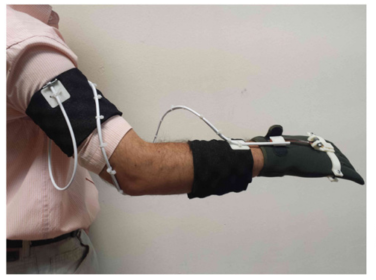
\includegraphics[width=0.5\textwidth]{FlexibleActuator.png}
    \caption{Flexible actuator around the arm in a wrist exoskeleton prototype. \cite{Villoslada2015}. }
    \label{fig:flexible_actuator}
\end{figure}

Shape memory polymers (SMP) are a little bit more complex than SMA. They have two main phases: a glassy state (high stiffness) and a rubbery state (low stiffness). Furthermore, when they are in their rubbery state, they can be deformed by applying small forces and preserve the deformation by cooling the SMP. In this state, the SMP can be considered rigid and it has to be heated to the point of the transition temperature to return to its original shape, hence having shape memory. This property of preserving a deformation is analyzed by K. Takashima et al. \cite{Takashima2010} in an attempt to boost the McKibben artificial muscle performance. McKibben actuators are unable to maintain their contraction shape unless precise and continuous control is implemented which cause premature wear on controlling elements as well as increase energy consumption. Therefore, a SMP is embedded into the McKibben braid which, by controlling the SMP temperature, allows the artificial muscle to hold its contracted position as illustrated in \autoref{fig:mckibben}. It is worth mentioning that SMP can be stimulating in different ways to obtain the change of shape, such as infrared light, electric field, magnetic field and even manipulating the material water content. In this work, the SMP made use of a heating source as well as compressor which drastically limited the developed actuator portability, but as previously mentioned, different stimulus sources can be used for different SMP.

The positive factors when comparing a SMA with a SMP are described, being the SMP benefits: light weight, low cost, rigidity in low temperature and flexibility in high temperature, higher strains, hence length deformation (around 400\% in comparison with 7\% for SMAs) and 3D shapes can be easily created. Furthermore, the main positive aspects of the improved McKibben are: allows rigidity fixing, the parameter to control stiffness can be used to control actuation and controllability of the actuator surface by individually stimulating certain segments of the SMP.

\begin{figure}[hbtp!]
    \centering
    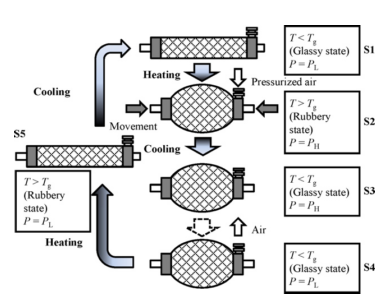
\includegraphics[width=0.8\textwidth]{Mckibben.png}
    \caption{Schematic illustrating McKibben with embedded SMP functionality \cite{Takashima2010}. $T_g$: transition temperature, $P_H$: high pressure, $P_L$: low pressure. }
    \label{fig:mckibben}
\end{figure}

\subsection{Soft Perception Technologies}
\subsubsection{Liquid metal alloys embedded into elastomers}

Strain soft sensors made of liquid metal alloys embedded into soft materials are being implemented into soft orthoses, such as the one in \cite{park2011bio}. The materials used in this case were Eutectic Gallium Indium (eGaIn), as the liquid metal alloy and flexible silicon rubber layer, which creates a really flexible sensor (\autoref{fig:strain_sensor}). The sensor was implemented to measure changes in the ankle joint proportional to the skin strain which it was attached to, by measuring the changes in resistance caused by the variations in the path length and cross-sectional area of the channel containing the liquid metal. Nevertheless, the developed soft orthosis implemented two other non-soft sensors: an inertial measurement unit (IMU) as an angle position detection and a pressure sensor attached to the shoe insole to detect foot strikes, hence the gait cycle. The developed strain sensor delivered good performance and contributed in the development of a feedback controller for this soft orthosis.

\begin{figure}[hbtp!]
    \centering
    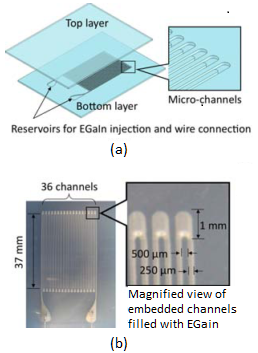
\includegraphics[width=0.6\textwidth]{StrainSensor.png}
    \caption{Soft strain sensor. The microchannel filled with liquid metal can be appreciated in: a) concept design and b) the prototype. \cite{park2011bio}. }
    \label{fig:strain_sensor}
\end{figure}

Liquid metal alloys are also implemented in \cite{Park2012}, as previously described, in the form of embedded muscle-sensor units (\autoref{fig:soft_sleeve_sensor}). The soft strain sensor was able to estimate the contraction length of a pneumatic muscle by measuring its radial expansion. In order to preserve softness, thin flexible copper wires were embedded into the cylindrical soft orthosis to obtain the sensor readings.

\begin{figure}[hbtp!]
    \centering
    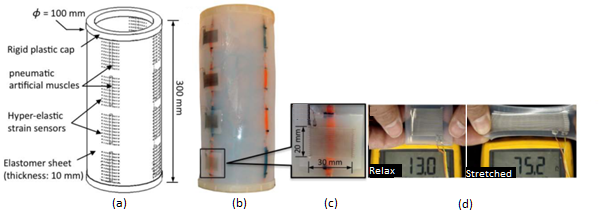
\includegraphics[width=0.9\textwidth]{SoftSleeveSensor.png}
    \caption{a) Design concept. b) Developed prototype. c) Magnified view of the embedded sensor-actuator concept. d) Soft strain sensor change in resistance during stretch. \cite{Park2012}. }
    \label{fig:soft_sleeve_sensor}
\end{figure}

Taking a step further the application of soft strain sensors with eGaIn, in \cite{mengucc2013soft} is presented in a wearable soft suit capable of sensing the joint angles of the hip, knee and ankle joints (\autoref{fig:Sensing_suit}). With the sensors properly positioned along the lower limb, by measuring the strain caused by the joint rotation, the join angle can be known. The sensors were able to track motions with a mean absolute error of 8\textdegree{}, being the most precise tracking achieved on the hip joint and the less precise on the ankle joint. In the mentioned work, only sagital plane motions were measured, however, due to the great success and linearity of the sensors, they are planned to be implemented to measure motions in the frontal plane as well. The complete suit characterization can be found in \cite{mengucc2014wearable}.

\begin{figure}[hbtp!]
    \centering
    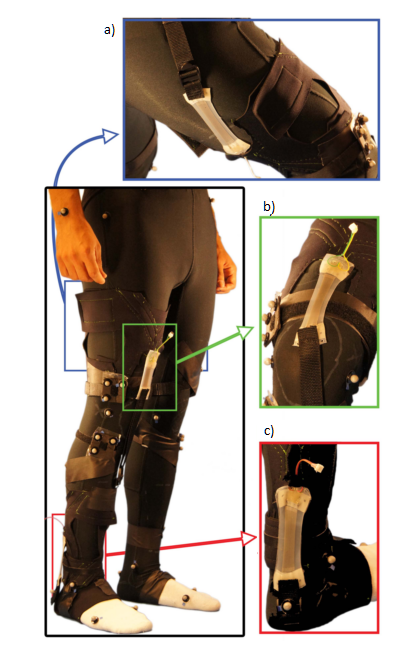
\includegraphics[width=0.4\textwidth]{SensingSuit.png}
    \caption{Implementation of soft strain sensors into a Soft sensing suit, from top to bottom: hip sensor, knee sensor and ankle sensor position. \cite{mengucc2013soft}. }
    \label{fig:Sensing_suit}
\end{figure}

On the other hand, a potentially improved version of these soft strain sensors is presented in \cite{Chossat2013} where the highly stretchable elastomer is filled with two different conductive liquids, a traditional liquid metal and an ionic solution, instead of one. Interconnecting the strain soft sensor with the external application has been a big challenge, since the strain caused by the connection, usually soft wires, affects the sensor accuracy by increasing the total electrical resistance and by generating additional strain. Nevertheless, the ionic solution is intended to decouple the signal routing part from the sensing part in order to solve the latter challenge, creating a noise-free interface with the external application (\autoref{fig:hybrid_strain_sensor}).

\begin{figure}[hbtp!]
    \centering
    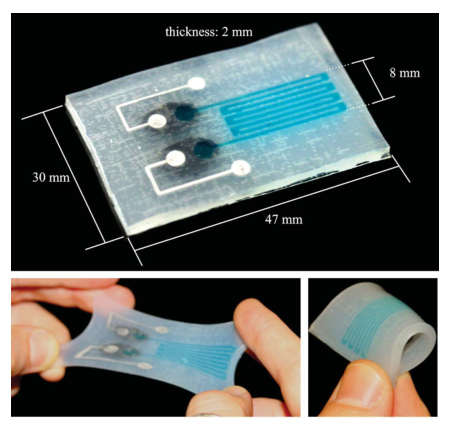
\includegraphics[width=0.5\textwidth]{HybridStrainSensor.png}
    \caption{Hybrid soft strain sensor, the interface between the liquid metal and the ionic solution can be clearly seen in dark areas. \cite{Chossat2013}. }
    \label{fig:hybrid_strain_sensor}
\end{figure}

One direct implementation of the embedded microchannel with conductive fluid sensors, can be seen in a recent improvement to the McKibben type PAM (\autoref{fig:braided_sensor}). McKibben actuators were strongly adopted in soft robotics applications and there is plenty of information in the literature about their implementations, modelling, etc. However, accurately sensing these actuators parameters such as deformation and force when they are pressurized was still a challenge being addressed in many forms such as: cylindrical dielectric elastomers with carbon grease disposed on their surface to function as electrodes \cite{Goulbourne2007}; and attaching to the actuator an elastomer sheath with microchannels filled with conductive fluid which surround the actuator in a helical shape \cite{Park2013}. Both the microchannels and the electrodes represent a resistor which will change its physical dimensions, by extension its electrical resistance, when the actuators compress or stretch which provides a measure of the actuator deformation. Furthermore, the idea of a helical path surrounding the actuator was extended to a solenoid shape and to the so called 16 helices shape, as shown in \cite{Felt2014,Felt2015}. From the electric circuit created, it is possible to measure both the output force and length deformation of the actuator by correlating them with the circuit resistance and inductance respectively. This work proposed the implementation of conductive wires to build the reinforced braid of a McKibben actuator allowing the actuator to `sense', from there the given name of `Smart Braid', creating a solenoid like circuit from which the inductance can be measured using a couple of mathematical approximations such as: the Neumann approximation (for the 16 helices shapes) and the long solenoid approximation, being the former one the most accurate and general; but at the same time the most expensive in terms of computation. The author exerts that this new sensing concept can be applied to multitude of scenarios in soft robotics, which includes soft orthosis.

\begin{figure}[hbtp!]
    \centering
    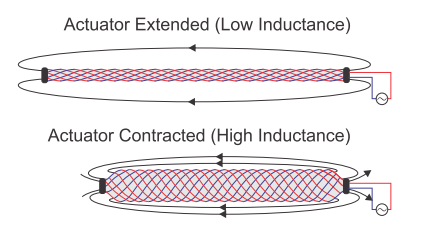
\includegraphics[width=0.5\textwidth]{BraidedSensor.png}
    \caption{`Smart Braid' concept. The variation in the actuator length cause a change in the electric circuit inductance. \cite{Felt2015}. }
    \label{fig:braided_sensor}
\end{figure}

\subsection{Control Technologies} \label{sec:controlSystems}

One of the successfully implemented control systems is documented in \cite{park2011bio}, which is the ankle soft orthosis previously mentioned. The control system is comprised of several micro-controllers for parallel processing, and is divided into four main stages: sensing, signal processing, control and actuation (\autoref{fig:control_system}). The soft orthosis makes use of three different sensor technologies which requires different sampling and signal processing algorithms for each one, the IMU being the most complex one. Thereafter, another micro-controller with access to all the sensors, makes the decision to activate the solenoid valves that control the pneumatic muscles by generating a pulse width modulating (PWM) signals which in combination with binary on/off valves are able to perform a proportional control type. No mathematical model was deducted to describe the non-linear behaviour of the pneumatic muscles, instead, simpler controller approaches as feed forward and feedback controller were being implemented, with the latter being able to achieve a response time of 500 ms when a perturbation was present on the system, such as letting a weight hang from the device toe. The feedback controller made use of a soft strain sensor (previously mentioned) to correct the ankle angle. Finally, although the controller performance is good it is still not enough to provide active gait assistance nor to predict user intentions. Another drawback, minor in this case, is that the system requires calibration every time a new user wears it. Nevertheless, the developed soft orthosis is suitable for rehabilitation because it can achieve a dorsiflexion of 12\textdegree{} and 20\textdegree{} when foot was at resting position, and when foot was forced to a plantarflexion position, respectively; in addition, the perception system could provide the clinician with meaningful data about the patient progress. The previous work was continued in \cite{park2014design} where a new controller was designed by considering the interaction between the soft exosuit and the human body as a black box, i.e. instead of trying to model the non-linear behaviour of the whole system some experiments were performed to obtain a system input/output relationship and after that implement classic control techniques to model a linear time invariant controller. The results were promising since the original complex system was able to perform accurately using simple techniques. Finally, the addition of electromyography sensors was discussed to add the involuntary muscle contractions of the user into the system as a disturbance and improve the accuracy during different scenarios.

\begin{figure}[hbtp!]
    \centering
    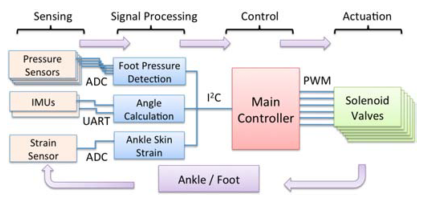
\includegraphics[width=0.7\textwidth]{ControlSystem.png}
    \caption{Control system architecture implemented for the ankle soft orthosis. \cite{park2011bio}. }
    \label{fig:control_system}
\end{figure}

In some cases, the design and development complexity of a controller for soft devices restrain the research extend to focus only on the implementation and study of soft actuation and perception systems. This is the case in \cite{Park2012}, the cylindrical soft sleeve with embedded muscle-sensor units; where the developed controller is well designed but with no close-loop architecture nor complex mathematical model to predict the soft material behaviour. Again, the controller system is integrated by several micro-controller units, each of those communicated with their surrounding neighbours, in fact, each of the 16 nodes embedded into the cylindrical soft sleeve has one. Furthermore, each controller architecture has two layers, one dedicated to the collection of sensor data, intercommunication between the micro-controller units, specify actuation parameters and schedule of tasks. The scheduler is implemented as a means to synchronize the otherwise independent micro-controller units and behave as a network, converting the system into a sequential one instead of a parallel one as previously mentioned. Every unit has four tasks to execute at a given time and a given order: sensing, communicate, process data and actuate. On the other hand, the actuation parameters are generated using a mathematical approximation of the soft material behaviour which assumes no deformation is caused by the compression of the pneumatic actuators, other than the length change present where the actuators are embedded, this means the diameter of the cylinder remains constant as well as the length in the other side of the cylinder. The experiment proved the requirement of a better approximation, since for a desired bending angle of 15\textdegree{}, an actual bending of 11.5\textdegree{} was achieved, and feeding the soft sensors data into the mathematical approximation, a bending of 13\textdegree{} was estimated; therefore, achieving an accuracy of 76\%.

The fact that few soft exosuit developments fully implement a controller system does not imply that no research is being performed in the field. The implementation of current soft actuators into functional devices, as well as the proof of concept of emerging soft actuators are usually followed by an extensive study about modelling their behaviour to translate that information into a controller system. Solely for PMAs several work has been done, even implementing fuzzy logic to achieve better results, in \cite{Chang2015,Skorina2015,Bishop-Moser2015,Hosovsky2016}. The next step in the research cycle of all the soft actuation technologies is to implement the tested models into functional devices, which then will allow new concepts to be developed, hence new modelling research to be performed.

\section{Gaps in the Body of Knowledge} \label{sec:gaps}

The available literature suggests a growing interest in the research and development of soft actuation technologies, soft perception systems, and control systems to pair with the latter two. Also, and following the bioinspiration driving the field of Soft Robotics, many works are attempting to imitate the capabilities of the human musculoskeletal system by developing soft actuator that behave like the human muscle-tendon component. This is more evident when looking at the available works on Pneumatic Artificial Muscles (PAMs) described in \autoref{sec:PMAs}, where an actuator is used as the contractile force generator element (muscle), and a flexible interface (tendon) is used to transmit that force to the desired location. Similarly, established technologies such as electric motors, which are able to deliver forces in both directions of rotation, are being used in combination with Bowden cable to create pulling forces, as mentioned in \autoref{sec:cable-driven}. This type of setup is known as a redundant system because more than one actuator is required to control both directions of rotation of a joint. Moreover, the research and development of new soft materials, such as the SMA and SMP, is also focused on creating materials able to contract when stimulated. There is still plenty of work to be done in this matter, which is why this is identified as one gap in the body of knowledge.

The vast majority of available literature is focused on testing a new soft actuation concept in an open-loop approach, i.e. with no control system implemented. This is caused by the fact that modelling the mechanical behaviour of a soft material is very complex. Even the control system of the most documented work in the literature, the ankle-foot orthosis, does not implement a modelling technique to monitor the behaviour of the PMAs, instead it is focused on extracting as many information as possible from the environment and use this to decide when and how to activate the PMA \cite{park2011bio}. The scarce literature about the control systems of soft robotic applications, as evidenced in \autoref{sec:controlSystems} is identified as another gap in the body of knowledge.

Therefore, two main gaps are considered in the body of knowledge which are addressed by this research. On the one hand, there is still many work to do in understanding the functionality of the human musculoskeletal system, and in developing a soft actuation technology which mimics the functionality of the muscle-tendon component. On the other hand, there is a lack of reliable modelling tools to predict the complex mechanical behaviour of soft materials being used in soft actuation technologies. 

\section{Summary}

According to the literature, the most commonly implemented soft actuation technologies in soft robotic applications for human assistance are: Pneumatic/hydraulic artificial muscles, cable-driven actuators based on electric motors, and shape memory alloys/polymers.  In cable-driven actuators, the amount of generated assistance is proportional to the electric motor mechanical output power. This means, large forces can be generated to even enhance the user capabilities, yet again, the transmission of this forces via the human body prevents this enhancement. A common problem is the relative displacement of the soft structure worn by the user when tensile forces are generated by the pulling action of Bowden cables. Nevertheless, one advantage of this technology in soft exosuits is the `remote' actuation capability, which means that the electrical motors can be placed distal to the joint to be assisted, concentrating the weight of the heavy parts of the soft exosuit in convenient locations of the human body, e.g. as a backpack. Another advantage of this technology is the flexibility of the Bowden cables which allows them to be deployed in many different trajectories along the human body, facilitating the use of the body parts capable of sustaining high forces.

In contrast, the other two soft technologies are commonly placed proximal to the joint to be assisted, which might allow a better distribution of the soft orthosis weight. Recent works have tackled the main limitations of PAMs, SMA and SMP. Particularly, big improvements have been achieved for PAMs and SMA. For the case of PAMs, the traditional and extensively implemented McKibben type muscle have been improved in terms of performance by the development of the Inverse PAM (IPAM). This latter technology surpasses the McKibben type muscle in assistance capabilities, efficiency and controllability. Furthermore, the concept of the IPAM can also be implemented using hydraulics which again comes with several advantages, a crucial one, the amount of exerted force. The main disadvantage of both pneumatic and hydraulic actuators is the need for a compressor unit, which greatly decreases the soft orthosis autonomy and portability. Nevertheless, the recently developed `Hydro Muscle', which uses pressurized water from a home tap, greatly increases the appealing of this technology. In a similar way, the greater efficiency of IPAMs allows portable tanks with pressurized air to be used.

The situation is quite similar for SMAs, many of the limitations from this technology, such as low strain, slow speed response and complex controllability have been addressed and improved. However, this technology is still in its early stages and their main drawbacks, such as high energy consumption and being unsafe for human interactions applications due to the high levels of heat they reach, make them unsuitable to be deployed in real soft robotic applications.

In the field of soft sensors, one of the main advantages of the soft strain sensors is that they can be custom-built to fit any application. When characterizing these sensors, two parameters are always mentioned: the electrical resistance and the gauge factor, the latter relates the strain with the change in resistance. Despite their original purpose of measuring strain changes, they can be used for angle measurements. On the controller side, the amount of research being performed in modelling the complex behaviour of soft actuators is slowly but constantly increasing. Nevertheless, the complexity and time consuming of tackling the latter is evidenced in the scarce literature available.

In summary, this literature review highlighted a very specific and bioinspired trend in soft robotic applications for human assistance, which is mimicking the human musculoskeletal system, specifically the muscle-tendon component. This approach is very compatible with soft technologies that are commonly placed proximal to the assisted joint (PAMs, SMAs, IPAMs, etc.), and many soft artificial muscles have already been developed. These works, however, have mainly focused on the contractile element of the muscle-tendon component, leaving plenty of room to research about the viscoelastic element, the tendon. The most straightforward to study the potential benefits of mimicking the human tendon behaviour, is to incorporate soft materials, to current soft actuation technologies, as part of the mechanism to transmit the generated forces. Essentially, creating a soft artificial tendon. Nevertheless, the success of maturing the previous concept into a soft robotic application greatly depends on having a reliable modelling tool which predicts the mechanical behaviour of soft materials. Finally, as mentioned in \autoref{sec:gaps}, this research aims to address two main gaps in the body of knowledge. On the one hand, the lack of literature about the implementation of soft materials as part of the force transmitting mechanism, which could allow for a better mimicking of the human musculoskeletal system. On the other hand, the lack of a modelling tool able to predict the mechanical behaviour of soft materials.

\newpage\null\thispagestyle{plain}\newpage
\chapter{Mimicking of Human Skeletal Muscle System} \label{sec:mimicHSMS}

\section{Introduction}

Previously, the bioinspired trend of mimicking the human skeletal muscle system, specifically the muscle-tendon component, in soft robotic applications for human assistance was identified. The available literature is mainly focused on the muscle component. In line with the aims of this research, this chapter is focused on understanding the biomechanics of the human body, specifically of the lower limb due to its great contribution on the Activities of Daily Living (ADLs). Therefore this chapter is divided as follows.
Section one focuses on understanding the terminology involved in the biomechanics of the human lower limb. In section two, many clinical trials, also known as gait analysis, are reviewed to characterize the parameters of torque, angle, and power of the human lower limb during ADLs. Section three describes the muscle-tendon component from a mechanical perspective. Section four introduces many recent works and approaches which attempt to translate the functionality of the muscle-tendon component into soft robotic applications. Section five describes how recent works are addressing the lack of modelling tools for soft materials, considering two main modelling approaches: model-driven and data-driven. Finally, the last section presents a summary of the relevant findings of this chapter.

\section{Biomechanics of the Human Lower Limb}

The common terminology used in clinical trials for the lower limb make use of the three planes of action of the human body to name the motion of a given joint of the body. These three planes are called sagital, frontal and transverse (horizontal) \cite{PhysicalSolutions2016}. In combination with these planes there are three axes used to identify specific motions: frontal horizontal axis, vertical axis and sagittal horizontal axis. The positioning of each of them is illustrated in \Cref{fig:body_planes_axes}. The sagital plane divides the body vertically into left and right parts, the frontal plane divides the body vertically into front (posterior) and back (anterior) parts and the transverse plane divides the body horizontally into upper (superior) and lower (inferior) parts.

\begin{figure}[htbp!]
    \centering
    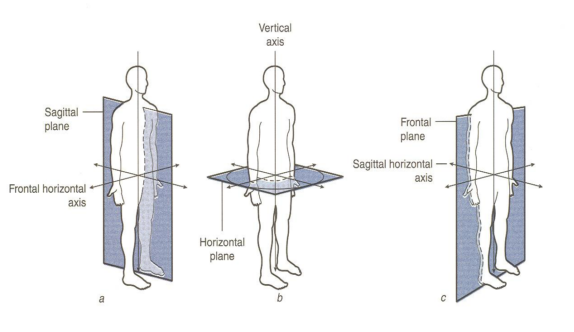
\includegraphics[width=\textwidth]{BoydPlanesAxes.png}
    \caption{Dimensional spaces used to understand human motions: a) Sagittal plane, b)Horizontal plane and c)Frontal plane. \cite{PhysicalSolutions2016}. }
    \label{fig:body_planes_axes}
\end{figure}

Similarly, the motions of the human joints are named according to the plane and axis in which they are executed, which allows for easy recognition of the human body motions (\Cref{fig:lower_motion}). There are ten different motions, grouped into five pairs, governing the lower limb of the body:
\begin{itemize}
    \item Flexion and extension describe the bending motion which decreases, or increases the angle between two parts of the body, respectively.
    \item Abduction and adduction describe the motion away from, or towards the body midline, respectively.
    \item Eversion and inversion of the foot describe the motion away from, or towards the body midline, respectively.
    \item External rotation and internal rotation describe the motion away from, or towards the body midline, respectively.
    \item Horizontal abduction and adduction describe the motion away from, or towards the body midline, respectively.
\end{itemize}

\begin{figure}[htbp!]
    \centering
    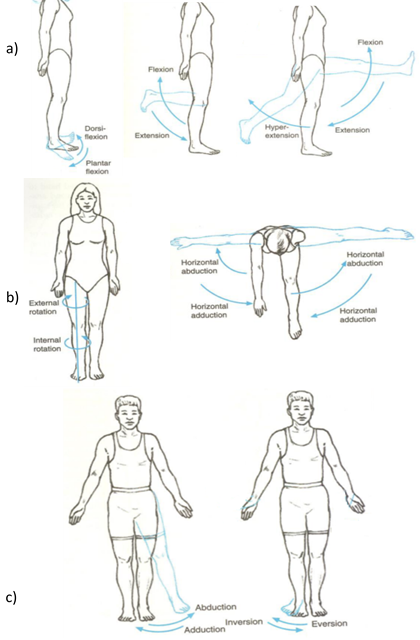
\includegraphics[width=0.8\textwidth]{LowerLimbMotionTerminology.png}
    \caption{Lower limb motions for a) sagital plane, b) horizontal plane and c) frontal plane. Image adapted from  \cite{PhysicalSolutions2016}. }
    \label{fig:lower_motion}
\end{figure}

Having defined all the available movements of the human lower limb, its kinematic and kinetic parameters during activities of daily living are described in the following section.

\section{Characterization of Kinematic and Kinetic Parameters for Activities of Daily Living}
\label{sec:characterizationKKP}

The design process of a wearable robotic device includes the characterization of the kinematic and kinetic parameters (KKP) of the human joints intended to be assisted, which allows the device to be tailored to a particular application, whether assisting an elder adult or allowing a disabled patient to walk. The effectiveness of each prototype is commonly assessed by measuring the metabolic cost reduction delivered to the user while performing an activity \cite{panizzolo2016biologically}. However, the latter requires specialized equipment. An alternative way is comparing the range of motion and torque delivered to the assisted joint with the values commonly found in humans during a certain activity. This type of data is available in gait analysis studies. The data from gait analyses can be used in the development of wearable robotic devices since it can provide design guidelines specific to the activity of interest, and can also be used to assess the degree of assistance provided by a prototype.

The KKP are usually found in clinical studies known as gait analyses. The kinematic parameters describe the human body motion in terms of the joint angle, velocity, and acceleration. The kinetic
parameters describe the forces causing this motion, e.g. joint torque and power. Motion capture is the most commonly used method to extract these parameters. However, other technologies such as soft strain sensors \cite{mengucc2014wearable}, electrogoniometers \cite{wu2011electromyography}, and inertial measurement units (IMU) have also been used. Lastly, it is important to mention that these studies differ between one another in many aspects, in addition to the technology of choice, such as subjects' gender, age, weight, etc., as well as the setup of the experiments.

This section is focused on describing the characterization process which, as previously mentioned, can be used as guidelines in the design of wearable robotic devices. The selected gait analyses in here cover the main activities of daily living (ADLs), which are: walking, ascending/descending stairs, ascending/descending ramps and chair sitting down/standing up. Similarly, the data for the hip, knee and ankle joints is of interest. Finally, relevant information about the gait analyses and the characterization process is described in the following sections.

\subsection{Gait Analysis Data}

Gait Analysis studies provide the description of the performed experiment, including: the number of subjects in the group, subjects' characteristics such as age, weight, height, gender and health condition; experiment characteristics such as walking speed, ramp inclination, stairs geometry, initial sitting position and special conditions, such as, whether subjects are carrying a load or not. The subjects' characteristics are always presented in mean (average) values of the whole group. In a similar way, the derived data (torque and power) is presented in mean values and is normalized using the subjects' height, in the case of the gait cycle speed; and the subjects' weight, in the case of the torque of each joint. The normalization is appreciated in the units for torque and power, being Nm/kg and W/kg respectively. The data used in the normalization process is usually provided as mean values of the subjects' group's height and weight. However, in some studies like the one in \cite{lee2008biomechanics}, the gait cycle speed is not explicitly provided nor it can be calculated because the normalization process is done considering each subject's characteristics and not the mean values of the subjects group. 

From one study to another, the subjects group is expected to be different and diverse among several characteristics. This diversity causes segmentation of the whole group, e.g. in the study performed in \cite{bovi2011multiple}, there is a segmentation of the group in two different ranges of age. One group included subjects from 22 to 72 years old, meanwhile, the subjects from the other group have ages ranged from 6 to 17 years old. The latter presented evidence of age-related differences which disproved the conclusions on previous works where these differences are non-existent. Nevertheless, when no significant difference is appreciated in the data despite the subjects' age diversity, the data is compiled into a single cluster and no segmentation is performed, such as the case in \cite{lee2008biomechanics}.

Motion capture technology allows the extraction of the kinematic parameters, such as the joint angle. Similarly, the kinetics of the human body are obtained using force plates which measure the ground reaction forces, a required parameter to calculate the joint torque and power. Therefore, the set of parameters usually found in gait analysis studies contains the joint angle, joint torque, and joint power. The activity gait cycle is usually presented in a chart accompanied with tables highlighting the maximum, minimum and mean values of the gait cycle. 

For the characterization of the human KKP, the differences between the maximum and minimum values of each parameter, i.e. its range, is of interest. Commonly, these values are provided in the studies in the form of tables and charts \cite{han2011biomechanical,yali2010biomechanics}. It could also be the case where the whole experiment dataset is provided \cite{moore2015elaborate}. When a data table is available, the extraction of the values is straight forward. Nevertheless, cases such as \cite{protopapadaki2007hip,riener2002stair,mcintosh2006gait,roebroeck1994biomechanics,mak2003joint} do not provide any table and the data have to be extracted visually, adding some error to the process and decreasing the data reliability. Likewise, it can be the case for some studies to focus on specific features of the gait cycle, such as maximum and minimum values of each parameter; or not provide one or more of the parameters of interest (angle, torque or power).

\subsection{Extracting Design Guidelines}

Add introductory paragraph to this section.

The variations of the data from one experiment to another can be reduced by focusing on the range obtained from the difference between the maximum and minimum values of each parameter. This is illustrated in \Cref{fig:HipKKPWalking}, despite the variations between the maximum and minimum values from one experiment to another, the actual range of each parameter is similar among all the experiments. The mean range of motion for the hip joint angle throughout different walking over-ground experiments was found to be 44.63\degree{} (\Cref{fig:HipKKPWalking}). Also, the greatest variation between the mean range value and the range value of each experiment is 18\% of the mean value. The previous calculation can be used to decide design parameters of wearable robotic devices, such as which range of motion should be covered by the device depending on which sector of the population is intended to be assisted. Alternatively, the device can be tailored to cover as much of the population as possible by choosing the maximum and minimum values of the range of motion, out of all the experiments. 
\begin{figure}[htbp]
    \centering
    \begin{subfigure}[b]{0.75\textwidth}
        \centering
        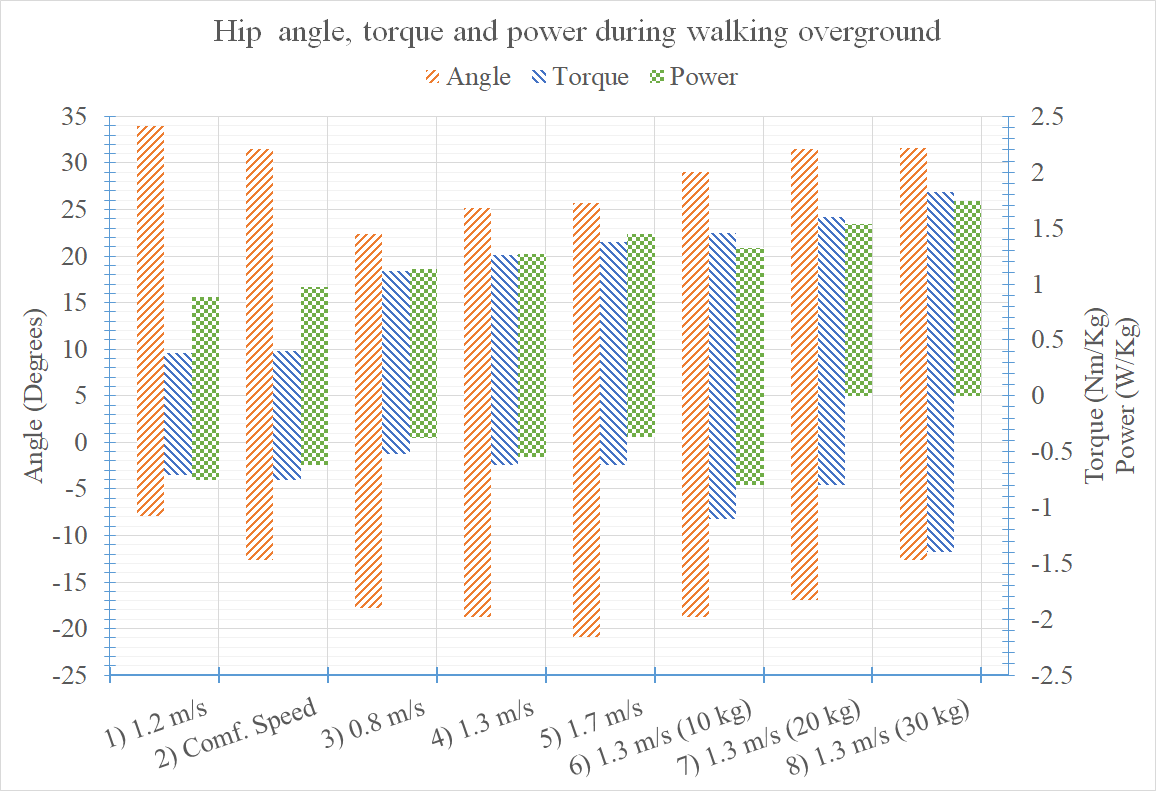
\includegraphics[width=\textwidth]{HipKKPWalkingExcel.png}
        \caption{Hip joint characteristics for walking over ground activities. The weight next to the name of some activities dictates the load carried by the subjects during the experiment \cite{solis2017characterization}. Data collected from: (1) \cite{bovi2011multiple}, (2) \cite{lee2008biomechanics}, (3-8) \cite{han2011biomechanical}. }
        \label{fig:HipKKPWalking}
    \end{subfigure}
    \hfill
    \begin{subfigure}[b]{0.75\textwidth}
        \centering
        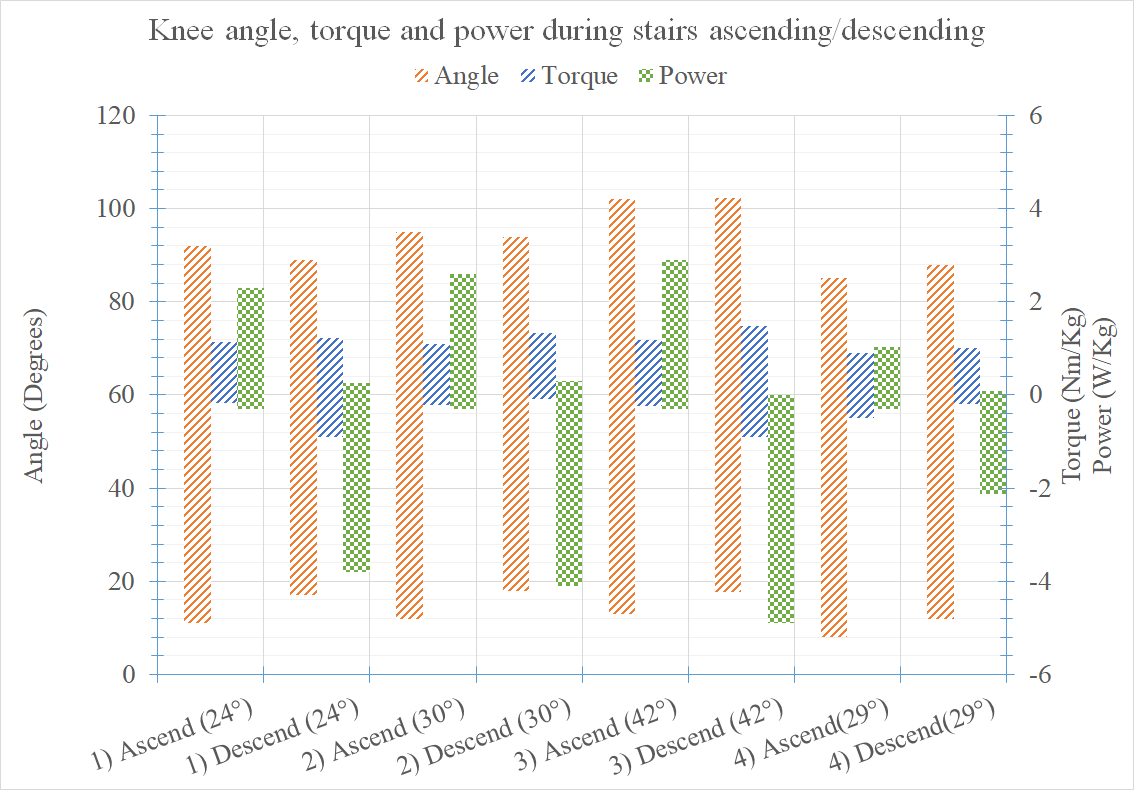
\includegraphics[width=\textwidth]{KneeKKPStairsExcel.png}
        \caption{Knee joint characteristics for several stairs ascending/descending experiments. The number enclosed in brackets represents the stairs slope. Data collected from: (1) \cite{riener2002stair}, (2-4) \cite{reid2007knee}. }
        \label{fig:KneeKKPWalking}
    \end{subfigure}
    \caption{Clustered-stacked bar charts of reviewed gait analyses \cite{solis2017characterization}. }
    \label{fig:clusteredMain}
\end{figure}

Different design guidelines can be extracted when visually analyzing other parameters together. For example, in \Cref{fig:KneeKKPWalking} , the parameters of the knee joint are now compared against many experiments of stairs ascending/descending. Now, the main feature is not the range of motion of the knee, but the characteristics of the torque values. They appeared mirrored, in other words, the torque values required for descending stairs are of similar magnitudes but opposite in direction. Also, the amount required for ascending stairs is generally twice as much as the amount required for descending stairs. The latter illustrates an optimization opportunity. When designing a wearable robotic device for human assistance, the actuator is chosen to satisfy a certain torque range of a particular activity. Without the characterization of the parameters performed, the actuator is most likely to be oversized to comply with the most demanding part of the activity. However, a different approach could be proposed: agonist-antagonist actuators; a technique implemented in several wearable robotic devices which at the same time complies with the actual functionality of the human skeletal muscle system.

Another useful way of extracting design guidelines from the gait analyses is to plot the range of a specific parameter against different ADLs. To the best of the author's knowledge, this approach has only been documented once in \cite{rowe2000knee}, where the range of motion of the knee joint is compiled into a chart for 11 different ADLs. This concept, illustrated in \Cref{fig:HipTorqueRange}, can provide insight of two important design parameters. On the one hand, the actuators meant for this application must be able to deliver torques in both directions of rotation, i.e. clockwise and anti-clockwise. On the other hand, the selected actuation technology must meet the torque requirements of the activity of interest, illustrated in \Cref{fig:HipTorqueRange}. \Cref{fig:HipTorqueRange} was constructed using the mean range of the hip joint torque during different activities \cite{bovi2011multiple,lee2008biomechanics,han2011biomechanical,protopapadaki2007hip,riener2002stair,mcintosh2006gait,roebroeck1994biomechanics,mak2003joint}.

\begin{figure}[htbp!]
    \centering
    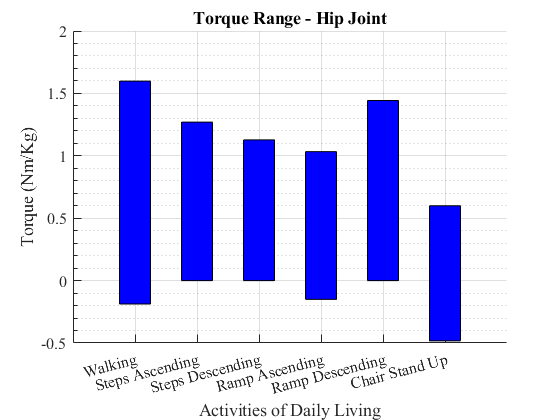
\includegraphics[width=0.8\textwidth]{HipTorqueRange.png}
    \caption{Torque range values during several activities. The values for the maximum and minimum torque are mean values from the data of all the different gait analysis experiments enclosed in one main activity. \cite{bovi2011multiple,lee2008biomechanics,han2011biomechanical,protopapadaki2007hip,riener2002stair,mcintosh2006gait,roebroeck1994biomechanics,mak2003joint,solis2017characterization} }
    \label{fig:HipTorqueRange}
\end{figure}

Another alternative of visual representation of the data can be done by grouping the range of a specific parameter and comparing it with any of the subjects' physical characteristics, e.g. the age range. This is illustrated in \Cref{fig:KneeRangeAge}, where the dependency of the subjects' age with the knee range of motion is evidenced. The colour code used in \Cref{fig:KneeRangeAge}, the age ranges and knee ranges of motion are presented in \Cref{tbl:KneeRangeMotionage}. The chart shown in \Cref{fig:KneeRangeAge} concentrates the data from three different gait analyses, in which six age groups are contained. The approach used in \Cref{fig:KneeRangeAge} is to overlap areas of different colours, each area represents the range of motion of the knee for a specific age range. The area in which several areas intersect can be appreciated due to the enabled transparency property. Nevertheless, the areas where three and two areas are intersected are manually highlighted by a surrounding solid line and dotted line respectively, to improve their visualization. This simple intersection of areas can provide information regarding the required range of motion to be delivered by the wearable robotic device, depending the sector of the population focused on.
For example, if a wearable robotic device was aiming to assist the population sector aged from 50 to 70 years old, then a range of motion of the knee joint from 5{\textdegree} to 63{\textdegree} would be enough to cover the mentioned population. The range of motion is taken from the triple intersection of areas illustrated in \Cref{fig:KneeRangeAge}, which can provide a certain degree of confidence since three different clinical studies were compared. This approach can be used to compare other characteristics, e.g. subject's weight against torque. Summarizing, the areas overlapping approach can provide guidelines to avoid oversizing of the wearable robotic device to be developed by analysing the intersection of different areas which ultimately provides a degree of confidence when deciding design parameters.

\begin{table}[htb!]
\caption{Colour code used in \Cref{fig:KneeRangeAge} for each combination of age range and knee range of motion  \cite{solis2017characterization}.}
\label{tbl:KneeRangeMotionage}
\begin{tabular}{c|c|c|c}
\hline
Colour Code & Knee Range of Motion (\degree{}) & Age Range (Years) & Clinical Study \\
\hline
Red         & 2.2 - 67.4               & 49 - 90           & \cite{rowe2000knee}       \\
Green       & 5 - 66.5                 & 6 - 17            & \cite{bovi2011multiple}        \\
Blue        & 4.5 - 63.5               & 22 - 72           & \cite{bovi2011multiple}           \\
Yellow      & 0 - 69                   & 18 - 30           & \cite{lee2008biomechanics}        \\
Magenta     & 0 - 69                   & 50 - 70           & \cite{lee2008biomechanics}     \\
Cyan        & 8 - 63.6                 & 23 - 27           & \cite{han2011biomechanical}    \\  
\hline
\end{tabular}
\end{table}

\begin{figure}[htb!]
    \centering
    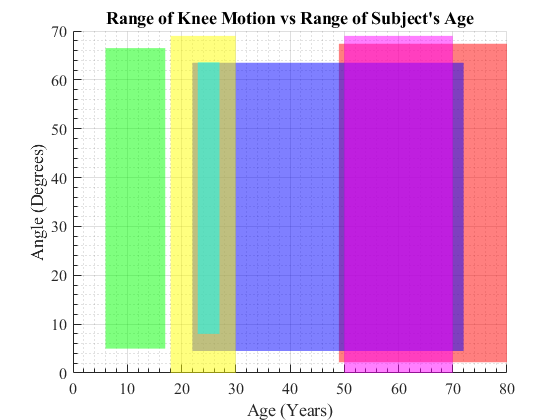
\includegraphics[width=0.7\textwidth]{KneeRangeMotionAge.png}
    \caption{Comparison between subjects' age and the knee range of motion during walking over ground. The areas surrounded by solid lines and dotted lines represent the intersection between three and two areas, respectively. The overlapping squares highlight the great similarity among the range of motion despite subjects' age. The data used to create this chart is presented in \Cref{tbl:KneeRangeMotionage} \cite{solis2017characterization}. }
    \label{fig:KneeRangeAge}
\end{figure}

In this section the process of characterizing the human lower limb kinematics and kinetics parameters during some ADLs was described. The relevant information provided in gait analysis experiments, and the challenges faced when extracting it from the clinical trials, were described. Data compiled for the activities of walking, ascending/descending stairs, ascending/descending ramps and chair standing up were presented in the form of clustered stacked bar charts. This type of chart allowed quick and easy detection of similarities between several clinical trials of the same activity. In contrast, the spotted differences, as the ones for the knee torque values during ascending/descending stairs, are indicators for optimization opportunities where instead of using a single actuator to satisfy the torque range, an agonist-antagonist system could be more suitable.

The reliability of the data can also be observed using the type chart of overlapping areas with subjects' ranges of age against the knee ranges of motion. In other words, the specific ranges in which the data from different experiments overlaps, gives a measure of consistency which can be used to tailor the developed wearable device coverage. 

The chart style with ranges of motion versus activities, facilitates the choice of the actuator type and dimension (depending on the activities of interest). The styles used to represent the charts were kept as simple as possible while providing useful information about the KKP. However, more complex plotting methods can be used. Finally, a total of 12 charts were produced in Excel\textregistered{} using the compiled data from the gait analyses. In favour of keeping the length of this section adequate, only two out of the 12 charts were included in here. The remainder charts were moved to \Cref{appendixA}.

\section{The Muscle-tendon Component} \label{sec:muscle_tendon}

Having defined the terminology involved in the biomechanics of the human skeletal muscle system, and characterized the kinetic and kinematic parameters of its lower limb, this section focuses on describing the muscle-tendon component from a mechanical point of view. 

In the literature, the mechanical model commonly used to describe the mechanical behaviour of the muscle-tendon component is the Hill's model \cite{hill1938heat}. This model is considered to be the most representative of all the available models \cite{zhang2012sma}. Hill's model describes the skeletal muscle as a three elements system, which contains a contractile element, a passive element, and a series element. The contractile element (CE) represents the muscle fibres in charge of generating the contractile forces, the parallel (passive) element (PE) is formed by the tissue surrounding the muscle which prevents it from overstretching, and the series element (SE) represents the human tendon, as illustrated in \Cref{fig:hillModel}.

\begin{figure}[htb!]
    \centering
    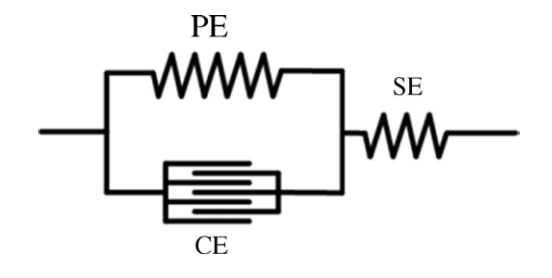
\includegraphics[width=0.4\textwidth]{HillModel.png}
    \caption{Hill's model of the skeletal muscle. The contractile element (CE), the parallel element (PE) and the series element (SE) are shown \cite{hill1938heat} }
    \label{fig:hillModel}
\end{figure}

Hill's model makes the important assumption of considering the SE to be purely elastic, i.e. the deformation of the element is entirely dependent on the force applied to it. Nevertheless, the non-linear viscoelastic properties of the human tendon are acknowledged in his work. The latter simplification is a common practice among studies of the skeletal muscle system because the muscle and tendon are studied as a whole (muscle-tendon component) \cite{zajac1989muscle}. Evidence of the actual benefits of this simplification is found in the literature for the field of robotics exoskeletons. The complex muscle-tendon model developed in \cite{lloyd2003emg}, considered the viscoelastic properties of the human tendon to estimate forces and joint torques in real time. The model achieved high accuracy at the cost of high computational load. In an attempt to reduce the computational load, the assumption of an infinitely stiff tendon was made which proved to be reliable as well \cite{sartori2009stiff}.

In a similar way, developments in the field of soft robotics which are inspired in the skeletal muscle system functionality are also based in Hill's model, as highlighted in \Cref{sec:SoftActuation}. Commonly, springs \cite{park2011bio} or Bowden cables \cite{Zhang2013a} are implemented as the SE of the muscle-tendon model. Nevertheless, the fact is that the human tendon has viscoelastic properties \cite{maurel1998biomechanical}. At the time of starting this research, the documented works in the literature were mainly focused on developing and testing soft materials to be used as the contractile element in soft artificial muscles. The latter, previously identified as a research opportunity, indicates that the viscoelastic properties of soft materials have not been studied with the aim of developing a soft artificial tendon, which in combination with current soft artificial muscles could deliver better performance in soft robotic applications for human assistance.

The first step towards the investigation on the potential benefits of adding viscoelasticity, in the form of a soft SE, to soft actuators is described as follows. As a starting point, the mechanical properties of the human tendon must be investigated. Due to the large contribution of the knee joint in the ADLs, the present investigation is focused in this joint of the human lower limb. Subsequently, the selection and characterization of many soft materials with mechanical properties similar to the human tendon, is proposed. The extracted properties from the studied soft materials and from the human tendon are compared against each other. This comparison analysis has the potential of providing evidence on the benefits and disadvantages of implementing a viscoelastic element as the way to transmit tensile forces in soft orthoses and soft exosuits.

\subsection{Viscoelasticity of the Human Tendon} \label{sec:viscoelasticity}

Tendons are connective tissues that link muscles with bones. As previously mentioned, the human tendon has a non-linear viscoelastic behaviour. This means that the deformation experienced by the material when a force is applied to it, is not proportional to the force through the whole range of possible deformations, and also that it is dependent on the history of previous deformations. At rest, the collagen fibres (core components of tendons) are in a relaxed wavy state. When the tendon experiences a tensile force, the collagen fibres are easily stretched and realigned, opposing little resistance to deformation. However, when the collagen fibres are completely stretched they begin to offer more resistance to deformation which is proportional to the applied force. Finally, fibres can be stretched to their limit and failure of the tendon will occur \cite{nordin2001basic}. This non-linear response to the applied deformation is better explained using \Cref{fig:tendonSS} where the characteristic S-shape curve for tendon stress-strain graph is appreciated.

\begin{figure}[htb!]
    \centering
    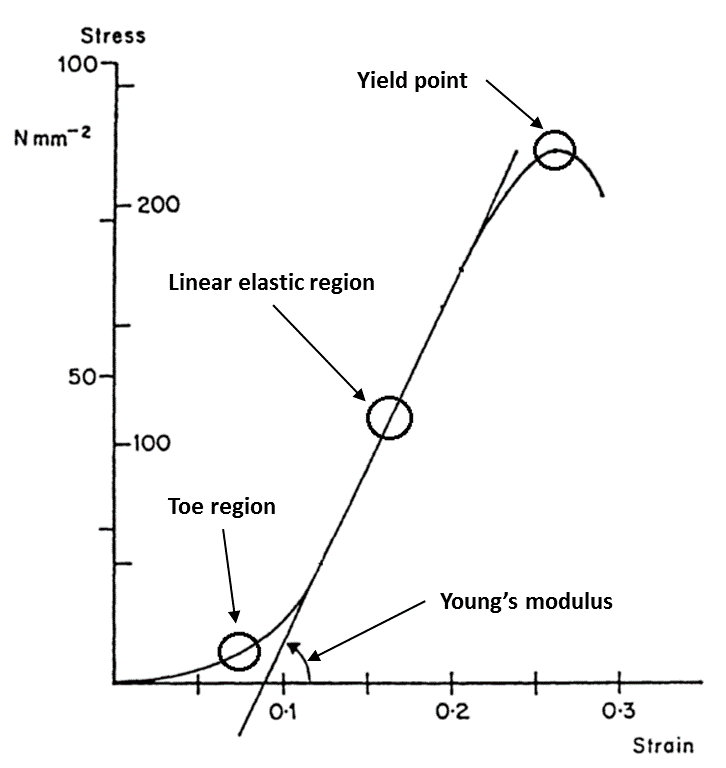
\includegraphics[width=0.6\textwidth]{TendonStressStrain.png}
    \caption{Tendon stress-strain curve. Image adapted from \cite{maurel1998biomechanical}. }
    \label{fig:tendonSS}
\end{figure}

The stress-strain curve in \Cref{fig:tendonSS} illustrates the mechanical properties of a human tendon. The stress is described as the tensile force per cross-sectional unit area experienced by the tendon. This stress causes the tendon to elongate (deform). In the chart, the elongation is represented as the strain, which is the tendon deformation in relation to its original length. Along with the stress-strain curve, the force-elongation curve is also used to visualize the mechanical properties of tendons. These experiments are performed in a static state, i.e. the strain rate is the same throughout the whole experiment. Therefore, they do not provide any information about the viscoelastic properties of the tendon.

Viscoelastic materials exhibit both elastic and viscous characteristics. Viscosity describes a fluid's resistance to flow, the more viscous a fluid is, the more slowly it will flow and vice versa. The latter suggests a time-dependent behaviour. In the case of viscoelastic materials, this time-dependent behaviour is shown when subjecting the material to different rates of strain or deformation. For example, the stress-strain curve of the human tendon, illustrated in \Cref{fig:tendonSS}, would have a greater slope in the elastic region if a greater strain rate is applied. The viscoelastic behaviour of the human tendon can be analysed with the following mechanical tests: stress relaxation, creep (deformation over time) and hysteresis \cite{nordin2001basic}.

During the stress relaxation experiment, the tendon is subjected to a constant deformation (length remains the same throughout the whole experiment). To avoid plastic deformations, i.e. incorrect measurements, the parameter of deformation for this experiment must not exceed the linear region of the material. The initial force/stress triggered as a response of the applied deformation will decrease over time (relax) until reaching equilibrium. From this experiment a chart of force against time is generated (\Cref{fig:tendonSR_Creep}). In a similar way, in the creep experiment a constant force, avoiding plastic deformations, is applied to the material. The material will creep as time passes, in other words, the deformation caused by the applied force will increase over time until reaching equilibrium. A chart of deformation against time is generated (\Cref{fig:tendonSR_Creep}). Finally, during the hysteresis experiment the tendon is subjected to cyclic tests where a load is applied up to a certain stress level and then released (unloading). The tendon behaviour shows two different paths, one for loading and one for unloading. Due to the time-dependent behaviour of viscoelastic materials, each cycle will generate different load-unload paths since the time interval for each cycle to be executed are intentionally defined to prevent the material of reaching equilibrium (\Cref{fig:tendonHysteresis}).

\begin{figure}[htb!]
    \centering
    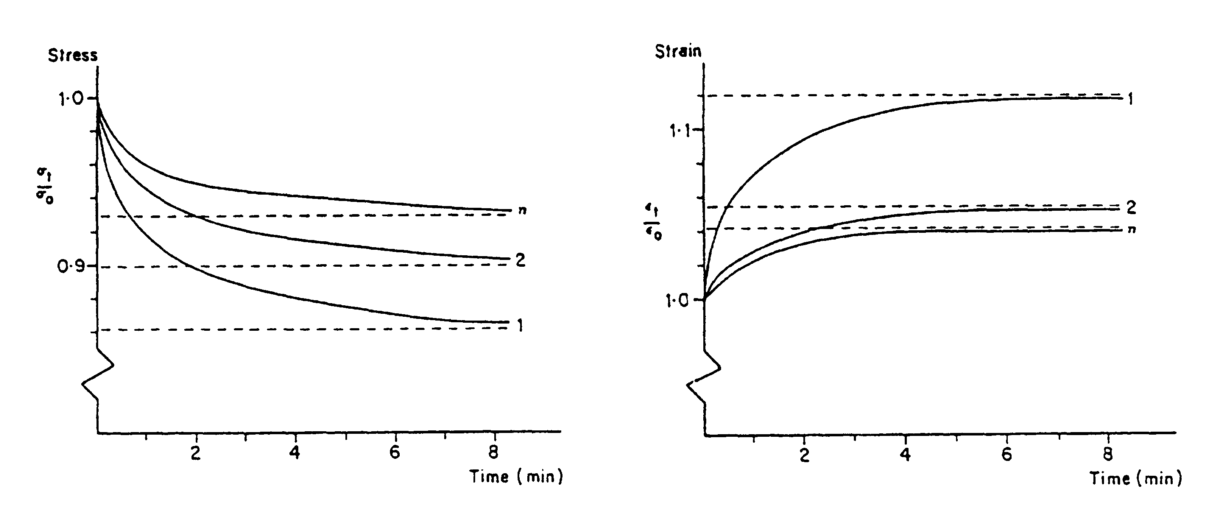
\includegraphics[width=\textwidth]{TendonSR&Creep.png}
    \caption{Tendon curves for the experiments of: (a) stress relaxation and (b) creep. The experiments were executed several times under the same conditions, the curve labelled \textit{n} illustrates the tendon reaching a steady state where repeatability between experiments is achieved. Image reproduced from \cite{maurel1998biomechanical} }
    \label{fig:tendonSR_Creep}
\end{figure}

\begin{figure}[htb!]
    \centering
    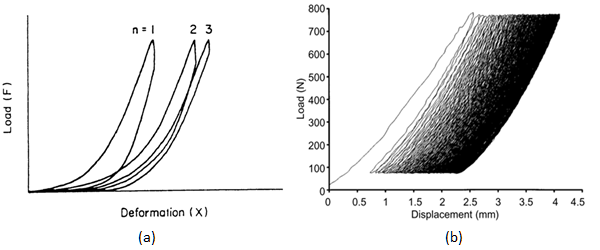
\includegraphics[width=\textwidth]{TendonHysteresis.png}
    \caption{Hysteresis of the human tendon. (a) Deformation chart shows both loading and unloading paths for few cycles and (b) displacement chart shows 200 loading-unloading cycles. The preconditioned state of the tendon is reached for cycles above 50. Images taken from \cite{maurel1998biomechanical,schatzmann1998effect} respectively. }
    \label{fig:tendonHysteresis}
\end{figure}

When performing mechanical experiments to find the tendon properties at failure, the obtained results are different between a preconditioned and an unconditioned tendon, as proved in \cite{schatzmann1998effect}. This effect is illustrated in \Cref{fig:tendonSR_Creep} as well, for both experiments, the tendon relaxation and creep are smaller for each new testing cycle until reaching an equilibrium state, i.e. the preconditioning state. The previous set of experiments is useful to characterize the non-linear viscoelastic properties of tendons and soft materials. Therefore, to perform the comparison analysis mentioned in \Cref{sec:muscle_tendon}, the soft materials of interest must be characterized using some of these mechanical tests. The study of the creep and hysteresis is out of the scope of this research. Instead, the tensile strength and stress relaxation are analysed. The selection criteria for the synthetic soft materials to be used is explained in the next section.

\section{Soft Materials to Match the Properties of the Human Tendon} \label{sec:softMaterials}

The selection of the soft material to be implemented was based on the literature about tendon reconstruction applications. A comprehensive review about the usage of synthetic materials in tendon reconstruction is made by Andullah in \cite{abdullah2015usage}, where the most common materials used as artificial tendons and for tendon reconstruction are reported as: carbon, polyethylene terephthalate (polyester), polytetrafluoroethylene, among others. The latter suggest that polymers are highly compatible with the human skeletal system and have similar mechanical properties as the human tendon. This assumption is further verified in the study performed by Duenwald et al. in \cite{duenwald2009viscoelastic}, which is about the viscoelastic relaxation and recovery of the human tendon. In this work, a high density polyethylene material was tested to find great similarities between this material and the mechanical properties of the human tendon. In fact, the viscoelastic properties of the human tendon during loading and unloading are similar to the ones found in polyethylene. However, high density polyethylene is not able to sustain high strains without suffering plastic deformations nor it has a very fast elastic response.

Among the current developments in soft orthoses, silicone rubber is a common choice, due to its high compliance, high elasticity and softness. Silicone rubber is usually implemented to create inflatable elements, but it is also known to have non-linear elastic properties, as reported in \cite{roylance2008mechanical}. These findings suggest that the limitations of polymers, in terms of their elasticity, could be circumvented when combined with elastomers, such as rubber. A material with the latter characteristics, is known as a composite material. Many composite materials are created by injecting polymer particles, such as the previously mentioned polyethylene, into a rubber mixture. Thanks to the advances in manufacturing of composite materials, there is a wide variety of commercially available materials that fit with the requirements of this research. Due to the latter information, the selection of the soft materials to be studied in this work are from the family of composite materials, as follows: Polyethylene Rubber, Ethylene Polypropylene, Natural Rubber with Polyester, Natural Rubber, Silicone Rubber, Fluorocarbon Rubber, and Nitrile Rubber. All the materials were acquired from RS Components UK\textregistered{}, with the exception of the Natural Rubber, which was acquired from CoreZone Sports\textregistered{} in the form of resistance bands of different thickness. Finally, the characterization process and more details about the materials are provided in \Cref{ch:characterizationSoft}.

\section{Modelling Techniques for Soft Materials} \label{sec:modelingTechniques}

In \Cref{sec:gaps}, the lack of a reliable model to predict the mechanical behaviour of soft materials was identified as a gap in the body of knowledge. This limitation plays a crucial role in the process of investigating the potential benefits of mimicking the human skeletal muscle functionality, and so it is addressed in this section. 

Most of the documented soft robotic applications use soft materials from the family of thermoplastic elastomers (TPE). These type of materials are known to have a non-linear stress response, low stiffness, high deformation lengths, and a time-dependent and temperature-dependent response \cite{Bauman2008}. These mechanical properties are similar to the ones found in biological skin or muscle tissue, which is why soft materials are being implemented in soft robotic applications, despite of the many challenges. However, it is imperative to have a reliable modelling technique to fully take advantage of the latter mechanical properties.

At this point, it has been established the complexity of the mechanical behaviour of soft materials, such as TPE. In general terms, the stress response of these materials is non-linear and viscoelastic. The most commonly modelling technique used when dealing with viscoelastic materials is the development of a mathematical constitutive model. Many authors, choose the Linear Viscoelastic Models (LVM) as the starting point \cite{xu2014mathematical,tirella2014strain,lu2017constitutive,ciniello2017identifying}. This has also been the case when modelling the mechanical behaviour of biological tissues \cite{sanjeevi1982viscoelastic}. The LVM are a set of mathematical models which use two basic components, a spring and a damper, in different configurations and quantities to describe the viscoelastic mechanical behaviour of materials \cite{roylance2001engineering}. Inside this family of mathematical models, there are a couple of them which are considered able to describe the viscoelastic behaviour of any material, as long as the required number of parameters of the model is met. This immediately imposes the restriction of having enough computational power to deal with the model complexity when high accuracy is required.

At this stage of the research, the implementation of soft materials in soft robotic applications for human assistance has gained more attention. Most of the efforts are focused on improving the traditional series-elastic actuator (SEA) by replacing its elastic element, commonly a metallic spring, with a viscoelastic material, such as rubber. SEA are from the family of cable-driven actuators and are commonly based on electric motors. The main feature of these actuators is that they have an elastic element between the actuator and the load. SEA have greatly impacted the field of robotics, specifically in legged robotics and powered orthoses, due to many benefits such as: greater shock tolerance, low output impedance, passive energy storage, and better force feedback accuracy \cite{pratt1995series,pratt2004series,au2008powered}. Almost two decades after Pratt et al. documented the first SEA prototype, SEA are now considered a mature actuation technology, and as such, they have a well-defined trade-off, caused by the fixed stiffness provided by linear springs traditionally used. More often than not, variable stiffness is more suitable for legged robots and powered orthoses. The latter limitation have been addressed by developing variable stiffness actuators \cite{groothuis2012vsaut}, using non-linear metallic springs \cite{migliore2007novel}, and very recently by using viscoelastic materials, such as polymers and rubber \cite{rollinson2013design,parietti2011series,schepelmann2014compact}. However, these works, specifically the ones dealing with soft materials, are still facing the challenge of modelling the mechanical properties of this type of materials. 

In \cite{parietti2011series}, where the concept of a series-viscoelastic actuator (SVA) is first mentioned, the modelling of the soft material is based on the Burger Model, one of the most complete LVM, in combination with a controlling technique known as the state space observer. The accuracy of the system was found to be proportional to the complexity of the mathematical model used. The studied material in this work was a rigid-acrylic based photopolymer (FullCure720). The reported control system contained the viscoelastic model, the state space observer, and a cascaded force-velocity scheme, in other words, a very complex and well thought control system for a linear viscoelastic polymer. The developed SVA is illustrated in \Cref{fig:firstSVA}. 

\begin{figure}[htb!]
    \centering
    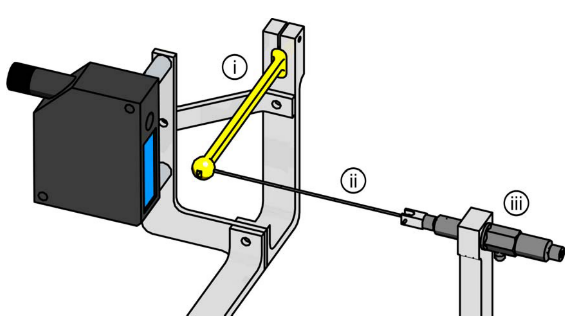
\includegraphics[width=0.6\textwidth]{FirstSVA.png}
    \caption{Series-viscoelastic actuator proposed by Parietti et al. The end effector is rigidly mounted on the revolving lever (i), which also supports the laser sensor. A Nylon line (ii) connects the end-effector handle to the high-precision piezoelectric force sensor (iii), which is fixed to a rigid support \cite{parietti2011series}.}
    \label{fig:firstSVA}
\end{figure}

Following this line of research, Rollinson et al. attempted to add viscoelasticity to a SEA, this time a soft material is used, natural rubber, instead of a rigid polymer \cite{rollinson2013design}. The developed SEA has a rotary spring. Two different types of rubber, and a type of neoprene, were studied. In here, the stress response of the materials is considered linear and instead, the hysteresis of the material is modelled. Again, the modelling of the soft material is based on one of the LVM, the Standard Linear Solid (SLS) model, which is slightly less complex than the Burger model. Thanks to the proposed mechanical design for the rotary SEA, the reported stress response of the studied rubbers was surprisingly linear under a specific range of deformations. The authors concluded that more work is required to create better modelling techniques for the hysteresis and non-linear behaviour of soft materials like elastomers. The developed rotary spring is illustrated in \Cref{fig:rotarySoftSEA}.

\begin{figure}[htb!]
    \centering
    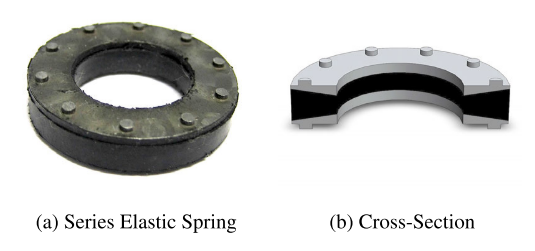
\includegraphics[width=0.6\textwidth]{RotarySoftSEA.png}
    \caption{Developed soft rotary spring: a)photo and b)cross-section \cite{rollinson2013design}.}
    \label{fig:rotarySoftSEA}
\end{figure}

Following a more traditional approach, Schepelmann et al. incorporated viscoelasticity in cable-driven SEA by using a rubber material as the elastic element, instead of the traditional metallic spring \cite{schepelmann2014compact}. In here, no LVMs are used, instead the non-linear stress response of the rubber is simplified by fitting a second order exponential curve to the stress-strain curve of the material. The main motivation of this work is to tackle the limitations of SEA with non-linear springs (NLS), where computer-aided manufactured (CAM) structures are used to define a known deflection trajectory of the spring, thus defining a torque trajectory. Essentially, CAM structures are able to relate the spring deformation with the generated torque, allowing the implementation of control systems. This work successfully validated the suitability of rubber to be incorporated as part of a SEA (\Cref{fig:softSEACAM}). However, under the limited range of testing parameters, the authors were not able to observe any velocity-dependency on the stress response of the rubber. In the conclusions, a state space observer is recommended to improve the accuracy of the reported forces transmitted by the the soft material, i.e. to allow the controller to compensate the hysteresis and non-linear stress response of the material.

\begin{figure}[htb!]
    \centering
    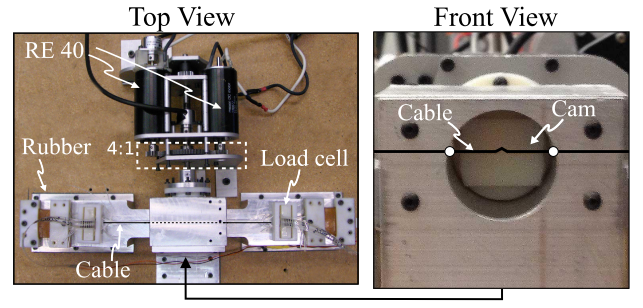
\includegraphics[width=0.6\textwidth]{SoftSEACAM.png}
    \caption{Benchtop setup for rubber characterization and observer testing. The load side of the rubber is fixed. Load cells in-line with the rubber give rubber force measurements for testing. The choice of electric motors and transmission is illustrated \cite{schepelmann2014compact}}
    \label{fig:softSEACAM}
\end{figure}

In an attempt to relieve the controller for such load, the latter work was continued by Austin et al. in \cite{austin2015control}, this time the focus was on developing a modelling tool to better model the complex behaviour of rubber. In here, the complexity of modelling the non-linear and strain-dependent stress response of soft materials is addressed, for the first time, by upgrading the SLS model without greatly increasing its complexity. A piecewise linearization method is implemented, to transform the equilibrium spring in the SLS model into several springs in parallel which sequentially engages in proportion to the strain applied to the material. The developed mathematical model is called the Standard Linear Solid model with Strain-Dependent Stiffness. (Std. Lin. SDS). Although, the SLS is not the most complete model among the LVM, the reported accuracy of the developed model is impressive. The control system implemented a state space observer, as well, which was able to correctly estimate the torque generated by the rubber spring. However, despite the large improvement in accuracy obtained by the developed Std. Lin. SDS, the hysteretic properties of the rubber  lead to instability at higher frequencies, suggesting that there is still work to be done in this field.

\section{Summary}

In this chapter, the terminology on the biomechanics of the human lower limb is presented. Subsequently, the characterization of the kinetic and kinematic parameters of the hip, knee and ankle joints is performed by reviewing many clinical trials about gait analysis of the lower limb. The collected data had the potential to be used as design guidelines when developing robotic devices targeted for human assistance. Therefore, many visualization techniques were proposed and analysed in this context. The latter work resulted in a published conference paper (\Cref{sec:characterizationKKP}). 

The main element of the human skeletal muscle system, the muscle-tendon component, was described in \Cref{sec:muscle_tendon}. In the literature, the works that implement the concept of mimicking the muscle skeletal system are focused on the contractile element of the muscle-tendon component, i.e. the muscle. Very little attention is paid to the series element, the tendon. Furthermore, it was found that the viscoelasticity present in the human tendon, and biological tissues in general, is also present in certain polymers and composite materials. Therefore, the proposal of performing a comparison analysis between different off-the-shelf composite materials and the human tendon mechanical properties is presented. This comparison analysis will contribute to the aforementioned aim of the research. The first step to perform this comparison analysis is to characterize the mechanical properties of the selected materials, listed in \Cref{sec:softMaterials}. This is described in \Cref{ch:characterizationSoft}.

Recently, attempts of adding viscoelasticity to well-established actuation technologies have been done. Specifically, viscoelasticity has the potential to address many of the limitations found in series-elastic actuators. The available literature on the subject is scarce but very well documented. In general, the reviewed works face a common challenge, the modelling of the viscoelastic properties of the materials used to accurately estimate their reaction force or torque. Rubber is the most common choice in these applications. Almost all of the documented works are based on a model-driven approach, based on the Linear Viscoelastic Models, for the prediction of the material behaviour. However, the work performed by Austin et al. in \cite{austin2015control}, is the first attempt to upgrade the potential of the LVMs by applying a piecewise linearization method. The authors succeeded in developing a mathematical model, called the Standard Linear Solid model with Strain-Dependent Stiffness. (Std. Lin. SDS) which achieved higher accuracy than traditional models. However, even with the aid of controlling techniques such as the state space observer, the implemented control system is still unable to account for properties of the material, such as hysteresis and the velocity-dependency in their stress response. Nevertheless, the developed mathematical model has the potential to be upgraded further by using the same piecewise linearization method but on a more complex LVM. This idea is further explored in an attempt to develop a reliable modelling tool for the prediction of the mechanical properties of soft materials. This is presented in \Cref{sec:ChapterModellingLVM}.



\chapter{Characterization of the Mechanical Properties of Soft Materials} \label{ch:characterizationSoft}

\section{Introduction}

In the previous chapter, the trend in soft robotic applications for human assistance of mimicking the human skeletal muscle system was identified. This trend is mainly focused on the contractile element (CE) of the muscle-tendon component. Recently, research has been done on implementing soft materials as the elastic element of series-elastic actuators (SEAs). This is motivated by the fact that viscoelasticity, found in biological tissue and many soft materials, may be able to overcome current limitations on SEAs. This is inline with the literature, which states that polymers, such as polyethylene, have similar mechanical properties as the human tendon. The literature available on the concept of series-viscoelastic actuators (SVAs) is very scarce and is currently facing the challenge of accurately estimating the force/torque transmitted by soft materials, such as rubber. One of the aims of this research is to develop a modelling tool able to address the latter. Therefore, this chapter covers the following points.

Firstly, a selection of different off-the-shelf soft materials is made from the family of composite materials, specifically thermoplastic elastomers (TPEs). The selection is based on the literature, which suggest that this type of materials have similar viscoelastic properties as the human tendon. The materials are as follows: Polyethylene Rubber (PR), Ethylene Polypropylene Rubber (EPR), Natural Rubber with Polyester (NatPolR), Natural Rubber (NatR), Silicone Rubber (SR), Fluorocarbon Rubber (FR), and Nitrile Rubber (NR). All the materials were acquired from RS Components UK\textregistered{}, with the exception of the Natural Rubber, which was acquired from CoreZone Sports\textregistered{} in the form of resistance bands of different thickness.

Secondly, the mechanical property of viscoelasticity of this type of materials is discussed. Thirdly, the characterization of the mechanical properties of these materials is presented. In here, the mechanical tests of tensile strength and stress relaxation are performed to extract both the elastic and viscoelastic properties of the materials. As previously mentioned, the study of the creep and hysteresis effect is out of the scope of this research. Finally, the collected data was processed in Matlab\textregistered{} prior to creating the visual representation of the studied properties. 

\section{Mechanical Properties of Soft Materials} \label{sec:mechprop}

The soft materials studied in this work belong to the family of thermoplastic elastomers or TPE. These materials are created by mixing a thermoplastic material, such as natural or synthetic rubber, with other materials, such as carbon and sulfur. This process is called vulcanization which creates cross-linked structures inside the material. Since elastomers are based on rubber, the terms elastomer and rubber are often used interchangeably. Elastomers are known to have nonlinear stress response, low stiffness and to achieve high deformation lengths. Some elastomers can fully recover their shape after stretched many times their length. They are also known to exhibit both elastic and viscoelastic properties. The latter means the stress response of elastomers is also time-dependent \cite{Bauman2008}. The main mechanical properties of elastomers are described in following paragraphs.

\subsection{Elasticity}

Elasticity, or elastic behaviour, refers to the ability of a material to be deformed up to a certain length and completely recover its shape and dimensions when the load deforming it is removed. Elasticity also refers to ability of a material to comply with the law of constant proportionality between the stress and the strain, described by Hooke's Law. However, elastomers are not purely elastic materials and tend to have a nonlinear stress-strain response, i.e. they do not obey Hooke's Law over the whole range of strains in the sense that the proportionality between the stress and the strain does not remain constant. This typical nonlinear behaviour in the stress-strain curve of elastomers is illustrated in \Cref{fig:tensile}.

\begin{figure}[hbt!]
    \centering
    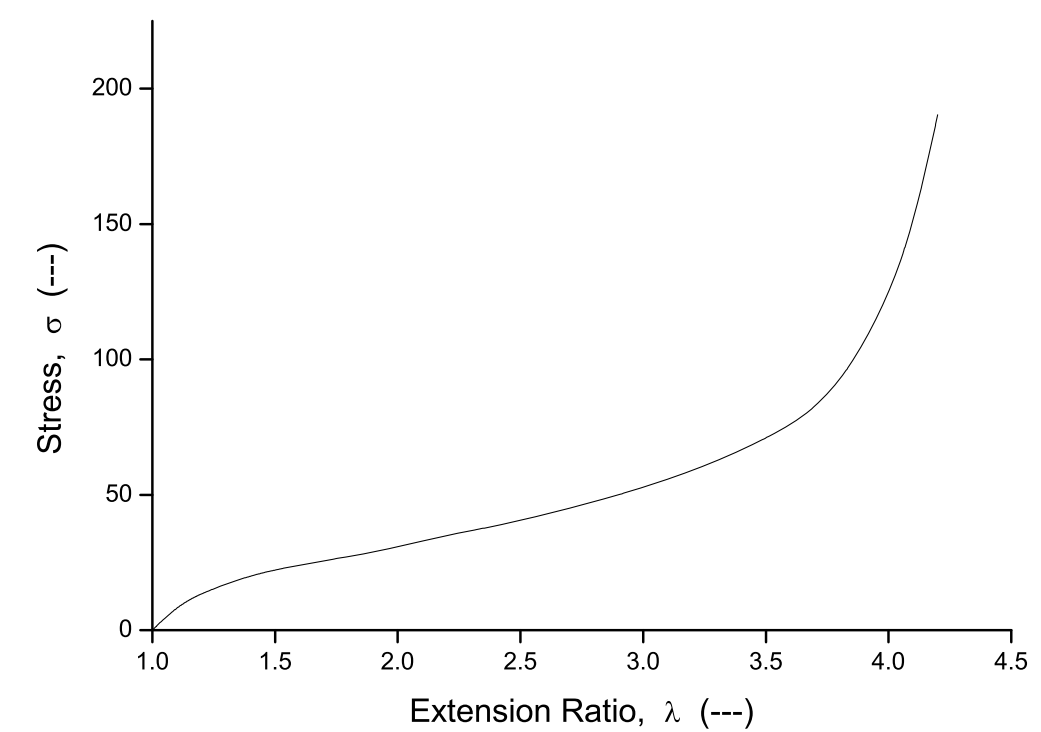
\includegraphics[width=0.6\textwidth]{TensileExample.png}
    \caption{Typical stress-strain curve of elastomers. There are three main regions: the toe region (1.0 < $\lambda$ < 1.5), the elastic region (1.5 < $\lambda$ < 3.5), and the yield/failure region ($\lambda$ > 3.5) \cite{Bauman2008}.}
    \label{fig:tensile}
\end{figure}

The stress-strain curve of elastomers, illustrated in  \Cref{fig:tensile}), has three main regions: the toe region (1.0 < $\lambda$ < 1.5), the elastic region (1.5 < $\lambda$ < 3.5), and the yield/failure region ($\lambda$ > 3.5). In the toe region, the internal molecular chains of the material are misaligned, experiencing greater friction forces which greatly oppose to initial deformations. In contrast, when the molecular chains are aligned the friction forces decrease and the material deforms as a whole. The latter conditions dictates the beginning of the elastic region, in which the slope of the curve (stiffness) is slightly smaller than in the toe-region. The elastic region of many materials exhibit a proportional or linear relationship between the stress and the strain. This is not the case for elastomers, where most of them exhibit a nonlinear relationship. When the internal molecular chains have been elongated to its maximum length they demand higher forces to fail, this is observed as a peak in the load-elongation curve which also highlights the beginning of the yield/failure region \cite{Bauman2008}.

Elastomers exhibit elastic behaviour over a certain range of deformations, i.e. the elastic region or elastic limit. Beyond this limit the material is likely to undergo plastic or permanent deformation, this means the material will not recover its original shape completely. In some cases, the elastic limit is not easily visible on the stress-strain curve of a material, and instead the proportional limit is used to approximate the location of the elastic limit. The proportional limit is defined as the point in the stress-strain curve where the nonlinear response (change in the curve's slope) is first observed. Another way to approximate the elastic limit of a material is based on using the yield strength, which is defined as the largest stress value on the curve, or the first point in which an increase in strain occurs without an increase in the stress \cite{ebewele2000}. These are some of the parameters that can be extracted from the tensile strength test and are useful to delimit the operating conditions of the materials. For this reason, particular care is put into accurately defining the elastic region, hence the safe operating conditions, of the studied soft materials. This is better described in \Cref{sss:elasticProperties}.

\subsection{Viscoelasticity}

Viscoelasticity, is a property of some materials which are not purely elastic, do not fully obey Hooke's Law, nor purely viscous, do not fully obey Newton's Law, i.e. the stress is not proportional to the rate of change of the strain with time. In other words, the stress experienced by viscoelastic materials are dependent on both the amount and the speed of the strain applied to them. An example of a purely elastic material is a spring; whereas an example of a purely viscous material is a dashpot. The mechanical model of a viscoelastic material contains both elements, which can be arranged in different configurations. The set of mathematical models created out of these different configurations are known as the Linear Viscoelastic Models (LVMs). The time dependency or viscosity, of viscoelastic materials is appreciated in phenomena such as creep, stress relaxation, hysteresis, the Mullin's Effect and in the Van der Waals forces.

Stress relaxation and creep are both time-dependent phenomena observed in elastomers. On the one hand, stress relaxation refers to the decrease over time of the stress experimented by a material when subjected to a constant strain (or deformation). On the other hand, creep refers to the increment over time of the material strain when subjected to a constant stress (or load). The latter phenomena is observed in elastomers because they are composed of an internal network of molecular chains. Inside this network, entanglements form naturally. According to J. Bauman in \cite{Bauman2008}, stress relaxation is mainly caused by the slipping of these entanglements ultimately causing a loosening of force applied by the network of molecular chains. Stress relaxation and creep occur in both constant and cyclic deformations. There are two mechanical tests designed to study these behaviours, from where the relaxation modulus and creep modulus of a material can be extracted \cite{oberg2016}. 

Hysteresis in a material is defined as the mechanical energy dissipated as heat when the material is undergoing deformations. This phenomenon is observed in a loading-unloading cycle, where the stress trajectory of the material while loading (extension) is different than the trajectory during unloading (retraction), as illustrated in \Cref{fig:hysteresis}. Hysteresis is mainly caused by internal friction of the molecular chain, also known as Van der Waals forces, in both elongation and contraction. Van der Waals forces are caused by the momentary bonding experienced between molecular chains that are close together. This constant making and breaking of bonds caused by deforming a material produces heat which ultimately becomes a mechanism to dissipate mechanical energy. This energy is represented as the enclosed area in \Cref{fig:hysteresis}. Stress relaxation and creep play a role in the amount of hysteresis experienced by a material in each consecutive loading-unloading cycle. The effect of hysteresis alone can be isolated by subjecting the elastomer to a conditioning process (preconditioning) in which it undergoes several loading-unloading cycles until the stress response stops changing with every new cycle.

\begin{figure}[htb!]
    \centering
    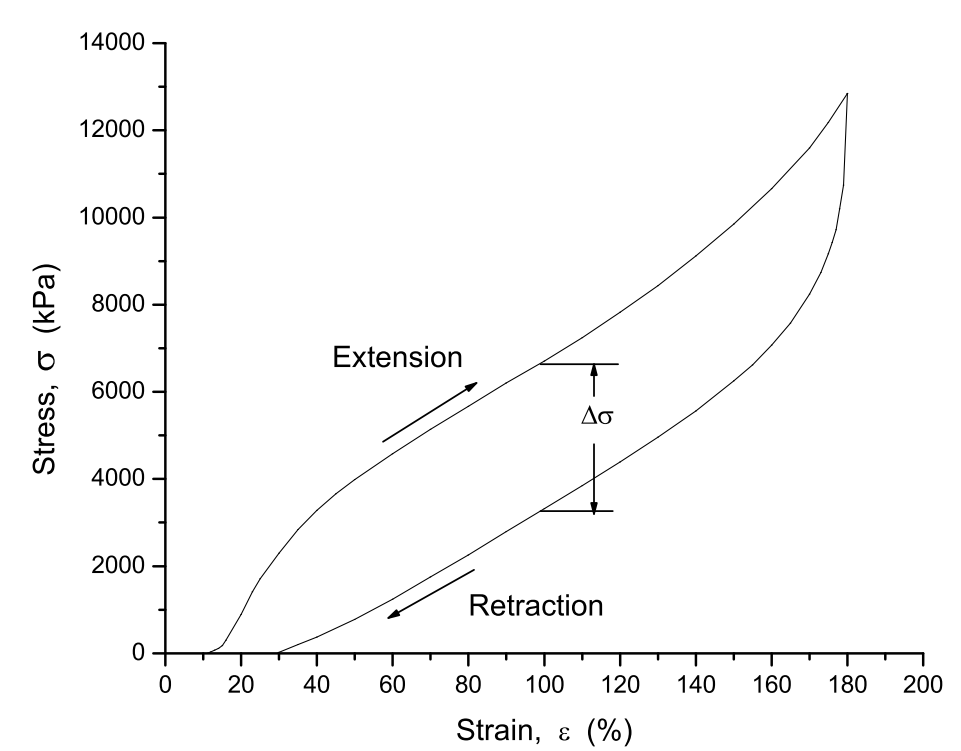
\includegraphics[width=0.8\textwidth]{HysteresisExample.png}
    \caption{Hysteresis in stress-strain curve. \cite{Bauman2008}.}
    \label{fig:hysteresis}
\end{figure}

The Mullin's effect is another important phenomenon in the mechanical behaviour of elastomers. This effect refers to the breakage of tense molecular chains resulted from the manufacturing process of the material. Therefore, the very first time the material is subjected to deformations it exhibits a larger stress response in comparison to consecutive deformations. The latter is also referred to as a weakening of the material. This effect is more dramatic than the stress relaxation but can be easily avoided when preconditioning the material. Having defined the expected mechanical properties of elastomers, the mechanical tests of tensile strength and stress relaxation are described in the following section.

\section{Characterization Process} \label{sec:CharacterizationProcess}

In this section, the mechanical tests of tensile strength and stress relaxation, performed as part of the characterization process, are described. The tests are performed in an Instron 3369 Dual Column Testing System equipped with a 50 kN load cell, at room temperature (25 \degree{} C). The experimental data is expected to contain some noise due to the accuracy limitations of the available load cell. The algorithm implemented to filter this noise is described in \Cref{sss:dataProcessing } . As previously mentioned, the elastomers selected for this research are: Polyethylene Rubber (PR), Ethylene Polypropylene (EPR), Natural Rubber with Polyester (NatPolR), Natural Rubber (NatR), Silicone Rubber (SR), Fluorocarbon Rubber (FR), and Nitrile Rubber (NR). The Natural Rubber material is acquired from CoreZone Sports\textregistered{} and comes in the form of resistance bands of different thickness. The other materials are acquired from RS Components UK\textregistered{}, and come in the form of a rectangular sheet form. Laser cutting was used to extract individual specimens from each material sheet with the layout illustrated in \Cref{fig:specimenLayout}, as recommended in the Standard Test Method for Vulcanized Rubbers - Tension (ASTM D412) \cite{astmd412}. Finally, all the specimens were preconditioned prior to testing by applying a small deformation to them.

\begin{figure}[htb!]
    \centering
    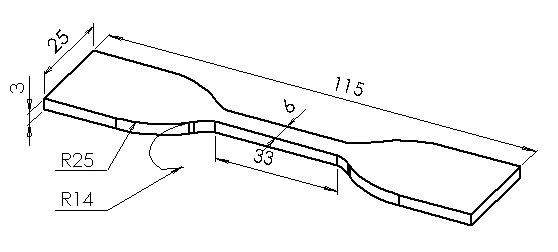
\includegraphics[width=0.6\textwidth]{SpecimenLayout.png}
    \caption{Specimen Type C Dumbbell Layout from the ASTM D412 \cite{astmd412}. In this example, the specimen thickness is 3mm, the width is 6mm, and the initial length, $l_o$, is 33mm.}
    \label{fig:specimenLayout}
\end{figure}

\subsection{Tensile Strength Test}

In a tensile strength test the material is loaded to failure at a certain deformation (strain) rate. The main purpose of this test is to extract the stress-strain curve of the material. From the stress-strain curve, the elastic properties of the material, such as stiffness, elastic modulus, ultimate strain, ultimate stress, elastic limit and yield strength, can be extracted. 

The tensile strength test performed in this work is in accordance with the Standard Test Method for Vulcanized Rubbers - Tension (ASTM D412) \cite{astmd412}. Also, the Standard Test Method for Tensile Properties of Plastics (ASTM D638), was consulted on how to interpret the obtained stress-strain curves \cite{astmd638}. In here, it is recommended to elongate the material specimen until failure using a deformation rate of 500 mm/min, whenever possible. However, under certain circumstances where the previous deformation rate is not suitable, the test can be performed using the deformation rate of 250 mm/min. The latter was required for the silicon rubber, natural rubber and some resistance bands, where the gripper of the testing machine was not able to hold the material during the entirety of the test. In addition to the previous two deformation rates, a third one of 50 mm/min is used whenever possible. In summary, most of the materials are tested using at least two out of the three deformation rates of 50, 250 and 500 mm/min. The decision of characterizing the mechanical behaviour of the materials under different strain rates is motivated by the known velocity-dependency of the stress-response of this type of materials. This will be useful during the modelling stage. The exact number of tests performed to each material is summarized in \Cref{tbl:tensile_tests}. 

\begin{table}[htb!]
    \centering
    \caption{Number of specimens used per type of test}
    \begin{tabular}{lcccc}
    \toprule
    Type of Rubber & Thickness &  50 & 250 & 500\\
     & mm & mm/min & mm/min & mm/min \\
    \hline
    Ethylene Polypropylene   	&  1.5 & 16 & -- & 5\\
    Fluorocarbon              	&  1.5 & 8 & 8 & 5\\
    Natural with Polyester   	&  1.5 & 11 & 5 & 1\\
    Nitrile                   	&  1.5 & 8 & 7 & 6\\
    Silicone                  	&  1.5 & 15 & 7 & --\\
    Polyethylene              	&  6 & 13 & 7 & 1\\
    Natural (Resistance Bands)	& 0.33 -- 1.49 & 1 & 33 & 11\\    
    \bottomrule
    \end{tabular}
    \label{tbl:tensile_tests}
\end{table}

The testing machine used for these experiments output the following parameters: reaction force, elongation, and time. In this work, the conventional parameters of stress, $\sigma$, and strain, $\varepsilon$, are used instead of the reaction force, $F$, and elongation, $\Delta L$. The latter is calculated using the initial length $l_o=33 mm$, and cross-sectional area $A_o$, of the specimen, illustrated in \autoref{fig:specimenLayout} and \autoref{tbl:tensile_tests}, respectively. Then it follows that $\sigma=F/A_o$, and $\varepsilon$=$\Delta L$/$l_o$.

\subsubsection{Data Processing} \label{sss:dataProcessing}

The main objective of the data processing stage is to get rid of any noise added to the experimental data, normally due to sensor limitations, and also to filter out any undesired data. Removing noise from the data, i.e. filtering or smoothing, is avoided whenever possible because meaningful data can be lost in the process. Unfortunately, some of the collected datasets showed signs of high frequency noise which make it vary rapidly. A smoothing algorithm was applied to these datasets. In addition to noise, there are two sections of the collected stress-strain curve which are not desired. The first one is the section of the curve beyond the failure point of the material, when the stress value precipitates to zero. The working conditions of the soft material are desired to be limited to its elastic region, therefore, the final section of the stress-strain curve is not critical for the modelling of the materials behaviour. The second undesired section of the stress-strain curve is located at the very beginning. According to the literature, the very first portion of the stress-strain curve can be contaminated with phenomena such as: take-up of slack, and seating of the specimen. This effect was observed for most of the studied materials in here. The process of how to get rid of this phenomenon is called toe compensation (for a detailed description, refer to \cite{astmd638}). The mentioned sections are illustrated in \Cref{fig:rawData}.

\begin{figure}[htb!]
    \centering
    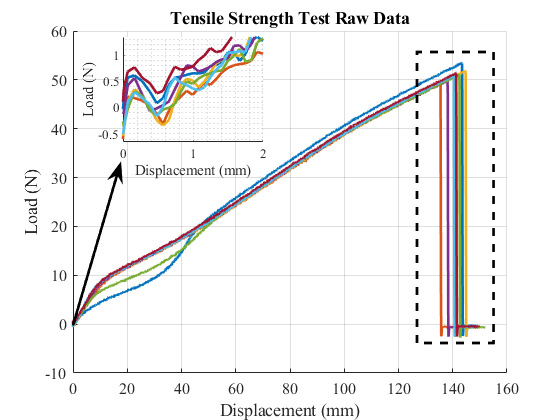
\includegraphics[width=0.9\textwidth]{RawDataToeCompensation.png}
    \caption{Undesired data on the tensile strength results. On the top left, the take-up slack phenomenon at the beginning of the experiment is observed. On the right, the different failure points of each specimen from the same material are highlighted.}
    \label{fig:rawData}
\end{figure}

The stress-strain curve from different specimens of the same material is expected to be slightly different, as illustrated in \Cref{fig:rawData}. This variability is caused by many reasons such as the manufacturing process, temperature, and micro fissures inside the material due to handling. For this reason, and as recommended in \cite{astmd638,astmd412}, the engineering ultimate values of stress $\sigma_{ue}$ and strain $\varepsilon_{ue}$ are reported as the median value from all the tests involving one material and one strain rate. This variation has an impact on the unification of the data performed by averaging the values from all the tests. The latter will yield a single stress-strain curve from all the specimens involved in a test. This is required for the modelling process. In \Cref{fig:unevenData} this impact is illustrated in the form of abrupt changes  around the end section of the curve, caused by the different failing points of each specimen. The presence of this variation is not critical for the modelling stage because the material is unlikely to be elongated to such high lengths in a real wearable robotic application. However, the decision of discarding this section of the curve in favour of calculating the mean ultimate values of stress $\sigma_u$ and strain $\varepsilon_u$, was made. This section of the curve was also not included when generating the final stress-strain curves of the materials.

%%%%%%%%%%%%%%%%
\begin{figure}[htb!]
    \centering
    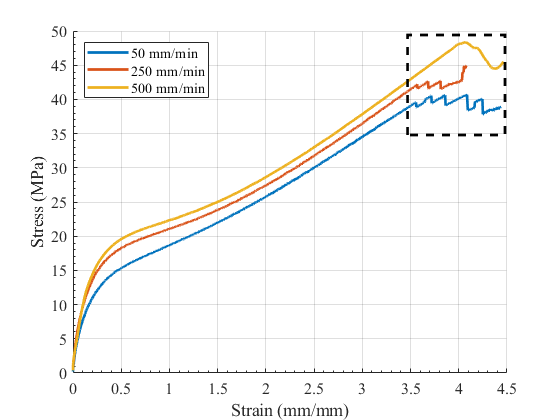
\includegraphics[width=0.7\textwidth]{UnevenUnifiedData.png}
    \caption{Abrupt changes observed at the last portion of the stress-strain curve, caused by the different failure points for each specimen. This phenomenon is observed after unifying the data from all individual specimens of a specific strain rate, into a single stress-strain curve.}
    \label{fig:unevenData}
\end{figure}
%%%%%%

The processing algorithm, developed in Matlab \textregistered{}, was applied to the datasets that exhibit large amount of noise. These datasets were identified by looking at positive and negative peaks, specifically by looking at the mean absolute difference (MAD). Any dataset with peaks having a MAD greater than zero was considered noisy and subsequently filtered out. The filtering of the noise was done using the \texttt{smoothdata} function with the Savitsky-Golay algorithm. This function requires a window parameter to which the smoothing algorithm is applied, the larger the window, the greater the smoothing. However, a large window size also introduces a bias or offset to the extreme points of the data. This trade-off is described in \cite{sadeghi2018optimum}. Due to this, the chosen window size was based on the amount of data contained in one second in this way the window size depends on both the strain rate and the sampling frequency for each case. 

The implemented data processing is summarized as follows:
 \begin{enumerate}[noitemsep] %Requires package enumitem
    \item Load raw data from tensile strength tests, i.e. elongation and reaction force (load);
    \item Discard section of the stress-strain curve beyond the failure point;
    \item Extract engineering ultimate load and displacement, latter converted to stress and strain.
    \item Discard take-up slack phenomenon;
    \item Unify processed data from all specimens into a single dataset by calculating the mean value;
    \item Smooth datasets which have a peak-to-peak MAD greater than zero, in the initial portion of the curve;
    \item Discard negative offset induced by processing and smoothing;
    \item Calculate $\sigma = F/A_o$, and $\varepsilon=\Delta L/l_o$ .
\end{enumerate}

\subsubsection{Elastic Properties of the Material} \label{sss:elasticProperties}

One of the main parameters to extract from the stress-strain curves of the materials is the elastic limit of each material. As previously mentioned in \Cref{sec:mechprop}, this parameter dictates the maximum amount of deformation a material can sustain without losing the ability to fully recover its original shape. Commonly, the proportional limit is used to approximate the location of the elastic limit, and by extension, the elastic region. The proportional limit is the point in the curve where the proportionality between stress and strain becomes nonlinear. It can be safely assumed that the elastic region of the material is located below this point. However, most elastomers do not have a clear elastic region due to their nonlinear stress-strain curve, hence the proportional limit cannot be obtained. Under this circumstance, the elastic region of the material can be approximated using the yield strength of the material. The latter is defined as the first point in the curve where an increment in strain happens without an increment in the stress, in other words when the slope becomes zero or even negative \cite{astmd638}. The yield strength is inside the region of plastic deformations of the material, hence this parameter by itself is not a safe way to approximate the elastic region. 

A better alternative to approximate the elastic region is the offset yield strength. This parameter requires an offset strain value, and the elastic modulus $E$ (slope of the curve) at a specific strain, to be calculated. In the literature, an offset strain of $\varepsilon_{offset}=0.02$, or 2\%, is recommended for plastics and elastomers \cite{instron2019}. This recommendation is mainly to allow comparisons between different laboratories data and does not indicate a goodness of fit when approximating the elastic region or the yield point of a material. In here, we chose a $\varepsilon_{offset}=0.2$, or 20\%, due to the large values of elongation achieved by most of the materials. The main recommendation to calculate $E$ is to choose a strain range inside the initial part of the stress-strain curve in which a linear behaviour can be observed. The elastic modulus is then approximated using a function fitting method such as linear regression. Therefore, the optimal strain range for $E$ was extracted from the obtained stress-strain curves of the materials illustrated in \Cref{fig:EPR-FRSS,fig:NatR-NRSS,fig:PR-SRSS,fig:Nat100RSS}.

In \Cref{fig:EPR-FRSS,fig:NatR-NRSS,fig:PR-SRSS,fig:Nat100RSS}, the stress-strain curve of all the materials studied under different strain rates are presented. The process to obtain the stress-strain curve of the Natural Rubber material was longer than for the other materials, due to the different available thicknesses. This material was acquired in the form of resistance bands, commonly used for rehabilitation. A total of two different batches were acquired. Each batch contained one band for each strength level, a total of six levels. The weakest band was the tinniest, whereas the strongest band was the thickest. The measured force response of one band from the same strength level varied from one batch to the other. The measured thicknesses were not the same among the two batches for a band of the same type. This is directly related to manufacturing practices and is reported in the literature \cite{case2015soft}. For this reason, the individual thickness of each type of rubber band, from each batch was used to convert the raw data to the final stress-strain curve. With this, the impact from the latter differences is decreased and the material behaviour was better captured.
%%%%%%%%%%%%%%%%%%%%%%%%%%%%%%%%%%%%%%%%%%%%%%%%%%%%%%%%%%%%%%%%
\newpage
\begin{figure}[H]
\vspace{-2em}
    \centering
        \begin{subfigure}[b]{0.93\textwidth}
        \centering
        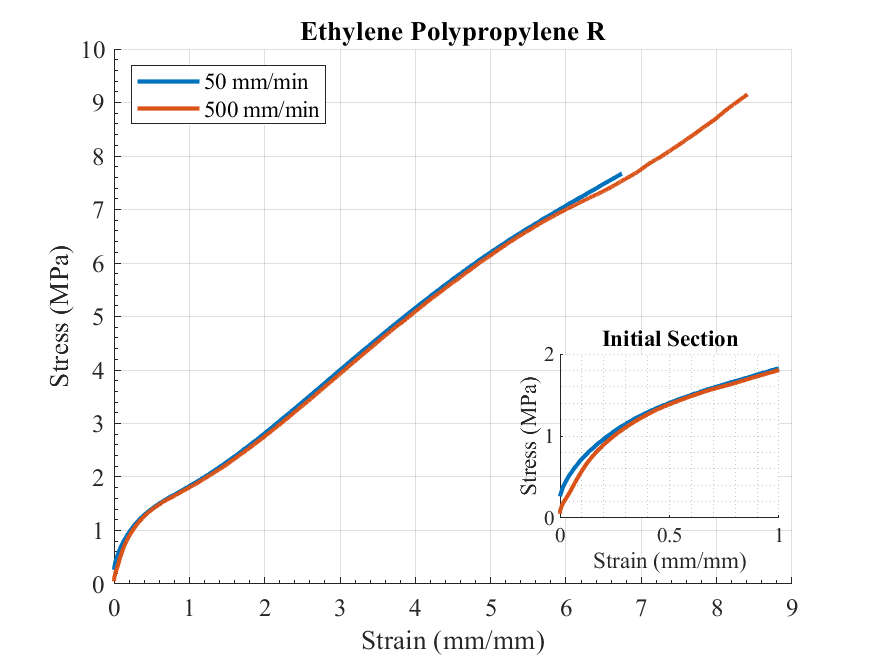
\includegraphics[width=\textwidth]{EPR_StressStrain.png}
        \caption{}
        \label{sfig:EPRSS}
    \end{subfigure}
    \begin{subfigure}[b]{0.93\textwidth}
        \centering
        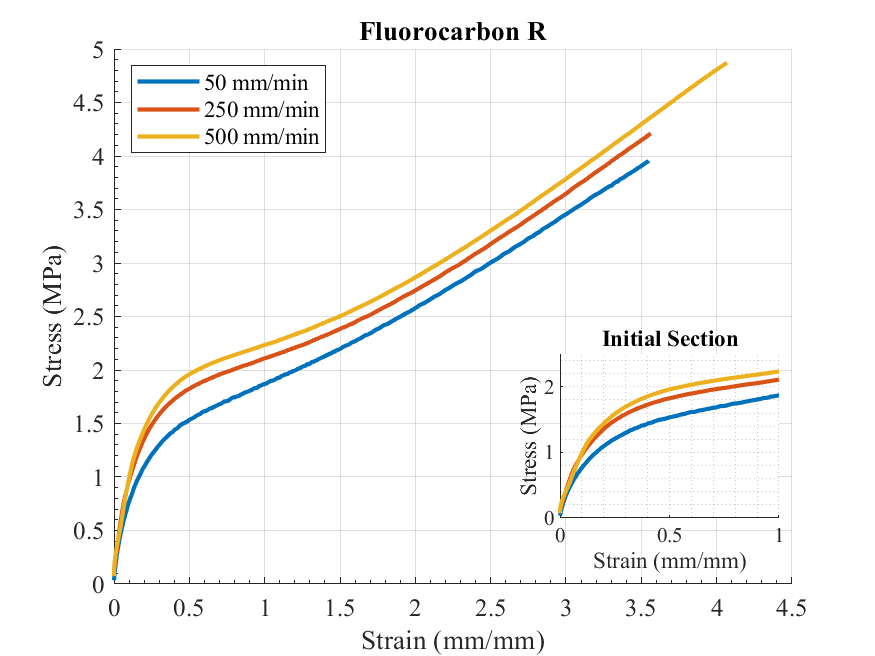
\includegraphics[width=\textwidth]{FR_StressStrain.png}
        \caption{}
        \label{sfig:FRSS}
    \end{subfigure}
    \caption{Stress-strain curves, during different strain rates, for the (a) EPR and (b) FR materials. On the bottom right, the initial section of the curve, where a linear behaviour was observed, is presented.}
    \label{fig:EPR-FRSS}
\end{figure}
\newpage
\begin{figure}[H]
    \vspace{-2em}
    \centering
    \begin{subfigure}[b]{0.93\textwidth}
    \centering
    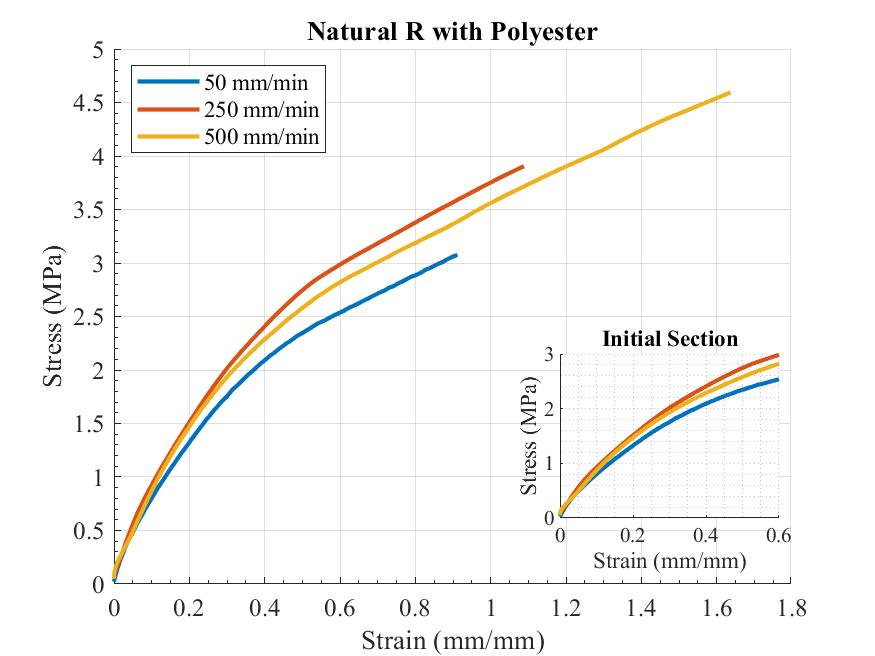
\includegraphics[width=\textwidth]{NatR_StressStrain.png}
    \caption{}
    \label{sfig:NatRSS}
    \end{subfigure}

    \begin{subfigure}[b]{0.93\textwidth}
    \centering
    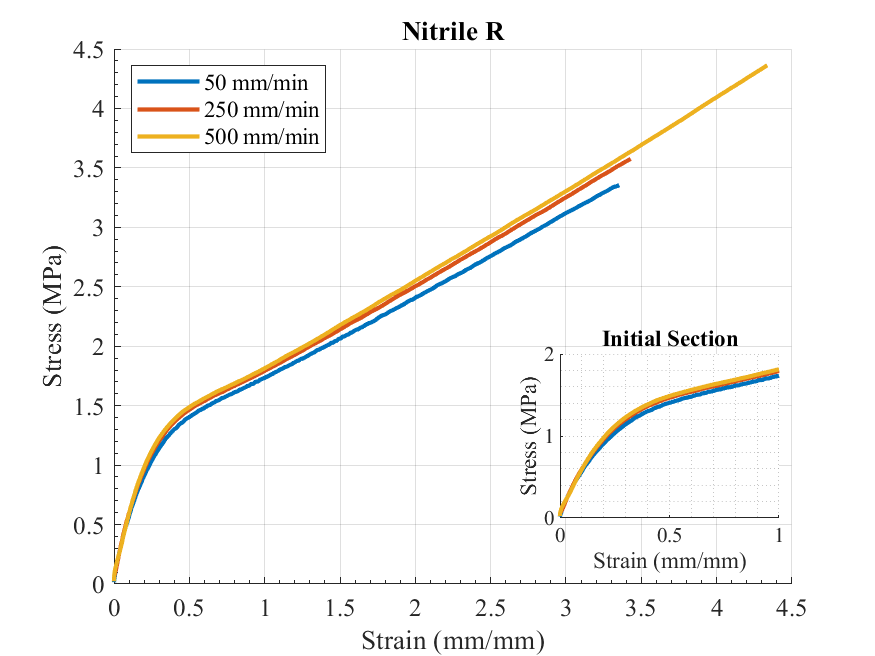
\includegraphics[width=\textwidth]{NR_StressStrain.png}
    \caption{}
    \label{sfig:NRSS}
    \end{subfigure}
    \caption{Stress-strain curves, during different strain rates, for the (a) NatPolR and (b) NR materials. On the bottom right, the initial section of the curve, where a linear behaviour was observed, is presented.}
    \label{fig:NatR-NRSS}
\end{figure}
\newpage
\begin{figure}[H]
    \vspace{-2em}
    \centering
    \begin{subfigure}[b]{0.93\textwidth}
    \centering
    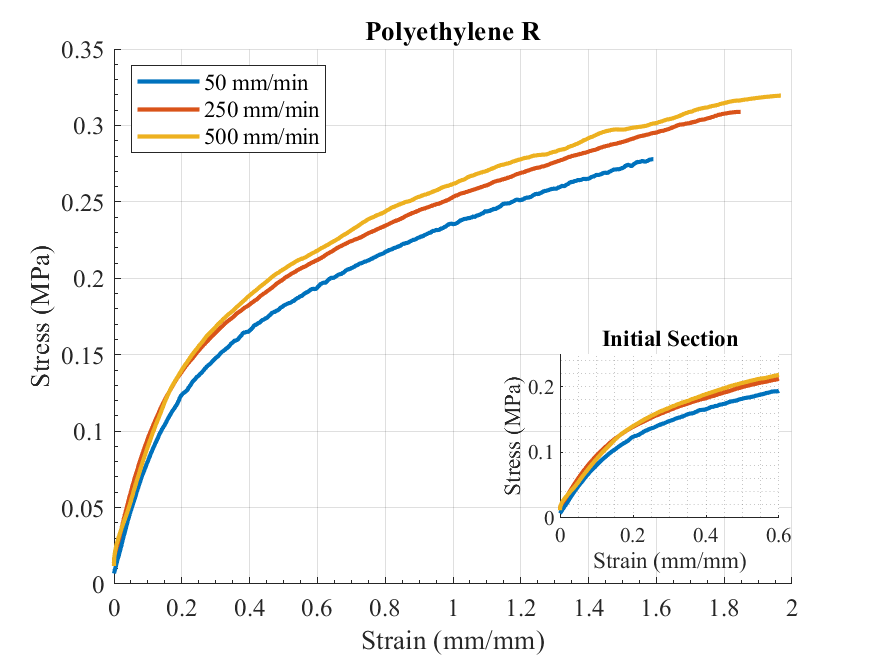
\includegraphics[width=\textwidth]{PR_StressStrain.png}
    \caption{}
    \label{fig:PRSS}
    \end{subfigure}

    \begin{subfigure}[b]{0.93\textwidth}
    \centering
    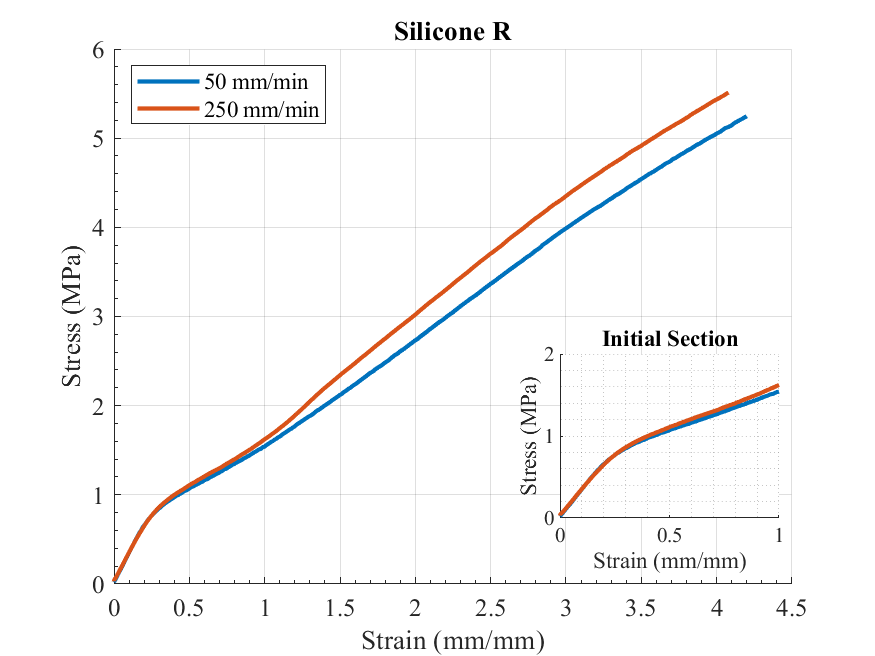
\includegraphics[width=\textwidth]{SR_StressStrain.png}
    \caption{}
    \label{fig:SRSS}
    \end{subfigure}
    \caption{Stress-strain curves, during different strain rates, for the (a) PR and (b) SR materials. On the bottom right, the initial section of the curve, where a linear behaviour was observed, is presented.}
    \label{fig:PR-SRSS}
\end{figure}
\newpage
\begin{figure}[H]
    \vspace*{-2em}
    \centering
    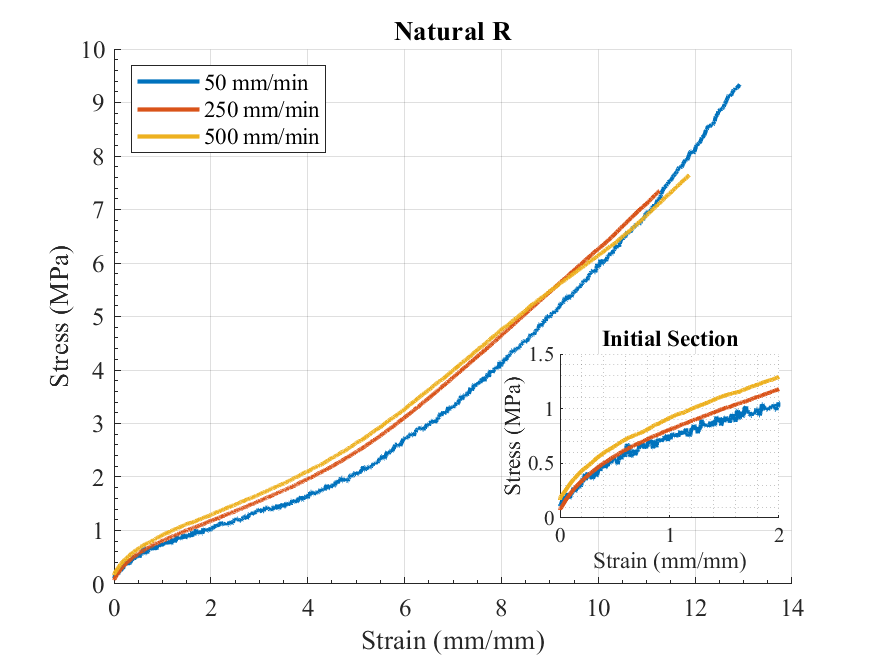
\includegraphics[width=0.93\textwidth]{Nat100R_StressStrain.png}
    \caption{Stress-strain curve, during different strain rates, for the NatR. On the bottom right, the initial section of the curve, where a linear behaviour was observed, is presented.}
    \label{fig:Nat100RSS}
\end{figure}
\vspace*{-1em}
In \Cref{fig:EPR-FRSS,fig:NatR-NRSS,fig:PR-SRSS,fig:Nat100RSS}, the velocity-dependency on the stress response of elastomers can be observed. In general, for larger strain rates, the materials exhibited a larger stress response. Moreover, a large difference in the ultimate values of the stress-strain curve of the Natural Rubber with Polyester material at 500 mm/min was observed in comparison to the other two curves (\Cref{sfig:NatRSS}). This is a side effect from the unification step in the processing of the data, which is being amplified in here due to the small number of datasets involved in the 500 mm/min tensile strength test for this material (\Cref{tbl:tensile_tests}). Also, the Natural Rubber and Fluorocarbon material showed signs of crystallization, a phenomenon described in \cite{Bauman2008} which happens when the internal molecular chains of the material are completely extended and greatly oppose to further deformation, hence the increase in stiffness just before the failure point. Moreover, most of the materials have two regions in which the proportionality between the stress and strain appears to be constant. This is inline with the expected nonlinear behaviour from elastomers previously described. The slope of these regions, i.e. the stiffness, can be approximated by linear regression. A method such as the yield offset strength can be used to separate these regions into an initial and small elastic region, and a final and large elastic region. Therefore, the offset yield strength, $\sigma_y$ and $\varepsilon_y$, is obtained and illustrated in \Cref{fig:FRoff,fig:NatRoff,fig:NRoff,fig:PRoff,fig:Nat100Roff,fig:SR-EPRoff,fig:EPR500off}.

%The correct factor to fit to figures in the same line is 0.49
\newpage
\begin{figure}[H]
    \vspace*{-2em}
    \centering
    \begin{subfigure}[b]{0.65\textwidth}
        \centering
        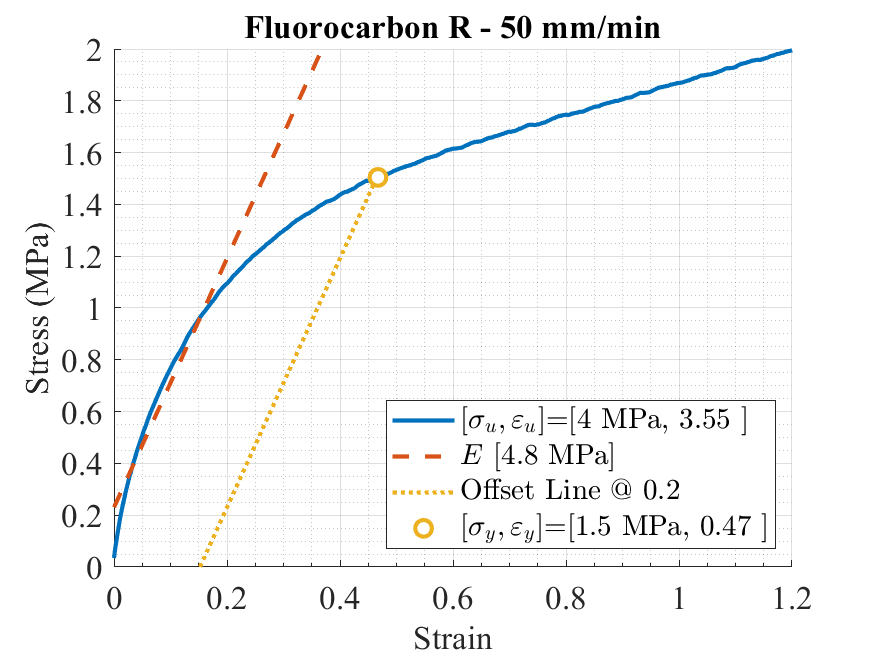
\includegraphics[width=\textwidth]{FR_disR50.png}
        \caption{}
        \label{fig:FR50}
    \end{subfigure}
    \begin{subfigure}[b]{0.65\textwidth}
        \centering
        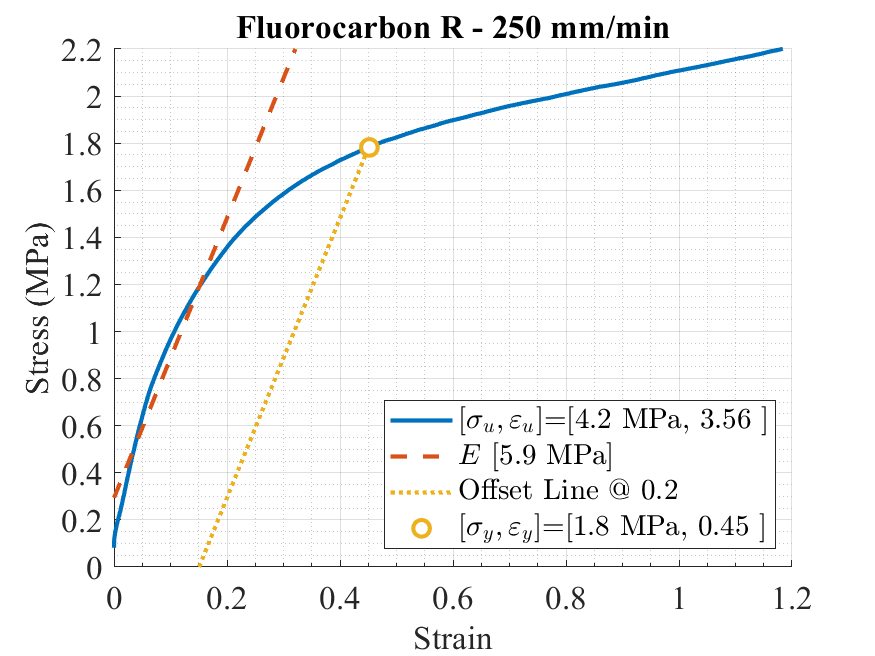
\includegraphics[width=\textwidth]{FR_disR250.png}
        \caption{}
        \label{fig:FR250}
    \end{subfigure}
    \begin{subfigure}[b]{0.65\textwidth}
        \centering
        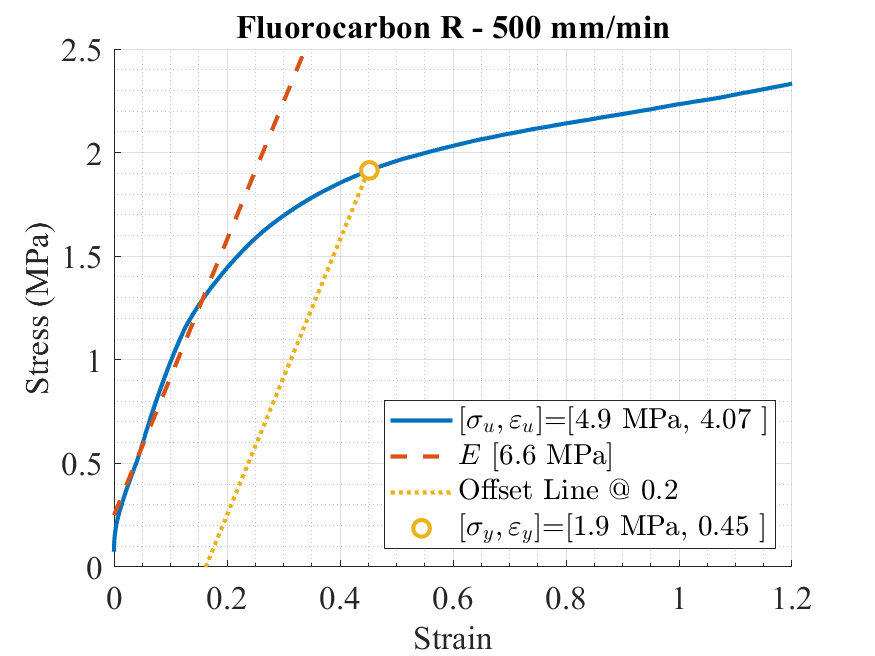
\includegraphics[width=\textwidth]{FR_disR500.png}
        \caption{}
        \label{fig:FR500}
    \end{subfigure}
    \caption{Offset Yield Strength for the FR material}
    \label{fig:FRoff}
\end{figure}
\newpage
\begin{figure}[H]
    \vspace*{-2em}
    \centering
    \begin{subfigure}[b]{0.65\textwidth}
        \centering
        \includegraphics[width=\textwidth]{NatR_disR50.png}
        \caption{}
        \label{fig:NatR50}
    \end{subfigure}
    \begin{subfigure}[b]{0.65\textwidth}
        \centering
        \includegraphics[width=\textwidth]{NatR_disR250.png}
        \caption{}
        \label{fig:NatR250}
    \end{subfigure}
    \begin{subfigure}[b]{0.65\textwidth}
        \centering
        \includegraphics[width=\textwidth]{NatR_disR500.png}
        \caption{}
        \label{fig:NatR500}
    \end{subfigure}
    \caption{Offset Yield Strength for the NatPolR material}
    \label{fig:NatRoff}
\end{figure}
\newpage
\begin{figure}[H]
    \vspace*{-2em}
    \centering
    \begin{subfigure}[b]{0.65\textwidth}
        \centering
        \includegraphics[width=\textwidth]{NR_disR50.png}
        \caption{}
        \label{fig:NR50}
    \end{subfigure}
    \begin{subfigure}[b]{0.65\textwidth}
        \centering
        \includegraphics[width=\textwidth]{NR_disR250.png}
        \caption{}
        \label{fig:NR250}
    \end{subfigure}
    \begin{subfigure}[b]{0.65\textwidth}
        \centering
        \includegraphics[width=\textwidth]{NR_disR500.png}
        \caption{}
        \label{fig:NR500}
    \end{subfigure}
    \caption{Offset Yield Strength for the NR material}
    \label{fig:NRoff}
\end{figure}
\newpage
\begin{figure}[H]
    \vspace*{-2em}
    \centering
    \begin{subfigure}[b]{0.65\textwidth}
        \centering
        \includegraphics[width=\textwidth]{PR_disR50.png}
        \caption{}
        \label{fig:PR50}
    \end{subfigure}
    \begin{subfigure}[b]{0.65\textwidth}
        \centering
        \includegraphics[width=\textwidth]{PR_disR250.png}
        \caption{}
        \label{fig:PR250}
    \end{subfigure}
    \begin{subfigure}[b]{0.65\textwidth}
        \centering
        \includegraphics[width=\textwidth]{PR_disR500.png}
        \caption{}
        \label{fig:PR500}
    \end{subfigure}
    \caption{Offset Yield Strength for the PR material}
    \label{fig:PRoff}
\end{figure}
\newpage
\begin{figure}[H]
    \vspace*{-2em}
    \centering
    \begin{subfigure}[b]{0.65\textwidth}
        \centering
        \includegraphics[width=\textwidth]{Nat100R_disR50.png}
        \caption{}
        \label{fig:Nat100R50}
    \end{subfigure}
    \begin{subfigure}[b]{0.65\textwidth}
        \centering
        \includegraphics[width=\textwidth]{Nat100R_disR250.png}
        \caption{}
        \label{fig:Nat100R250}
    \end{subfigure}
    \begin{subfigure}[b]{0.65\textwidth}
        \centering
        \includegraphics[width=\textwidth]{Nat100R_disR500.png}
        \caption{}
        \label{fig:Nat100R500}
    \end{subfigure}
    \caption{Offset Yield Strength for the NatR material}
    \label{fig:Nat100Roff}
\end{figure}
\newpage
\begin{figure}[H]
    \vspace*{-2em}
    \centering
    \begin{subfigure}[b]{0.65\textwidth}
        \centering
        \includegraphics[width=\textwidth]{SR_disR50.png}
        \caption{}
        \label{fig:SR50}
    \end{subfigure}
    \begin{subfigure}[b]{0.65\textwidth}
        \centering
        \includegraphics[width=\textwidth]{SR_disR250.png}
        \caption{}
        \label{fig:SR250}
    \end{subfigure}
    \begin{subfigure}[b]{0.65\textwidth}
        \centering
        \includegraphics[width=\textwidth]{EPR_disR50.png}
        \caption{}
        \label{fig:EPR50}
    \end{subfigure}
    \caption{Offset Yield Strength for the SR and EPR (50mm/min) material.}
    \label{fig:SR-EPRoff}
\end{figure}
\begin{figure}[H]
    \vspace*{-2em}
    \centering
    \includegraphics[width=0.65\textwidth]{EPR_disR500.png}
    \caption{Offset Yield Strength for the EPR (500mm/min) material}
    \label{fig:EPR500off}
\end{figure}

In \Cref{fig:FRoff,fig:NatRoff,fig:NRoff,fig:PRoff,fig:Nat100Roff,fig:SR-EPRoff,fig:EPR500off}, the elastic region is approximated by using the offset yield strength parameter, described previously. Also, the values for the ultimate strength, yield strength, and the elastic modulus at the elastic region, are provided. Any value below the offset yield strain can be assumed to be inside the elastic region of the material, hence the material will recover its original shape after undergoing any deformation inside this range of values. Having delimited the elastic region and its elastic modulus (now $E_{small}$), the slope of the second linear portion of the curve, i.e. the elastic modulus $E_{large}$, can be approximated. Finally, the elastic properties of the material are compiled in \Cref{tbl:elasticProp}.

In \Cref{tbl:elasticProp}, the $\sigma_{ue}$ and $\varepsilon_{ue}$ are reported as the median value from all the specimens of a specific test type. The yield values $\sigma_{y}$ and $\varepsilon_{y}$ were obtained using the offset yield strength method. The parameters $E_{small}$ and $E_{large}$ are the elastic modulus at the initial section, and middle section of the stress-strain curve. Also, $E_{small}$ is the most useful parameter for assessing the performance of a material in a real robotic application, because it describes the stiffness of a material inside the elastic region, i.e. safe working conditions. In this regards the PR material had the smallest value, whereas the NatR had the highest.

% The detailed process to calculate the offset yield strength is as follows. The first step is to apply a linear regression to the first part of the stress-strain curve. In this work, the range from 0 to 20\% strain is chosen. The slope of the fitted line represents the elastic modulus at the specified strain (20. The second step is to create a new line, starting from the specified 2\% offset strain, using the previously found elastic modulus as its slope. Finally, this line is projected up to the point in which it intersects the stress-strain curve. The stress and strain at this point represent the offset yield stress and the offset yield strain, respectively. Therefore, it is assume that beyond this point the material start undergoing plastic deformations. Similarly, it is assumed that the material is able to recover its original shape for all deformations found bellow the offset yield strain. 

\begin{table*}[htb!]
\centering
\caption{Elastic properties of the selection of soft materials. The materialas are: Polyethylene Rubber (PR), Ethylene Polypropylene Rubber (EPR), Natural Rubber with Polyester (NatPolR), Natural Rubber (NatR), Silicone Rubber (SR), Fluorocarbon Rubber (FR), and Nitrile Rubber (NR).}
\label{tbl:elasticProp}
\begin{tabular}{lccccccccc} \toprule
Materials                  & Speed & $\sigma_{ue}$ & $\varepsilon_{ue}$ & $\sigma_{u}$ & $\varepsilon_{u}$ & $\sigma_{y}$ & $\varepsilon_{y}$ & $E_{small}$ & $E_{large}$ \\
                           & mm/min   & MPa &  & MPa &  & MPa &  & MPa & MPa \\
\hline
\multirow{2}{*}{EPR}      & 50    & 8.48       & 7.56       & 7.67    & 6.74    & 1.44    & 0.54    & 3.23     & 0.99      \\
                           & 500   & 9.59       & 8.84       & 9.16    & 8.41    & 1.39    & 0.51    & 4.16     & 1.1       \\
\hline
\multirow{3}{*}{FR}      & 50    & 4.36       & 3.97       & 3.96    & 3.56    & 1.5     & 0.47    & 4.83     & 0.65      \\
                           & 250   & 4.41       & 3.93       & 4.22    & 3.57    & 1.78    & 0.45    & 5.95     & 0.58      \\
                           & 500   & 5.35       & 4.29       & 4.87    & 4.07    & 1.91    & 0.45    & 6.78     & 0.61      \\
\hline
\multirow{3}{*}{NatPolR}    & 50    & 3.57       & 1.19       & 3.08    & 0.91    & 2.12    & 0.41    & 9.97     & 2.05      \\
                           & 250   & 4.06       & 1.19       & 3.91    & 1.09    & 2.51    & 0.43    & 10.74    & 2.28      \\
                           & 500   & 4.59       & 1.64       & 4.59    & 1.64    & 2.52    & 0.48    & 8.77     & 1.9       \\
\hline
\multirow{3}{*}{NR}      & 50    & 3.55       & 3.57       & 3.36    & 3.36    & 1.41    & 0.5     & 4.29     & 0.64      \\
                           & 250   & 3.65       & 3.62       & 3.58    & 3.43    & 1.47    & 0.5     & 4.63     & 0.69      \\
                           & 500   & 4.62       & 4.61       & 4.37    & 4.34    & 1.48    & 0.5     & 4.72     & 0.72      \\
\hline
\multirow{3}{*}{PR}      & 50    & 0.3        & 1.87       & 0.28    & 1.59    & 0.18    & 0.48    & 0.58     & 0.11      \\
                           & 250   & 0.33       & 1.97       & 0.31    & 1.83    & 0.19    & 0.45    & 0.66     & 0.1       \\
                           & 500   & 0.32       & 1.97       & 0.32    & 1.97    & 0.2     & 0.49    & 0.64     & 0.1       \\
\hline
\multirow{2}{*}{SR}      & 50    & 6.03       & 5.77       & 5.26    & 4.22    & 1.1     & 0.53    & 3.26     & 1.08      \\
                           & 250   & 5.68       & 4.27       & 5.52    & 4.08    & 1.15    & 0.54    & 3.26     & 1.35      \\
\hline
\multirow{3}{*}{NatR} & 50    & 9.43       & 13.02      & 9.37    & 12.93   & 0.61    & 0.69    & 1.01     & 0.33      \\
                           & 250   & 15.88      & 12.11      & 7.38    & 11.27   & 0.69    & 0.74    & 1.11     & 0.41      \\
                           & 500   & 11.93      & 12.26      & 6.61    & 11.22   & 0.73    & 0.71    & 1.19     & 0.43     \\
\bottomrule
\end{tabular}
\end{table*}


\subsection{Stress Relaxation Test}

The stress relaxation test allows the extraction of the viscoelastic properties of the materials, i.e. the time-dependent properties. In this test, a predefined and constant elongation, also called initial strain $\varepsilon_o$ is applied to the material specimen. The material is held in place for the whole duration of the test and the stress response is recorded. The material will relax over time, i.e. the stress response will decrease. Similarly as for the tensile strength test, different combinations of test duration and initial strain values were chosen for the tests. Also, a varying number of specimens were included in each test. Some of these combinations were based on similar characterization processes available in the literature in where the duration time was no longer than 200 minutes \cite{case2015soft,delin1995volume}. Nonetheless, a second test is proposed with a shorter duration. The diverse parameters used in the tests are aimed to create a richer dataset. As a recommendation, the value for the applied $\varepsilon_o$ must fall beyond the elastic region of the material to avoid plastic deformation, i.e. irreparable damage. However, for highly elastic materials, such as elastomers, large values of $\varepsilon_o$ are used in the literature. Also, the material must be elongated from zero strain to the value of $\varepsilon_o$ as fast as possible. Therefore, the strain rate chosen for this test was  500 mm/min. With this in mind, the first test was performed using relatively large values of $\varepsilon_o$ which were beyond the elastic region of the materials, identified in \Cref{sss:elasticProperties}. For this case, the test duration was the longest, of 180 minutes. A second test was performed using $\varepsilon_o$ values inside the elastic region of the materials and with a shorter duration of 15 minutes. The parameters for the performed tests are compiled in \Cref{tbl:stressRelParameters}.

\begin{table*}[htbp!]
\centering
\caption{Parameters and number of collected datasets for the stress relaxation tests.}
\label{tbl:stressRelParameters}
\begin{tabular}{llccccccc} \toprule
Test & Parameters & EPR & FR & NatPolR & NR & PR & SR & NatR \\
\hline
\multirow{4}{*}{1}  & $\Delta L_o$ (mm)      & 5 & 5 & 7 & 6 & 3 & 6 & 40 \\
                    & $\varepsilon_o$	   & 0.15 & 0.15 & 0.21 & 0.18 & 0.09 & 0.18 & 1.21 \\
                    & Duration (minutes)    & 15 & 15 & 15 & 15 & 15 & 15 & 15 \\
                    & Datasets              & 5 & 5 & 5 & 5 & 5 & 5 & 2 \\
\hline 
\multirow{4}{*}{2}  & $\Delta L_o$ (mm)      & 20 & 10 & 6 & 5 & 4 & 15 & - \\
                    & $\varepsilon_o$	   & 0.61 & 0.3 & 0.18 & 0.15 & 0.12 & 0.45 & - \\
                    & Duration (minutes)    & 180 & 180 & 180 & 180 & 180 & 180 & 180 \\
                    & Datasets              & 1 & 1 & 1 & 1 & 1 & 1 & - \\
\bottomrule
\end{tabular}
\end{table*}

Similar to the tensile strength tests, the collected data was processed prior to the extraction of the relevant parameters. The data of interest is the one found after the machine has reached the predefined $\varepsilon_o$ value. In here, several smoothing algorithms such as, moving average, Gaussian-weighted moving average, and the Savitzky-Golay algorithm, were analyzed. During testing of these algorithms, a direct relationship between the decrease in the value of the initial stress $\sigma_o$, and the selected window size, was observed. The selected window size was based on the sampling frequency and the duration of the test. The Savitzky-Golay algorithm has the least impact on the initial stress $\sigma_o$ in relation to the achieved smoothing, hence it performed better than the other two algorithms.

\subsubsection{Stress Relaxation Properties}

The stress relaxation test is useful for approximating the time relaxation constants of the materials. Commonly, viscoelastic materials have more than one relaxation constant. This is caused by the many number of internal molecular chains which relax at different rates. The stress relaxation curve of viscoelastic materials exhibit a decaying exponential stress relaxation curve. This known mathematical function, in combination with the LVMs, can be used to approximate the time relaxation constants of the material. The LVMs have the flexibility to get as complex as required by adding extra elements to the model. The latter means that the number of relaxation constants that can be extracted from the stress relaxation curve is directly proportional to the number of exponential functions contained in the LVM. This is described in detail in \Cref{sec:ChapterModellingLVM}. The stress at the starting and ending points of the test,  $\sigma_o$ and $\sigma_{end}$, respectively, are the minimum required parameters to approximate one relaxation constant of the material using a LVM. Another parameter of interest is the achieved stress relaxation, which is defined as follows:

\begin{equation}
	S.R. = 100\left( \frac{\sigma_o - \sigma_{end}}{\sigma_o}\right) 
\end{equation}

The parameters extracted from the stress relaxation test are compiled in \Cref{tbl:stressRelProperties}. The obtained stress relaxation curves of all the materials are illustrated in \Cref{fig:AllSRel,fig:PRSRel}. The values of $\sigma_o$ and $\sigma_{end}$ are obtained by finding the median value of all tests included in each scenario, using the collected raw data. The values of the $S.R.$ are very similar in both tests, in terms of the duration of the test and the chosen value for $\varepsilon_o$.  This means most of the S.R. happens very early into the test, and that only one relaxation time constant is required to model the stress relaxation of these materials.

\begin{table*}[htb!]
\centering
\caption{Stress relaxation properties for the selection of soft materials.}
\label{tbl:stressRelProperties}
\begin{tabular}{llccccccc} \toprule
Test & Properties & EPR & FR & NatPolR & NR & PR & SR & NatR \\
\hline
\multirow{3}{*}{1}  & $\sigma_o$ (MPa)   & 0.61      & 0.84      & 1.22      & 0.77      & 0.06      & 0.61      & 2.15 \\
                & $\sigma_{end}$ (MPa)    & 0.42      & 0.27      & 0.80      & 0.55      & 0.02      & 0.43      & 1.82 \\
                & $S.R. (\%)$    &  32     & 67      & 35      & 29      & 63      & 31      & 15 \\
                     
\hline 
\multirow{3}{*}{2}  & $\sigma_o$ (MPa)     & 1.28      & 1.13      & 1.18      & 0.72      & 0.07      & 1.11  &         \\
                & $\sigma_{end}$ (MPa)     & 0.89      & 0.41      & 0.76      & 0.55      & 0.03      & 0.80  &          \\
                & $S.R. (\%)$     & 31      & 63      & 36      & 24      & 51      & 28  &          \\
\bottomrule
\end{tabular}
\end{table*}


\begin{figure}[H]
    \centering
        \begin{subfigure}[b]{0.93\textwidth}
        \centering
        \includegraphics[width=0.9\textwidth]{All180SRel.png}
        \caption{Caption}
        \label{sfig:ALL180SRel}
    \end{subfigure}
    \begin{subfigure}[b]{0.93\textwidth}
        \centering
        \includegraphics[width=0.9\textwidth]{All15SRel.png}
        \caption{Caption}
        \label{sfig:centering}
    \end{subfigure}
    \caption{Stress Relaxation curves for (a) 180 minutes and (b) 15 minutes, of the EPR, FR, NatPolR, NR and SR materials. Different values of $\varepsilon_o$ were investigated.}
    \label{fig:AllSRel}
\end{figure}

\newpage
\begin{figure}[H]
    \centering
        \begin{subfigure}[b]{0.93\textwidth}
        \centering
        \includegraphics[width=0.9\textwidth]{PR180SRel.png}
        \caption{Caption}
        \label{sfig:PR180SRel}
    \end{subfigure}
    \begin{subfigure}[b]{0.93\textwidth}
        \centering
        \includegraphics[width=0.9\textwidth]{PR15SRel.png}
        \caption{Caption}
        \label{sfig:PR15SRel}
    \end{subfigure}
    \caption{Stress Relaxation curves for (a) 180 minutes and (b) 15 minutes, of the PR, and NatR materials. Different values of $\varepsilon_o$ were investigated.}
    \label{fig:PRSRel}
\end{figure}


%In this paragraph I could mention that depending on the linearity of the stress relaxation curve plotted in logarithmic scale, one can assume how many relaxation times are present. This part could be more suitable on the modelling chapter.

%More information on the stress relaxation modulus can be found in the Book Engineering Viscoelasticity. Although, the relevance of bringing this information in here is not clear.



\section{Summary}

In this chapter, the characterization process of the viscoelastic mechanical properties of a selection of seven different TPEs was presented. For this, the mechanical tests of tensile strength and stress relaxation was performed. In the tensile strength test, the materials were elongated until failure using up to three different strain, or elongation, rates. The latter will allow the modelling of the velocity-dependent stress response of the materials. The processing algorithm used to condition the collected data was also described in detail. The smoothing algorithm chosen for both mechanical tests was the Savitsky-Golay algorithm. In the case for the Natural Rubber material, where two batches were acquired, the thickness from one batch to the other varied significantly. Nevertheless, the mechanical behaviour of the material was captured accurately in the stress-strain curves. This suggests a linear proportionality between the thickness of the material and the increment on the response of the material. The elastic region of the materials was difficult to be identified directly due to their nonlinear stress-strain curve. Therefore, the elastic region was approximated using the offset yield strength parameter. This region is very important to delimit the working conditions of the soft materials in a real robotic application. Finally, the ultimate values of strain and stress, the elastic region location, the elastic modulus in two distinctive regions of the curve, and the offset yield strength parameters, were reported. The $E_{small}$ is the most useful parameter for assessing the performance of a material in a real robotic application, because it describes the stiffness of a material inside the elastic region, i.e. safe working conditions, in contrast to the ultimate strength values. In this regard the PR material had the smallest value, whereas the NatR had the highest.

The performed stress relaxation tests can be divided into two sets. One with a low deformation, and low duration. The other, with large deformation, large duration. Regarding this, the achieved stress relaxation of the materials was very similar for both cases. Knowing the resemblance of the stress relaxation curve with an exponential decaying function, the latter finding could suggest that only one relaxation time constant is responsible for the majority of the $S.R.$ achieved.  This hypothesis will be explored in the modelling stage. 

%Finish this chapter by: Checking Captions. Additionally, make each chapter start on an even page. Plots need to be redone
\newpage\null\thispagestyle{plain}\newpage
\chapter{Soft Materials Modelling: Linear Viscoelastic Models} \label{sec:ChapterModellingLVM}

%NOTE: This paper is a good literature for the next chapter about modelling, "Soft Material Characterization for Robotic Applications". In here there is a section about the variability of the materials properties from one batch to the other. However there is a consistency from specimens from the same batch

\section{Introduction}

In this chapter, two modelling tools, based on mathematical models, for the prediction of the viscoelastic properties of seven soft materials are developed. These models are the PL-SLS model and the PL-Wiechert model. The work carried out in this chapter is inspired on the piecewise linearisation (PL) method described by Austin et al. \cite{austin2015control}. The PL method has been proven successful in enabling the Standard Linear Solid (SLS) model to account for the strain-dependent stress response of soft materials. The model developed in Austin et al. work is called the Standard Linear Solid model with Strain-Dependent Stiffness (Std. Lin. SDS). The capabilities of the Std. Lin. SDS of accounting for velocity-dependent stress responses have not been assessed in the literature. This is investigated in this chapter. 

The PL method implemented in this work is improved to maximize the prediction performance of the models. Due to this, the developed models in here differ from the ones available in the literature and represent a direct improvement to current modelling approaches. Two LVMs are studied in here, the SLS model and the Wiechert model. The PL method is applied to both, yielding the PL-SLS and the PL-Wiechert models. The Wiechert model is of interest due to its better capabilities of accounting for velocity-dependent stress responses, in comparison to the simpler SLS model. These additional capabilities of the Wiechert model translates into additional computational and mathematical complexity. Nonetheless, the PL method is capable of reducing this complexity.

In contrast with the fitting process described in the literature \cite{austin2015control}, the stress relaxation test is used to extract the relevant parameters for the SLS and Wiechert models. Subsequently, the PL method is applied to both models, allowing them to account for strain-dependent stress responses. The performance of both models is assessed using the stress-strain curves of the characterized soft materials: ethylene polypropylene rubber (EPR \cite{EPRubber2019}), fluorocarbon rubber (FR \cite{FRubber2019}), nitrile rubber (NR \cite{NRubber2019}), natural rubber with polyester (NatPolR \cite{NatPolRubber2019}), polyethylene  rubber  (PR \cite{PRubber2019}), silicone  rubber  (SR \cite{SRubber2019}), and natural rubber (NatR \cite{NatRubber2019}).

Three mains analyses are performed. Firstly, the relationship between the PL method prediction accuracy and required complexity is assessed. A tolerance criteria is proposed in here, which establishes a proportional relationship between the complexity of the soft material stress-strain curve, and the required complexity of the PL method. Secondly, the maximum prediction accuracy of both models is assessed. The results indicate that both models can accurately predict the stress-strain curve of the soft materials under a single strain rate. Thirdly, the capabilities of both models to account for the velocity-dependent stress response of the materials are investigated. The results indicate the superiority of the PL-SLS model and the PL-Wiechert model in comparison to the Std. Lin. SDS model documented in the literature. The models developed in here achieved normalized root mean square values of 5\% in comparison to the 13.6\% achieved by the Std. Lin. SDS model. In general, the PL-Wiechert model performs better for soft materials with moderate to high viscous properties, whereas the PL-SLS model performed better for soft materials with high elastic properties. In conclusion, the improved implementation of the PL method resulted in an improved modelling tool for the prediction of the nonlinear, strain-dependent, and time-dependent stress response of soft materials.

\section{The Linear Viscoelastic Models}

Thermoplastic elastomers have nonlinear and viscoelastic mechanical properties which cannot be easily described by mathematical models. The latter represents an important challenge for current soft robotic developments. However, the benefits of using soft materials are many: energy storing, passive compliance and safe human-robot interaction. This has motivated their implementation in robotic applications, as well as the development of robust modelling tools capable of describing their viscoelastic properties \cite{lee2017soft}.

The natural property of the human skeletal muscle system of storing and releasing energy, has motivated the inclusion of elasticity in robotic applications. Series-elastic actuators (SEAs) are the most commonly used technology. The addition of an elastic element between the actuator and the load greatly simplifies the controller design. The deformation of the elastic element can provide an indirect measurement of the applied force to the load, essentially transforming a force-control problem into a displacement-control problem \cite{agarwal2017series}. 

Traditional SEAs use metallic springs, considered as purely elastic. However, the human skeletal muscle system exhibits viscoelastic behaviour. In the literature, attempts of adding viscoelasticity to SEAs by using soft materials instead of metallic springs, are documented. In fact, viscoelasticity has the potential to address many of the limitations found in series-elastic actuators, such as: low torque resolution and low bandwidth \cite{martins2015polyurethane,tagliamonte2014rendering,schepelmann2014compact}. 

The mechanical behaviour of a rigid element (metallic spring) can be accurately described by known mathematical models. This is not the case for soft materials which have nonlinear and viscoelastic properties. The benefits of adding viscoelasticity to SEAs can only be fully exploited by developing a  reliable modelling tool. Substantial research has been done on this. However, the most accurate models are mathematically complex and computationally expensive \cite{xu2014mathematical,ciniello2017identifying,lu2017constitutive}. Nonetheless, even these complex models cannot account for all the different factors which modify the materials properties, such as the manufacturing process and internal weakening of the material after being loaded for the first time \cite{case2015soft}. The latter highlights the difficulty of developing mathematical models which account for both microscopic and macroscopic aspects of the materials. This has motivated researchers to implement alternative methods for characterizing a material, such as Finite Element Analysis (FEA).

In robotic applications, where the controller can compensate inefficiencies in the system, a simple and fairly accurate modelling tool is preferred over a very accurate and highly complex one. For this reason, a known set of mathematical models, the Linear Viscoelastic Models (LVMs) are commonly used for the prediction of viscoelasticity in soft materials. In contrast to the mechanical model for Hooke's Law, which is based on a single spring, the LVMs are based on two fundamental mechanical components, a spring and a dashpot, which can be arranged in different configurations and quantities. This is illustrated in \Cref{fig:LinearViscoelasticModels}, where the parameters $k$ and $\eta$ represent the spring stiffness and the dashpot viscous constant, respectively.

\begin{figure}[hbt!]
	\centering
    \includegraphics[width=0.6\textwidth]{HookeViscoelasticModels.PNG}
    \caption[Hooke's Law and linear viscoelastic models: (a) Hooke's Law (b) Kelvin-Voigt, (c) Maxwell, (d) Standard Linear Solid, and (e) Burger. The parameters $k$ and $\eta$ represent the spring stiffness and the dashpot viscous constant, respectively.]{Hooke's Law and linear viscoelastic models: (a) Hooke's Law (b) Kelvin-Voigt, (c) Maxwell, (d) Standard Linear Solid, and (e) Burger. The parameters $k$ and $\eta$ represent the spring stiffness and the dashpot viscous constant, respectively \cite{austin2015control}. }
    \label{fig:LinearViscoelasticModels}
\end{figure}

In line with the mentioned approach of relying on the controller to compensate the limitations of simple models, the work performed by Austin et al. modifies the viscoelastic Standard Linear Solid (SLS) model by implementing a piecewise linearisation (PL) method \cite{austin2015control}. The authors chose the SLS model instead of the more complete, hence more complex, Burger model to keep the modelling process as simple as possible. The implementation of the PL method allowed the SLS model to account for the nonlinear properties of the material stress response in proportion to the applied strain. Due to this, the developed model is called the Standard Linear Solid model with Strain-Dependent Stiffness (Std. Lin. SDS). Unfortunately, the developed model is still incapable of accounting for the material hysteresis. Due to hardware limitations, the velocity-dependent stiffness effects are not validated. Nonetheless, experimental tests validated the changes on the material stiffness depending on the velocity of the applied deformation.

The PL method has proven to be a successful way to improve the prediction capabilities of traditional LVMs. Although it still has some limitations. The latter is addressed in this chapter by implementing the PL method in a more complex member of the LVMs, the Wiechert model.

\section{The Piecewise linearisation Method} \label{sec:wiechert}

The SLS model is frequently used when modelling viscoelastic materials, mainly due to its mathematical simplicity and its capability of accounting for the creep and stress relaxation phenomena of the materials (time-dependent properties). The SLS model can be viewed as a Maxwell model (also known as Maxwell branch) with an extra spring connected in parallel. The simplicity of the SLS model is also its main limitation. 
Viscoelastic materials are known to have more than one relaxation time constant, i.e. more than one Maxwell branch. In the family of LVMs, the relaxation time constant depends on the viscous elements, i.e. dashpots. The Wiechert model, which is essentially a SLS model with $j$ Maxwell branches, is able to account for $j$ relaxation time constants (\Cref{fig:wiechert}). The time-dependent behaviour of any viscoelastic material can be fully described by this model, given enough numbers of elements. However, the complexity of the model increases in proportion to the number of extra branches. Mathematically, each extra branch increases the derivative order of the model since more equations are required to account for the extra variables \cite{tirella2014strain,roylance2001engineering}.

\begin{figure}[hbt!]
	\centering
    \includegraphics[width=0.3\textwidth]{WiechertModel.png}
    \caption{Wiechert Model. The components $k_1$, $\eta_1$, and the equilibrium spring $k_e$, together represents the SLS model. The components $k_j$, and $\eta_j$ represents the Maxwell Branch. The Wiechert model can contain as many branches as required, this is symbolised by the subscript $j$. }
    \label{fig:wiechert}
\end{figure}

As previously described in \Cref{sec:mechprop}, in addition to time-dependent and history-dependent properties, elastomers also have a nonlinear stress response. This can be partially described by the LVMs. The relaxation time constant of the dashpots in these models describes the nonlinear and time-dependent stress response of the material. Nonetheless, LVMs cannot account for the strain-dependent response of materials. The latter can be addressed by the PL method as described in \cite{austin2015control}.

The spring in parallel with the other elements, in both the SLS model and the Wiechert model, is known as the equilibrium spring, and its stiffness $k_e$, is assumed constant. In reality, the stiffness $k_e$ of most elastomers is strain-dependent. Early attempts of modelling a strain-dependent stress response in viscoelastic materials are described by Schepelmann et al. in \cite{schepelmann2014compact}, where the stress-strain curve of a nonlinear rubber spring is approximated with an exponential model. In subsequent works, Austin et al. describe a piecewise linear regression fitted to the stress-strain curve of a material, in combination with the SLS model \cite{austin2015control}. 

The slope of the stress-strain curve represents the material's Young Modulus which is proportional to the material stiffness. During a tensile strength test the material is deformed at a constant rate, i.e. $\dot{\varepsilon}$ is constant. The stress response of a viscous element is proportional to the strain rate $\dot{\varepsilon}$. Therefore, it can be safely assumed that the observed nonlinear stress response on the stress-strain curve is solely caused by changes in the equilibrium spring stiffness $k_e$.

Using the PL method, the nonlinear behaviour of the equilibrium spring is approximated by considering it as several springs in parallel which ``engage'' in sequence as the material strain increases. This is modelled by a summation of Heaviside functions centred in the desired strain in which each of the mentioned springs ``engage'' and contributes to the total stress response of the material. In other words, the stress-strain curve of the material is segmented in several sections which relates a single stiffness to a range of strains (\Cref{fig:PLmethod}).

\begin{figure}[htb!]
	\centering
    \includegraphics[width=0.6\textwidth]{PLmethod.png}
    \caption[(a) Standard Linearized Solid model with Strain-Dependent Stiffness. (b) Piecewise linearisation method applied to the slope of the material load-displacement curve. This is analogous to many parallel springs which contribute to the material response depending on the material strain.]{(a) Standard Linearized Solid model with Strain-Dependent Stiffness. (b) Piecewise linearisation method applied to the slope of the material load-displacement curve. This is analogous to many parallel springs which contribute to the material response depending on the material strain \cite{austin2015control}.}
    \label{fig:PLmethod}
\end{figure}

\section{Model fitting} \label{sec:Modelfit}

The mathematical expression for the SLS model and the Wiechert model can be simplified when considering a constant strain input (stress relaxation test). This simplification allows these models to be fitted into the stress relaxation curve and to approximate the parameters of interest, $k$ and $\eta$ \cite{roylance2001engineering}. The mathematical expression for the Wiechert model under a constant strain input is given by:

\begin{equation}
\label{eq1}
\sigma (t) = \left( k_e +  \sum_{j} k_j e^{-t/\tau_j} \right)  \varepsilon_o
\end{equation}

\noindent where $\sigma$ is the stress at a given time, $k_e$ is the equilibrium spring stiffness and $\varepsilon_o$ is the initial strain. For the summation, $\tau_j=\eta_j/k_j$ is the relaxation time constant, $k_j$ and $\eta_j$ are the spring stiffness and viscous constant of the elements in the $j^{th}$ Maxwell branch, respectively. For the specific case when $j = 1$, the resulting equation describes the SLS model under a constant strain input, which is as follows:

\begin{equation}
\label{eq11}
\sigma(t) = \left( k_e +  k_1 e^{-t/\tau} \right)  \varepsilon_o
\end{equation}


In \Cref{eq11}, the three main parameters of the SLS model, i.e. the equilibrium spring stiffness $k_e$, the dashpot viscous constant $\eta = \tau k_1$, and the spring stiffness in the Maxwell branch $k_1$, can be obtained from the stress relaxation curve by analysing three significant points: $t=0$, $t=\tau$, and $t=\infty$ (\Cref{fig:stressTimeCurve}). Due to the decaying exponential nature of this curve, the time constant $\tau$ can be related to the point in time $t$ where the stress has decayed to approximately 36.8\% of its initial value $\sigma_o$. The longer the duration of the test, the better the approximation of $k_e$.

\begin{figure}[htb!]
	\centering
    \includegraphics[width=0.5\textwidth]{StressTimeCurve.png}
    \caption{SLS model fitted to a typical stress relaxation curve of a viscoelastic material. The parameters $k_e$, $k_1$ and $\eta$ can be obtained by analysing three points in the curve: $t=0$, $t=\tau$, and $t=\infty$. The variable $\tau$ is the time constant of the exponential decaying curve.}
    \label{fig:stressTimeCurve}
\end{figure}

The process to extract the parameters of the Wiechert model is more complicated due to its extra Maxwell branches, i.e. there are more than three points in time to be analysed. These points can be selected using a collocation technique \cite{roylance2001engineering,machiraju2006viscoelastic}. In the reviewed literature, the points of interest are linearly scattered throughout the whole duration of the stress relaxation curve. Nevertheless, the decaying exponential term in \Cref{eq1} is better approximated by selecting the points of interest using a logarithmic scale. This is possible with the MATLAB function \texttt{logspace} which spreads evenly the desired number of points between the allowable decades. 
This is best described in the following example. A Wiechert model with six branches, $j=6$, is to be fitted into a stress relaxation curve with four decades of duration ($t=10^4$ seconds). In total, it would be required seven points in time, one for each branch and one for $t=0$. These points are spread as evenly as possible, using the total duration of the test, by the function \texttt{logspace}. 

Similar to the process illustrated in \Cref{fig:stressTimeCurve}, each point in time represents a time constant $\tau_j$ for which there is a known stress $\sigma_j$ from the experimental data. This can be rearranged into an system of $j$ equations with $k_j$ as the unknown variable as follows \cite{machiraju2006viscoelastic}: 

\begin{align}
\begin{split}
k_e + k_1e^{-\tau_1/\tau_1} 	 +k_2e^{-\tau_1/\tau_2}	\dots 	 +k_je^{-\tau_1/\tau_j} 	&= \frac{\sigma(\tau_1)}{\varepsilon_0 }
\\
k_e + k_1e^{-\tau_2/\tau_1} 	 +k_2e^{-\tau_2/\tau_2}	\dots 	 +k_je^{-\tau_2/\tau_j} 	&= \frac{\sigma(\tau_2)}{\varepsilon_0 }
\\
 & \vdots
\\
k_e + k_1e^{-\tau_j/\tau_1} 	 +k_2e^{-\tau_j/\tau_2}	\dots 	 +k_je^{-\tau_j/\tau_j} 	&= \frac{\sigma(\tau_j)}{\varepsilon_0 }
\end{split}
\label{eq12}
\end{align}

Prior to this step, $k_e$ can be obtained using the equation for $\sigma(\infty)=\varepsilon_o k_e$, as illustrated in \Cref{fig:stressTimeCurve}. Subsequently, the Wiechert model in \Cref{eq1} can be completely described by solving the system of equations described in \Cref{eq12}. Finally, after obtaining all the $k_j$, the value of $k_1$ is corrected by analysing the point in time $t=0$, as described in \cite{roylance2001engineering}. 

The previous process allows the Wiechert model equation to be fitted into the stress relaxation curve for a defined number of branches $j$. However, to obtain the optimal number of branches for each material, an iterative algorithm to find the smallest root mean square error (RMSE) between the Wiechert model response and the experimental data after testing a different number of branches in the range of $j=[1,10]$ is implemented. The obtained optimal number of branches for each material varies between the range $j=[5,8]$. A higher number of branches have a meaningless improvement on the RMSE. Furthermore, beyond the number of branches $j=20$ the Wiechert model response shows an oscillatory behaviour, hence a higher RMSE. 

Having obtained the parameters of interest for the SLS and the Wiechert model, their stress response under a constant strain is compared against the experimental data in \Cref{fig:StressRelFit}. In this figure the superior accuracy delivered by the extra Maxwell branches in the Wiechert model in comparison to the simpler SLS model is observed. 

\begin{figure}[htb!]
	\centering
	\includegraphics[width=0.8\textwidth]{SRelFit.png}
	\caption{Obtained fit from the Standard Linear Solid (SLS) and Wiechert model of the stress relaxation curve of the Silicone Rubber material. The obtained optimal number of branches of the Wiechert model fit is $j=8$.}
	\label{fig:StressRelFit}
\end{figure}

As previously mentioned, \Cref{eq1} is a simplification helpful to approximate the parameters of both models, but it is only applicable when the strain input is constant. The mathematical expression for the Wiechert model which describes the stress response under an unknown strain input, also called the constitutive equation, in the Laplace domain, is as follows \cite{roylance2001engineering}:

\begin{equation}
\label{eq13}
\bar{\sigma} = \bar{\sigma_e} + \sum_j \bar{\sigma_j} = \left\{ k_e + \sum_j \frac{k_j s}{ \left(s + \frac{1}{\tau_j} \right) } \right\} \bar{\varepsilon}
\end{equation}

\noindent where $\bar{\sigma}$ is the total stress,$ \bar{\sigma_e}$ is the stress of the equilibrium spring, $\bar{\sigma_j}$ is the stress of the Maxwell branches, and $\bar{\varepsilon}$ is the strain function. All these variables are in the Laplace domain.  Similarly, the constitutive equation for the SLS model, i.e. $j=1$, in its time domain, is as follows:

\begin{equation}
\label{eq3}
\dot{\sigma} + \frac{\sigma}{\tau_1} =  (k_e + k_1)\dot{\varepsilon} + \frac{k_e\varepsilon}{\tau_1}
\end{equation}

\noindent where $\varepsilon$, $\dot{\varepsilon}$, and $\dot{\sigma}$ are the strain, the strain rate and the stress rate, respectively (for the detailed procedure refer to \cite{roylance2001engineering}). Notice that the previous procedure will yield into a higher derivative order equation when applied to the Wiechert model due to its extra branches. A higher number of branches will increase the model accuracy at the cost of increasing its mathematical complexity. The constitutive equation of a Wiechert model with $j$ branches would result in a $j^{th}$ order differential equation similar to \Cref{eq3}. The aim of this chapter is to apply the PL method to the Wiechert model and evaluate its performance. Therefore, dealing with differential equations is out of the scope. Nonetheless, the Wiechert model can be evaluated by transforming it into a finite-differences equation yielding the following equation \cite{roylance2001engineering}:

\begin{equation}
    \label{eq4}
    \sigma^t = k_e\varepsilon^t + \sum_j \frac{k_j(\varepsilon^t - \varepsilon^{t-1}) + \sigma_j^{t-1}}{ \left( 1+\dfrac{\Delta t}{\tau_j} \right) }
\end{equation}

\noindent where the superscript $t-1$ and $t$ refers to values before and after a small time step $\Delta t$ have passed. Once again, making $j=1$ in \Cref{eq4} yields the finite difference version of the SLS model. 

The next step of the fitting process is focused on the tensile strength test. In this test, the strain rate is constant, hence the resulting stress for both models is dependent on both the equilibrium spring and the Maxwell branches. At this stage of the model fitting process, the parameters of the Maxwell branches in both models are known and their stress response can be calculated. The stress response in the equilibrium spring $k_e$ can be isolated by subtracting the stress response of the Maxwell branches to the stress measured in the tensile strength test. 

After isolating the stress response of $k_e$, the final step in the fitting process is to implement the PL method to both models and compare their response against the experimental data. Firstly, the stress-strain curve from the tensile strength test is divided into $n$ segments. As previously explained, $k_e$ is considered as a group of parallel springs which ``engage'' as the strain increases. This means, each subsequent stiffness is a combination of the ones found in previous segments of the stress-strain curve (\Cref{fig:PLmethod}).  Lastly, a linear regression is applied to the stress-strain curve for the desired $n$ strain segments to find the slope of the curve. This slope represents the stiffness of the equilibrium spring in each segment. By combining the $n$ obtained stiffness, the stress response of the strain-dependent stiffness $k_i^*$ is defined as follows:

\begin{equation}
\label{eq5}
\sigma^{*^t} = \sum_i^n k_i^* H_{\varepsilon - \varepsilon_i}(\varepsilon^t - \varepsilon_i)
%\sigma^* = \sum_i^n k_i^* H_{\varepsilon - \varepsilon_i}(\varepsilon - \varepsilon_i)
\end{equation}

\noindent where $n$ is the desired number of strain intervals to fit, $\varepsilon_i$ represents the strain value at which the $i^{th}$ spring starts contributing to the stress response, the $H_{\varepsilon - \varepsilon_i}$ is the Heaviside or unitary step function centered at $\varepsilon_i$, i.e. the function output goes from 0 to 1 when $\varepsilon - \varepsilon_i = 0$. By substituting \Cref{eq5} into \Cref{eq3}, the Standard Linear Solid model with Strain-Dependent Stiffness is obtained \cite{austin2015control}.

The LVMs describe a nonlinear relationship between the applied strain and the resulting stress in a material. However, they only account for a linear stress response of the equilibrium spring. In reality, the relocation of internal molecular chains causes viscoelastic materials to exhibit a nonlinear and strain-dependent stress response. This can be solved by applying the PL method to \Cref{eq4}. The equilibrium spring stiffness $k_e$ is replaced by the strain-dependent stiffness $k_i^*$, yielding the linearized Wiechert model (PL-Wiechert) in \Cref{eq6}. Subsequently, the Std. Lin. SDS model, found in \cite{austin2015control}, is transformed into a finite difference equation, yielding the PL-SLS model described in \Cref{eq7}.

\begin{equation}
\label{eq6}
\sigma^t = \sigma^*{^t} + \sum_j \frac{k_j (\varepsilon^t-\varepsilon^{t-1}) + \sigma_j^{t-1}}{\left( 1 + \dfrac{\Delta t}{\tau_j}\right) }
\end{equation}

\begin{equation}
\label{eq7}
\sigma^t = \sigma^*{^t} + \frac{k_1(\varepsilon^t - \varepsilon^{t-1}) + \sigma_m^{t-1}}{ \left( 1+\dfrac{\Delta t}{\tau_1} \right) }
%\sigma^ t = \frac{1}{\left( 1+\dfrac{\Delta t} {\tau} \right) } \left[  \frac{\Delta t}{\tau} \sigma^* + (\sigma^* + k_1) (\epsilon^t-\epsilon^{t-1}) + \sigma^{t-1} \right]  
\end{equation}

The linearized SLS model \Cref{eq7} is labelled as the Piecewise Linearized SLS (PL-SLS) model, differentiating it from the Std. Lin. SDS model due to the many optimizations performed to the PL method. The latter included using the stress relaxation curve of the materials. The optimization performed on the number of branches delivered a range from $j=5$ to $j=8$. Lastly, the process of fitting the Piecewise linearisation method to the SLS and the Wiechert model to create the PL-SLS and the PL-Wiechert model is described in \Cref{fig:FCFittingProcess}.

\begin{figure}[htb!]
	\centering
	\includegraphics[width=\textwidth]{FitProcessPLMethod.png}
	\caption{ Description of the implemented Piecewise linearisation method.}
	\label{fig:FCFittingProcess}
\end{figure}

\section{Findings}

The following section describes the findings obtained from three individual analyses about the PL method performance and capabilities. The latter is organized into three subsections. \Cref{SegmentAnalysis} is focused on analysing the trade-off between the number of strain segments fitted to the stress-strain curve, i.e. complexity, and the achieved accuracy, when being applied to the PL-SLS model and the PL-Wiechert model. \Cref{ModelfitAnalysis} is focused on analysing the accuracy of the PL-SLS model and the PL-Wiechert model in terms on the achieved normalized mean square error (NRMSE). Lastly, \Cref{VelocityAnalysis} is focused on analysing the capabilities of both models to account for the velocity dependency of the materials stress response. In other words, the generalization capabilities of both models are assessed.

The stress-strain curves from the materials studied in this section are from the tensile strength test with 500 mm/min strain rate. With the exception of the SR material, for which the 50 mm/min stress-strain curve is used. The available data for each soft material is described in \Cref{tbl:tensile_tests}.

\subsection{Analysis of the Optimal Number of Strain Segments} \label{SegmentAnalysis}

The amount of strain segments and their proper collocation have an impact on the PL method accuracy. In the work presented by Austin et al. there is no explanation about the criteria used to select the strain segments. Nonetheless, the implementation of a linear collocation approach can be inferred from the description provided \cite{austin2015control}. 

In here, the variation of the slope of the stress-strain curve is proposed as a selection criteria for obtaining the right number of strain segments to fit to the stress-strain curve of the materials. Hence, an algorithm is developed to automatically collocate a new strain segment when the curve's slope exhibits a variation greater than a proposed tolerance value. In the optimization process the testing of different tolerance values in the range of 10 to 100 \% is performed. This process is described in \Cref{fig:FCsegments}. 

\begin{figure}[htb!]
	\centering
	\includegraphics[width=0.9\textwidth]{StrainSegmentsOptimization.png}
	\caption{ Algorithm for obtaining the right number of strain segments to be fitted based on the variation of the stress-strain curve slope.}
	\label{fig:FCsegments}
\end{figure}

The slope is calculated by numerical differentiation of the stress-strain curve. Then, the first calculated value of the slope is used as reference to monitor the variation of the slope along the stress-strain curve. When the variation is greater than the defined tolerance two things happen: a new strain segment is created, and the slope at this point becomes the new slope reference. This process is repeated until the complete stress-strain curve is scanned.

The proposed tolerance criteria establishes a proportional relationship between the nonlinearity of the stress-strain curve and the complexity of the Piecewise linearisation method. In other words, highly nonlinear soft materials will require more strain segments to be collocated. In a similar way, the tolerance criteria is inversely proportional to the obtained number of strain segments. In other words, the smaller the tolerance the larger the number of strain segments.

The performance of the PL method can be analysed with the optimization process described. Specifically, the relationship between the complexity and accuracy of the PL method. The complexity of the PL method is measured in terms of the number of strain segments fitted to the stress-strain curve. Whereas, the accuracy of the PL method is measured in terms of the normalized root mean square error (RMSE) \cite{bergstrom2015mechanics}, described as follows:

\begin{equation}
    \mathrm{NRMSE} = \sqrt{  \frac{\langle (\sigma^{pred} - \sigma^{exp})^2 \rangle}{\langle {\sigma^{exp}}^2 \rangle} }
\label{eq2}
\end{equation}

\noindent where the  $\langle ... \rangle$ represents the arithmetic mean, $\sigma^{pred}$ and $\sigma^{exp}$ represent the predicted and experimental values of the stress response of the material, respectively. The results of the optimization process are illustrated in \Cref{fig:SegmentsEPR_FR,fig:SegmentsNR_NatR,fig:SegmentsPR_SR,fig:SegmentsNat100R}. In these figures, the inversely proportional relationship between the number of strain segments and the tolerance is demonstrated. In other words, the smaller the tolerance value the greater the number of strain segments. In general, the relationship between these two parameters is inversely exponential for both the PL-SLS model and the PL-Wiechert model. This is consistent with all but one of the studied soft materials, the SR material. In this case, the relationship between the tolerance value and the number of strain segments, for both models, is more linear than exponential. There is in fact a complex relationship between the number of strain segments, the tolerance criteria, the achieved accuracy and the model used.

\newpage

\begin{figure}[H]
	\centering
	\begin{subfigure}[b]{0.9\textwidth}
		\centering
		\includegraphics[width=\textwidth]{EPR_PLMethodFit.png}
		\caption{}
		\label{fig:SegmentsEPR}
	\end{subfigure}
	\begin{subfigure}[b]{0.9\textwidth}
		\centering
		\includegraphics[width=\textwidth]{FR_PLMethodFit.png}
		\caption{}
		\label{fig:SegmentsFR}
	\end{subfigure}
	\caption{Impact of the proposed tolerance criteria on the relationship between the number of strain segments and the achievable accuracy of the PL method. (a) EPR material (b) FR material.}
	\label{fig:SegmentsEPR_FR}
\end{figure}

\begin{figure}[H]
	\centering
	\begin{subfigure}[b]{0.9\textwidth}
		\centering
		\includegraphics[width=\textwidth]{NR_PLMethodFit.png}
		\caption{}
		\label{fig:SegmentsNR}
	\end{subfigure}
	\begin{subfigure}[b]{0.9\textwidth}
		\centering
		\includegraphics[width=\textwidth]{NatR_PLMethodFit.png}
		\caption{}
		\label{fig:SegmentsNatR}
	\end{subfigure}
	\caption{Impact of the proposed tolerance criteria on the relationship between the number of strain segments and the achievable accuracy of the PL method. (a) NR material (b) NatPolR material.}
	\label{fig:SegmentsNR_NatR}
\end{figure}

\begin{figure}[H]
	\centering
	\begin{subfigure}[b]{0.9\textwidth}
		\centering
		\includegraphics[width=\textwidth]{PR_PLMethodFit.png}
		\caption{}
		\label{fig:SegmentsPR}
	\end{subfigure}
	\begin{subfigure}[b]{0.9\textwidth}
		\centering
		\includegraphics[width=\textwidth]{SR_PLMethodFit.png}
		\caption{}
		\label{fig:SegmentsSR}
	\end{subfigure}
	\caption{Impact of the proposed tolerance criteria on the relationship between the number of strain segments and the achievable accuracy of the PL method. (a) PR material (b) SR material.}
	\label{fig:SegmentsPR_SR}
\end{figure}

\begin{figure}[H]
	\centering
	\includegraphics[width=0.9\textwidth]{Nat100R_PLMethodFit.png}
	\caption{Impact of the proposed tolerance criteria on the relationship between the number of strain segments and the achievable accuracy of the PL method. NatR material}
	\label{fig:SegmentsNat100R}
\end{figure}

In general, there is no substantial difference in the best obtained accuracy of both models. The main difference between the models is the number of strain segments required to achieve this accuracy. In most of the cases, the PL-Wiechert model requires fewer strain segments than the PL-SLS model. This is the case for the EPR, FR, NR, NatPolR and NatR materials (\Cref{fig:SegmentsEPR_FR,fig:SegmentsNR_NatR,fig:SegmentsNat100R}). In these cases, the benefit of isolating the stress response of the equilibrium spring stiffness $k_e$ by subtracting the stress response of the Maxwell branches from the stress-strain curve of the materials is appreciated. The latter, essentially split the stress response of the material in two parts: the time dependent stress response and the nonlinear strain-dependent stress response. The PL-Wiechert model, which has a larger number of Maxwell branches, is expected to describe the time dependent stress response more accurately than the PL-SLS model. This allows the PL method to be more effective in modelling the nonlinear strain-dependent stress response. The effectiveness of the latter process is dependent on the properties of the soft material in turn. The materials with dominant viscoelastic properties are benefited the most when using the PL-Wiechert method. In fact, it is possible to categorize the studied soft materials into: highly elastic (\Cref{fig:SegmentsPR_SR,fig:SegmentsNat100R}), viscoelastic (\Cref{fig:SegmentsFR,fig:SegmentsNR}), and highly viscous (\Cref{fig:SegmentsEPR,fig:SegmentsNatR}), by analysing the difference on the required number of strain segments between the PL-SLS model and the PL-Wiechert model.

Another important finding is the speed in which both models converge to the smallest NRMSE value. In this scenario, the PL-SLS model is faster than the PL-Wiechert model. In general, it is safe to assume that the smallest tolerance criteria does not always yield the best accuracy for both models. In other words, there is a tolerance value which delivers the best accuracy for each individual model. The latter is analysed in the following section. In summary, the analysis performed in this section describes the relationship between the complexity of the PL method and its accuracy when being applied to the LVMs. 


\subsection{Analysis of the Model Fit Accuracy} \label{ModelfitAnalysis}

In this section, the goodness of fit of both developed models is analysed. In general, both the PL-SLS model and the PL-Wiechert model converge to very similar NRMSE values when enough number of strain segments are used. The main difference between the models is the number of strain segments required for convergence. In most cases, the PL-SLS model requires fewer strain segments to converge than the PL-Wiechert model. This is illustrated in the previous section (\Cref{fig:SegmentsEPR_FR,fig:SegmentsNR_NatR,fig:SegmentsPR_SR,fig:SegmentsNat100R}). In this section, the best case performance of both models is analysed. The latter aims to test the hypothesis that a better model can be developed by implementing the PL method to more complex LVMs, i.e. the Wiechert model. The latter can be tested by calculating the increment or decrement achieved by the PL-Wiechert model with respect to the PL-SLS model, for both the accuracy and number of strain segments, as follows:

\begin{equation}
	\Delta Accuracy = 100\left(1 - \frac{NRMSE_{Wiechert}}{NMRSE_{SLS}} \right)
\end{equation}

\begin{equation}
	\Delta Complexity = 100\left( \frac{Segments_{Wiechert}}{Segments_{SLS}} - 1 \right)
\end{equation}

\noindent where $\Delta Accuracy > 0$, and $\Delta Complexity < 0$, represents the degree of improvement achieved by the PL-Wiechert model with respect to the PL-SLS model. In \Cref{tbl:PLModelsPerformance}, the best performance case for both models is compiled. In here, the performance of the PL-Wiechert model is compared against the performance of the PL-SLS model.

\begin{table*}[htbp!]
	\centering
	\caption{Best accuracy of the PL-SLS model (1), the PL-Wiechert model (2), and the degree of improvement achieved by the PL-Wiechert model.}
	\label{tbl:PLModelsPerformance}
	\begin{tabular}{llccccccc} \toprule
		Model 					& Parameters 		& EPR	& FR & NatPolR & NR & PR & SR & NatR \\
		\hline
		\multirow{3}{*}{1}  & NMRSE (\%)		& 0.64	& 2 & 0.91 & 0.35 & 4.67 & 0.34 & 2.90 \\
								& Segments		& 400	& 44 & 268 & 686 & 25 & 592 & 27 \\
								& Tolerance (\%)	& 60	& 20 & 30 & 40 & 60 & 60 & 80 \\
		\hline 
		\multirow{4}{*}{2}  & NMRSE (\%)	& 0.81	& 2.01 & 1.53 & 0.29 & 4.24 & 0.34 & 2.82 \\
								& Segments		& 561	& 33 & 58 & 255 & 50 & 684 & 28 \\
								& Branches		& 7 	& 8 & 7 & 5 & 7 & 6 & 5 \\
								& Tolerance	(\%)	& 20	& 20 & 10 & 40 & 50 & 70 & 80 \\
		\hline
		\multirow{2}{*}{3}		& $\Delta$Accuracy (\%)	& -27	& 0 & -68 & 16 & 9 & -2 & 3 \\
								& $\Delta$Complexity (\%)	& 40	& -25 & -78 & -63 & 100 & 15 & 4 \\
		\bottomrule
	\end{tabular}
\end{table*}

The soft materials for which the PL-Wiechert model performs better than the PL-SLS model are the FR and the NR materials. Therefore, choosing the PL-Wichert model over the PL-SLS model can be justified for these soft materials. Strictly speaking, the only case in which the PL-Wiechert model outperforms the PL-SLS model by a considerable percentage is for the NR material. In the case of the NatR material, the performance of both models is very similar. Hence, either model can be chosen. Lastly, the PL-Wiechert model performs worse than the PL-SLS model for the EPR, NatPolR, PR and SR materials. Hence, the PL-SLS model is a better choice.

The analysis performed in this section provides useful guidelines for choosing the right model to implement depending on the soft material of interest. Nonetheless, the complexity of the PL-Wiechert calculated in here is based on the PL method complexity and does not take into account the complexity added from having a higher number of Maxwell branches than the PL-SLS model. There is the possibility that when taking these two factors into account, the resulting added complexity of using the PL-Wiechert model overcomes the accuracy increment. In this scenario the PL-SLS model is a safer choice. Finally, the models best fit on the stress-strain curve on the soft materials is illustrated in \Cref{fig:BestFitEPR_FR,fig:BestFitNR_NatR,fig:BestFitPR_SR,fig:BestFitNat100R}.

\newpage
\begin{figure}[H]
	\centering
	\begin{subfigure}[b]{0.9\textwidth}
		\centering
		\includegraphics[width=\textwidth]{EPR_PLModelsBestFit.png}
		\caption{}
		\label{fig:BestFitEPR}
	\end{subfigure}
	\begin{subfigure}[b]{0.9\textwidth}
		\centering
		\includegraphics[width=\textwidth]{FR_PLModelsBestFit.png}
		\caption{}
		\label{fig:BestFitFR}
	\end{subfigure}
	\caption{Best fit for the PL-SLS and PL-Wiechert models on the stress-strain curve of (a) EPR material (b) FR material. The parameters required for this fit can be found in \Cref{tbl:PLModelsPerformance}. }
	\label{fig:BestFitEPR_FR}
\end{figure}

\begin{figure}[H]
	\centering
	\begin{subfigure}[b]{0.9\textwidth}
		\centering
		\includegraphics[width=\textwidth]{NR_PLModelsBestFit.png}
		\caption{}
		\label{fig:BestFitNR}
	\end{subfigure}
	\begin{subfigure}[b]{0.9\textwidth}
		\centering
		\includegraphics[width=\textwidth]{NatR_PLModelsBestFit.png}
		\caption{}
		\label{fig:BestFitNatR}
	\end{subfigure}
	\caption{Best fit for the PL-SLS and PL-Wiechert models on the stress-strain curve of (a) NR material (b) NatPolR material. The parameters required for this fit can be found in \Cref{tbl:PLModelsPerformance}. }
	\label{fig:BestFitNR_NatR}
\end{figure}

\begin{figure}[H]
	\centering
	\begin{subfigure}[b]{0.9\textwidth}
		\centering
		\includegraphics[width=\textwidth]{PR_PLModelsBestFit.png}
		\caption{}
		\label{fig:BestFitPR}
	\end{subfigure}
	\begin{subfigure}[b]{0.9\textwidth}
		\centering
		\includegraphics[width=\textwidth]{SR_PLModelsBestFit.png}
		\caption{}
		\label{fig:BestFitSR}
	\end{subfigure}
	\caption{Best fit for the PL-SLS and PL-Wiechert models on the stress-strain curve of (a) PR material (b) SR material. The parameters required for this fit can be found in \Cref{tbl:PLModelsPerformance}.}
	\label{fig:BestFitPR_SR}
\end{figure}

\begin{figure}[H]
	\centering
	\includegraphics[width=0.9\textwidth]{Nat100R_PLModelsBestFit.png}
	\caption{Best fit for the PL-SLS and PL-Wiechert models on the stress-strain curve of NatR material. The parameters required for this fit can be found in \Cref{tbl:PLModelsPerformance}.}
	\label{fig:BestFitNat100R}
\end{figure}


\subsection{Analysis of the Velocity-dependent Stress Response} \label{VelocityAnalysis}

In previous sections, the performance of both the PL-SLS model and PL-Wiechert model is found to be very similar in all the studied soft materials. The main difference between the models is the required complexity to achieve said accuracy. In this section, the capability of both models to account for the velocity-dependent stress response of the soft material is analysed. The result of this analysis can provide a better way to determine which of the developed models is the best choice for each soft material. Moreover, the PL-SLS and the PL-Wiechert models are inspired by the work of Austin et al. where a similar model, the Std. Lin. SDS model was developed \cite{austin2015control}. In the previous work, the capabilities of the Std. Lin. SDS model of accurately describing the velocity-dependent stress response of the soft material used was not assessed due to hardware limitations. Due to this, the latter property is investigated in this section. 

The PL-SLS model and the PL-Wiechert model analysed so far are the result of applying the PL method to the stress-train curve of the soft materials obtained from the tensile strength test. The strain rate used in these tests varies from one material to the other. Almost in all cases the 500 mm/min strain rate is used for the fitting process. The only exception is the SR material where the strain rate of 50 mm/min is used instead. The dataset of the studied soft materials contains up to three different strain rates per material, as described in \Cref{tbl:tensile_tests}. 

The strain-dependent stiffness $k^*$ is the result of fitting the PL method to the SLS and the Wiechert models. This parameter is the linearized version of the equilibrium spring stiffness contained in both LVMs. The obtained $k^*$ for each soft material is specific to one strain rate. In the following analysis, the strain-dependent stiffness of the equilibrium spring $k^*$ has a major role. Therefore, the analysis in this section investigates the performance of the PL-SLS model and the PL-Wiechert model when using the obtained $k^*$ under different strain rates.

In \Cref{SegmentAnalysis,ModelfitAnalysis}, the NRMSE and the number of strain segments are used to measure the performance of both the PL-SLS and the PL-Wiechert models. There is a clear trade-off between the achieved accuracy and the required model complexity. In these analyses, the case for which the NRMSE value is the smallest do not reflect the best fit for the task of accounting for the velocity-dependent stress response of the soft materials. In fact, this can cause the fitted model to only perform well for a specific set of data, or in this case, a specific strain rate. Therefore, the main focus of the analysis performed in this section is to obtain the number of strain segments, i.e. a $k^*$, for each material that allows the PL-SLS model and the PL-Wiechert model to predict the stress-train curve of the materials for different strain rates. The latter also assesses the generalization capabilities of the developed models.

The analysis performed in here is an extension of the one performed in \Cref{SegmentAnalysis}. In here, the prediction of the models for the strain rates of 50 min/mm, 250 min/mm, and 500 min/mm is obtained. The same range of tolerance values is used in here. Similarly, the NRMSE is used to measure the models accuracy. The results are illustrated in \Cref{fig:FitAllEPR_FR,fig:FitAllNR_NatR,fig:FitAllPR_SR,fig:FitAllNat100R}. In addition to this, the generalization error of both models is calculated as the mean NRMSE value along all strain rates for a single tolerance value, as follows:


\begin{equation}
	\label{eqGE}
	GE = \frac{1}{N}\sum_{j=1}^{N} NRMSE_j
\end{equation}

\noindent where $N$ is the total number of strain rates cases, up to 3, and the subscript $j$ is the individual strain rate case.


\begin{figure}[H]
	\vspace*{-2em}
	\centering
	\begin{subfigure}[b]{0.9\textwidth}
		\centering
		\includegraphics[width=\textwidth]{EPR_PLMethodFitAll.png}
		\caption{}
		\label{fig:FitAllEPR}
	\end{subfigure}
	\begin{subfigure}[b]{0.9\textwidth}
		\centering
		\includegraphics[width=\textwidth]{FR_PLMethodFitAll.png}
		\caption{}
		\label{fig:FitAllFR}
	\end{subfigure}
	\caption{Prediction of the PL-SLS (circles) and the PL-Wiechert (squares) model under different strain rates for the (a) EPR material (b) FR material. Strain rates are in millimetres per minute. Filled markers indicate the strain rate used to extract the strain dependent stiffness $k^*$. }
	\label{fig:FitAllEPR_FR}
\end{figure}

\begin{figure}[H]
	\vspace*{-2em}
	\centering
	\begin{subfigure}[b]{0.9\textwidth}
		\centering
		\includegraphics[width=\textwidth]{NR_PLMethodFitAll.png}
		\caption{}
		\label{fig:FitAllNR}
	\end{subfigure}
	\begin{subfigure}[b]{0.9\textwidth}
		\centering
		\includegraphics[width=\textwidth]{NatR_PLMethodFitAll.png}
		\caption{}
		\label{fig:FitAllNatR}
	\end{subfigure}
	\caption{Prediction of the PL-SLS (circles) and the PL-Wiechert (squares) model under different strain rates for the (a) NR material (b) NatPolR material. Strain rates are in millimetres per minute. Filled markers indicate the strain rate used to extract the strain dependent stiffness $k^*$. }
	\label{fig:FitAllNR_NatR}
\end{figure}

\begin{figure}[H]
	\vspace*{-2em}
	\centering
	\begin{subfigure}[b]{0.9\textwidth}
		\centering
		\includegraphics[width=\textwidth]{PR_PLMethodFitAll.png}
		\caption{}
		\label{fig:FitAllPR}
	\end{subfigure}
	\begin{subfigure}[b]{0.9\textwidth}
		\centering
		\includegraphics[width=\textwidth]{SR_PLMethodFitAll.png}
		\caption{}
		\label{fig:FitAllSR}
	\end{subfigure}
	\caption{Prediction of the PL-SLS (circles) and the PL-Wiechert (squares) model under different strain rates for the (a) PR material (b) SR material. Strain rates are in millimetres per minute. Filled markers indicate the strain rate used to extract the strain dependent stiffness $k^*$.}
	\label{fig:FitAllPR_SR}
\end{figure}

\begin{figure}[H]
	\centering
	\includegraphics[width=0.9\textwidth]{Nat100R_PLMethodFitAll.png}
	\caption{Prediction of the PL-SLS (circles) and the PL-Wiechert (squares) model under different strain rates for the NatR material. Strain rates are in millimetres per minute. Filled markers indicate the strain rate used to extract the strain dependent stiffness $k^*$.}
	\label{fig:FitAllNat100R}
\end{figure}

From previous figures, an interesting tendency is revealed. For the cases in which the strain rate of 500 mm/min is used to obtain the strain dependent stiffness $k^*$, the accuracy of both models decreases in proportion to the difference between the predicted strain rate and the strain rate used for fitting. In contrast, for the cases in which the strain rate of 50 mm/min is used for fitting, i.e. for the SR material, the accuracy of both models behaves differently (\Cref{fig:FitAllSR}). In this scenario, the PL-Wiechert model outperforms the PL-SLS model. The latter finding could suggest that using a slower strain rate for extracting the $k^*$ delivers better results. Although, there are some variables to take into account before jumping to any conclusion, such as the type of material, and overall complexity of the model used. Nonetheless, considering the velocity-dependency stress response of the elements on the Maxwell branches for both models, using a slower strain rate has the potential to better isolate the stress response of the equilibrium spring $k_e$. In other words, this approach has the potential to improve the PL method fitting process.

In almost all cases, the PL-SLS model achieved smaller NRMSE values than the PL-Wiechert model, with the exception of the SR and NatR materials (\Cref{fig:FitAllSR,fig:FitAllNat100R}). Nonetheless, the overall performance of each model is best assessed using the generalization error, $GE$. Therefore, the tolerance value which yielded the smallest $GE$ is calculated and reported in \Cref{tbl:GenError}.

\begin{table*}[htbp!]
	\centering
	\caption{Best generalization error of the PL-SLS (1) and the PL-Wiechert (2) models.}
	\label{tbl:GenError}
	\begin{tabular}{llccccccc} \toprule
		Model 					& Parameters 		& EPR	& FR 	& NatPolR & NR & PR & SR & NatR \\
		\hline
		\multirow{2}{*}{1}  & Gen. Error (\%)		& 13.04	& 3.03 	& 2.27 	& 1.36 & 2.70 & 1.44 & 1.10 \\
		& Tolerance (\%)							& 60	& 90 	& 30 	& 40 	& 40 & 70 & 80 \\
		\hline 
		\multirow{2}{*}{2}  & Gen. Error (\%)		& 10.34	& 4.44 	& 2.51 	& 2.36 & 3.64 & 0.55 & 1.12\\		
		& Tolerance	(\%)							& 90	& 70 	& 10 	& 70 	& 60 & 60 & 80 \\		
		\bottomrule
	\end{tabular}
\end{table*}

The obtained best case generalization errors are in line with the best case NRMSE values reported in \Cref{tbl:PLModelsPerformance}. In here, the PL-SLS model outperforms the PL-Wiechert model for all but two materials, the EPR and the SR materials. For the specific case of the SR material, the PL-Wiechert model performs much better than the PL-SLS model. The reason for this is the small value of strain rate used for fitting the PL method to the stress-strain curve of the SR material. In all cases, both models achieve a $GE$ value smaller than 5\% which indicates that the models are capable of accounting for the velocity-dependent stress response of the studied soft materials. The exception to this is the EPR material which delivered a very large $GE$ value in comparison to the other materials. The larger $GE$ value in here can be attributed to the absence of a dataset for the strain rate of 250 mm/min. This creates a larger gap between the prediction at 50 mm/min and the prediction at 500 mm/min, which is reflected when calculating the mean NRMSE along all strain rates, i.e. the $GE$ described in \Cref{eqGE}. On top of this, the potential disadvantage previously described of using the strain rate of 500/min can also be influencing the performance of both models for this particular soft material. Lastly, the models developed in here achieved a higher performance in comparison to the Std. Lin. SDS model documented in the literature. The reported relative RMSE value for the Std. Lin. SDS model is of 13.6\%. The conditions in which the latter performance is achieved are comparable to the conditions in \Cref{ModelfitAnalysis}, where the reported NRMSE values for both models are between 0.34\% to 4.67\% (\Cref{tbl:PLModelsPerformance}). Similarly, the generalization error $GE$ obtained in this section further validates the much better performance achieved by the PL-SLS and the PL-Wiechert models.

Summarizing, in this section the capabilities of the PL-SLS and the PL-Wiechert model of accounting for the velocity-dependent stress response of the soft materials are assessed. This is measured using the generalization error $GE$, described in \Cref{eqGE}. The results indicate that both models are capable of predicting the stress response of the soft materials under different strain rates with reasonable accuracy. In other words, they are capable of accounting for the velocity-dependent stress response of the soft materials. The only exception to this conclusion is the EPR material, where a larger $GE$ value was obtained. The potential causes of this isolated case are the larger gap between the strain rate used in the fitting process and the predicted strain rate, and the potential limitations of using 500 mm/min instead of 50 mm/min as the strain rate in the fitting process. Using the strain rate of 50 mm/min is found to be beneficial for the performance of both models as observed in the results for the SR material.

\section{Summary}

In this chapter, the development process of the PL-SLS and the PL-Wiechert models is described. The fitting process of both models is very similar, as described in \Cref{fig:FCFittingProcess}. The main differences between the developed models in here and the Std. Lin. SDS model found in the literature \cite{austin2015control} are the following optimizations: 

\begin{itemize}
	\item Transformation of the constitutive differential equations of both models into their finite differences form. This allowed the PL method to be easily implemented in both models.
	\item Implementation of a logarithmic time collocation approach to extract the values of $k_j$ and $\tau_j$ from the stress relaxation curve.
	\item Removal of the stress response of the components in the Maxwell branches.
	\item Proposed tolerance criteria to determine the number of strain segments to be fitted based on the variation of the stress-strain curve.
\end{itemize}

In addition to the latter differences, several aspects of the Piecewise linearisation method are investigated in this section. Firstly, the relationship between the complexity and the accuracy of the PL method is described in \Cref{SegmentAnalysis}. The latter is achieved due to the proposed tolerance criteria which is based on the slope variation of the stress-strain curve. The obtained results, illustrated in \Cref{fig:SegmentsEPR_FR,fig:SegmentsNR_NatR,fig:SegmentsPR_SR,fig:SegmentsNat100R}, describe the relationship between the required complexity and the achieved accuracy for both the PL-SLS and the PL-Wiechert models. Both models behave different depending on the soft material. The latter can be used to categorize the studied soft materials in highly elastic, viscoelastic, and highly viscous. The PL-SLS model performs better for soft materials in the highly elastic category, where the PL-Wiechert model performs better for soft materials in the viscoelastic and highly viscous categories. The latter is in line with the fundamentals behind each model where the PL-Wiechert model has many Maxwell branches to describe many time constants of the material, i.e. many viscous constants. 

Secondly, in \Cref{ModelfitAnalysis} the performance of both developed models is investigated. The obtained results are compiled in \Cref{tbl:PLModelsPerformance}, where the PL-SLS model is suggested as the best choice for most cases. The additional complexity of using the PL-Wiechert model does not justify the performance improvement. Nonetheless, in this analysis the models are only assessed in their capabilities of fitting the stress-strain curve for a single strain rate. This conclusion changes when considering the models capability of accounting for different strain rates.

Thirdly, the analysis described in \Cref{VelocityAnalysis} is focused on assessing the capabilities of the developed models of accounting for the velocity-dependent stress response of the soft materials. In other word, the generalization capabilities of the developed models are assessed. In here, the obtained strain dependent stiffness $k^*$ is used to predict the stress-strain curve of the soft materials under different strain rates. Up to three different values of strain rates are evaluated: 50, 250, and 500 mm/min. The performance of the models is assessed using the generalization error $GE$ described in \Cref{eqGE}. In general, the PL-SLS model outperforms the PL-Wiechert model for all but two materials, the EPR and the SR materials. For the specific case of the SR material, the PL-Wiechert model performs much better than the PL-SLS model. The differences in performance can be caused by the strain rate used for the extraction of the strain dependent stiffness $k^*$. The results are compiled in \Cref{tbl:GenError}. In all cases, both models achieved a $GE$ value smaller than 5\% which prove the capability of the models to account for the velocity-dependent stress response of soft materials. The only isolated case in which the achieved $GE$ is higher than 5\% is for the EPR material. The potential cause for this is the strain rate used for the fitting process of the PL method. This further validate the hypothesis that using a small value of the strain rate is beneficial for the fitting process.

Finally, the PL-SLS and the PL-Wiechert models achieved a higher prediction accuracy in comparison to the Std. Lin. SDS model documented in the literature. The reported relative RMSE value for the Std. Lin. SDS model is of 13.6\%. The conditions in which the latter performance is achieved are comparable to the conditions in \Cref{ModelfitAnalysis}, where the reported NRMSE values for both models are between 0.34\% to 4.67\% (\Cref{tbl:PLModelsPerformance}). Similarly, the prediction accuracy of the models developed in here when accounting for different strain rates, reported as $GE$ values in \Cref{tbl:GenError}, further validates the much better performance achieved by the PL-SLS and the PL-Wiechert models in comparison to their predecessor the Std. Lin. SDS model. The performance of the Std. Lin. SDS model under this scenario was not assessed in the literature. The superiority of the PL-SLS and the PL-Wiechert models is due to the many optimizations performed to the PL method fitting process.

%The experimental data obtained from the stress relaxation tests of six soft materials is used to describe the parameters of two mathematical models, the SLS and the Wiechert model. Both models were fit into the stress relaxation curve to extract their parameters. The fitting process for the SLS model is straight forward and the simplicity of the model yielded in a large RMSE. In contrast, the Wiechert model was fitted using a time collocation technique which yielded in a system of equations required to be solved to obtain all the model parameters. In addition to this, an optimization algorithm is implemented to obtain the right amount of Maxwell branches required to minimize the RMSE. The optimal number of branches varies from one material to the other in the range of $j=[8,10]$. The stress response of the optimal number of Maxwell branches is subtracted from the tensile strength test data. This step allows the piecewise linearisation to better approximate the strain-dependent stiffness of the equilibrium spring. Due to the lack of explicit information regarding the PL method implementation \cite{austin2015control}, an algorithm to locate the strain segments for the PL method using the variation of the slope of the stress-strain curve as the selection criteria, is developed. The relationship between the previous tolerance with the achievable NRMSE and the number of strain segments is obtained (\Cref{fig:SegmentsAll}). These set of charts have the potential to be used as design guidelines when using the reported soft materials in robotic applications, since they highlight the trade-off between the achievable accuracy and the computational cost. The process of implementing the PL method into the linear viscoelastic models yielded the PL-Wiechert and PL-SLS models. These models are presented in the form of finite difference equations to evaluate their stress response. The results demonstrates the great accuracy of the PL-SLS model in describing the stress-strain curve of six soft materials, in comparison to the PL-Wiechert model. The PL-method turned out to be incompatible with the Wiechert model. The latter is due to an essential difference between \Cref{eq6} and \Cref{eq7}. In the latter equation, $k_i^*$ interacts with the strain and the strain rate whereas in the former, $k_i^*$ only interacts with the strain. This lack of interaction allows the abrupt step changes caused by the Heaviside function to disturb the PL-Wiechert model response. The analysis performed up to this point included six out of the seven soft materials. The material missing is the Natural Rubber.

%The developed PL-SLS model, an optimized version of the Std. Lin. SDS model, was identified as the best candidate for the prediction of the non-linear and strain-dependent stress response of the studied soft materials. In addition to this, the capabilities of the PL-SLS model to account for velocity-dependent stress responses was assessed. This analysis was not available in the reviewed literature. The analysis, which included all of the seven soft materials, yielded very interesting findings. On the one hand, the PL-SLS model is able to generalize well the stress-stain curves of the NatPolR, SR, and NatR materials, for up to three different strain rates. On the other hand, the PL-SLS model performed very poorly for the remaining materials. The poor performance of the PL-SLS model is directly related to the fact that the model only accounts for one time relaxation constant. In other words, the PL-SLS model is able to generalize well the stress response under different strain rate of viscoelastic soft materials with more dominant elastic properties. Therefore, the model capabilities to account for velocity-dependent (time-dependent) stress responses is poor. Lastly, due to the latter findings, an alternative modelling tool is investigated in the following chapter.
\chapter{Soft Materials Modelling: Artificial Neural Networks} 
\label{ch6:ANN}

\section{Introduction} 

In the previous chapter, the development of a mathematical model for the prediction of viscoelastic behaviour in soft materials is described. The PL-SLS model is able to successfully model the nonlinear stress response of seven soft materials. Nevertheless, the model is not able to account for the velocity-dependency response of the soft materials. The latter is critical to predict the time-dependent properties of commonly used soft materials in soft robotic applications. Therefore, an alternative approach is investigated.

The field of machine learning provides reliable data-driven modelling tools, such as artificial neural networks (ANNs). ANNs have been successful in extracting complex mechanical parameters of soft materials, and are now being used to model the stress-strain curve of many materials. Nonetheless, back in 2016 the literature on the latter subject was very scarce.It is until 2019, that a surge in research dealing with the implementation of different architectures of ANNs, in combination with Dynamic Mechanical Analysis (DMA), is being performed as an attempt to model the viscoelastic properties of soft materials. Nonetheless, there is still plenty of research to be done, such as implementing ANNs for the real-time prediction of the viscoelastic properties of soft materials. In this context, real-time prediction refers of deploying the trained ANN model into a control system, essentially replacing the mathematical model commonly used to estimate the stress-strain curve of elastic elements  used in series-elastic actuators. This gap in the body of knowledge is addressed in this research.

%The field of machine learning provides reliable data-driven modelling tools, such as artificial neural networks (ANNs). ANNs have been successful in extracting complex mechanical parameters of soft materials, and are now being used to model the stress-strain curve of many materials. Back in 2016, the literature about the characterization of soft materials properties using ANNs was very scarce. Specifically, literature investigating the potential of ANNs of modeling the viscoelastic behaviour of soft materials was nonexistent. Very recently, there has been an increase in the popularity of the latter subject, an example of this is the work from REF. The authors make use of DMA to extract the viscoelastic properties of a soft material. Then, these data is used to train a ANN model which is aimed to describe the relationship between the strain, the stress, the strain rate, and the temperature of soft materials. 

In this work, a feedforward ANN model is developed. The Bayesian Regularization algorithm is used during the training process. The selection of inputs and outputs to be included to the network is optimized by observing the generalization capabilities of different combinations. The total number of neurons in the hidden layer is also optimized to minimize the risk of a common phenomenon known as over-fitting. The optimal number of neurons varies from one soft material to the other, but in any case exceeds 10 neurons.

Finally, the generalization error of the developed ANN is compared against the previously developed PL-SLS model. In general, the developed ANN outperforms the PL-SLS model in both achievable error and generalization capabilities. Hence, the ANN is considered successful in accounting for the velocity-dependent stress response of the materials. Nonetheless, the PL-SLS performs better than the ANN model for one single material, the SR material. This is correlated with the fact that the SR material is very elastic, hence its stress response is not dependent on the strain rate. This could play a role in the performance of the ANN which has the strain rate as input, ultimately confusing the ANN rather than contributing to the learning process.

\section{Artificial Neural Networks}

Artificial Neural Networks (ANNs) are computational systems inspired in the structure and functionality of the biological nervous system. Neurons, a specific type of cell, are the basic components in the brain. They form connections with a vast number of other neurons, allowing us to remember, think, and apply previous knowledge to our present actions. The basic functionality of a neuron is to receive information in its inputs from many sources, to combine this information, to apply a nonlinear operation, and to output the end result. Moreover, neurons are capable of specializing for a specific task by amplifying or reducing the impact of their individual inputs. Neurons are also capable of reorganizing themselves in complex interconnected clusters in a three-dimensional space, called biological neural networks, where the information flows from one group of neurons to the other.

Similarly, Artificial Neural Networks are composed of many basic components, known as artificial neurons, working in parallel. The clustering found in biological neural networks, can be replicated in ANNs by creating layers, containing many neurons, which can be interconnected between each other in different ways. The simplest structure of an ANN is composed of three layers: an input layer, a hidden layer, and an output layer. As the name suggest, the input and output layers interface the ANN with the outside world. The main learning process happens in the hidden layer. The way in which the interconnections between these three layers are formed, are mainly dependent on the application. The strength of each interconnection depends on a weighting factor, enabling the artificial neuron to amplify or reduce the contribution of a specific input. The fine tuning of these weights, performed in a process called training, allows ANNs to specialize in a particular task, i.e. allow them to learn. The latter highlights the capability of ANNs to simulate two key functionalities of the human brain, which are: acquiring knowledge from the environment through a learning process, and storing this knowledge in the form of inter-neuron connection strengths, i.e. synaptic weights. The capability of learning from experience, i.e. experimental data, make ANNs particularly useful when dealing with complex scientific and engineering problems where an adequate analytical description is not available, or is too complex  \cite{zhang2003artificial,trebar2007predicting}.

Artificial Neural Networks can have as many layers as required, simulating the clustering phenomenon found in biological neural networks. These type of multi-layered ANNs can be categorized depending on how the information flows inside it. For example, an ANN in which the information flows in one direction, from the input layer up to the output layer, is called Feedforward Neural Network (FFNN). This type of ANN, illustrated in \Cref{fig:FFANN} is one of the most commonly used for function approximation, pattern recognition and classification \cite{zhang2003artificial}.

\begin{figure}[htb!]
	\centering
    \begin{subfigure}[b]{0.49\textwidth}
        \centering
        \includegraphics[width=\textwidth]{FeedForwardANN.PNG}
        \caption{}
        \label{fig:FFANN}
    \end{subfigure}
    \begin{subfigure}[b]{0.49\textwidth}
        \centering
        \includegraphics[width=\textwidth]{Neuron.PNG}
        \caption{}
        \label{fig:neuron}
    \end{subfigure}
    \caption{(a) Feedforward artificial neural network (b) Internal structure of an artificial neuron \cite{rodriguez2019application}}
    \label{fig:neruonANN}
\end{figure}

The variables illustrated in \Cref{fig:FFANN} are as follows. The inputs of the ANN are represented by the variable $\mathbf{x}$, in the form of:

\begin{equation}
    \mathbf{x} = [x_1, x_2, x_3, ... , x_k ]
    \label{c6_neuronin}
\end{equation}

\noindent where $k$ represents the total number of inputs. Similarly, the outputs of the ANN are represented by the variable $\mathbf{H}$ in the form of:

\begin{equation}
    \mathbf{H} = [H_1, H_2, H_3, ... , H_n ]
    \label{c6_networkout}
\end{equation}

\noindent where $n$ represents the total number of outputs. Furthermore, the output of the neuron illustrated in \Cref{fig:neuron}, combines the individual weighted values of the input vector $x$ with a bias value. Then, a nonlinear function is applied to the result of this sum. This is described as follows:

\begin{equation}
    z_1 = f \left( \sum_{i=1}^k(x_i w_{i,j}) + w_{1,bias} \right)
\label{c6_neuronout}
\end{equation}

\noindent where $w_{1,1}$ to $w_{1,k}$ represents the weights of one neuron which interacts with all the inputs. The first subscript in $w_{i,j}$ indicates to which neuron this weight is interacting, whereas the second subscript indicates the input that this weight is related to.

In order for the ANN to learn, they must be trained first. In FFNN the most common approach for training is based on the backpropagation algorithm. The training process of ANN commonly involves dividing the available data into a training and a test subset. The former subset is used for training of the ANN, whereas, the latter is used for testing the prediction capabilities of the ANN aftet being trained. During training, the ANN is presented with known values of the output, called targets, which are related to a specific combination of inputs. In each training session the ANN will adapt slightly until its output is close to the target value. The backpropagation algorithm is based on minimizing the sum of square errors (SSE) between the target and predicted values, by modifying the weights and biased of the ANN \cite{zhang2003artificial}. This algorithm is so powerful in minimizing the error that it could cause the ANN to memorize the training dataset instead of generalizing it. This means that the ANN will not be able to provide accurate predictions when new data is presented to it. This issue is called over-fitting.

According to the literature, FFNN are capable of representing any functional relationship between a set of inputs and outputs, as long as the ANN has enough number of neurons in its hidden layers. However, having too many neurons increases the risk of over-fitting. As previously mentioned, over-fitting will prevent the ANN to generalize well. Therefore, when designing an ANN, it is better to use the minimum amount of resources which are able to provide a good fit. There are two main methods for preventing over-fitting from happening, i.e. improving generalization, during the training process: early stopping and regularization. On the one hand, in the early stopping method, a third subset of data is involved, called the validation subset. In general terms, when the error during the validation process increases during certain number of consecutive training sessions, then over-fitting is detected and the training process is stopped. On the other hand, in a regularization method the performance function used during training, commonly the SSE of the ANN prediction, is modified. For example, in the Bayesian Regularization method, the performance function has an additional condition, which is to minimize the SSE of the weights and biases of the ANN. This puts a check on the correction power of the backpropagation algorithm, which allows the weights and biased to be fine-tuned rather than have large variations. There are many variables involved in the process of designing and optimizing an ANN for a specific application. Therefore, the relevant works on implementation of ANN for the modelling of soft materials are presented as follows

\section{ANN for Modelling of Soft Materials }

Artificial Neural Networks have been implemented in a wide number of applications, such as: forecasting, control, power systems, robotics, signal processing, manufacturing, pattern recognition and optimization \cite{khan2019fabrication}. At the time of writing this document, the available literature about the implementation of ANNs for the modelling of the complex behaviour of soft materials, specifically elastomers, was scarce. Recently there has been an increase in the number of published papers focusing on modelling soft materials using ANNs which highlights the relevance of this field of research.

One of the earliest works in this field is documented in \cite{zhang2002dynamic} by Zhang et al.. In here, a FFNN is developed to model the dynamic mechanical properties of short fibre reinforced materials. The trained ANN was able to provide prediction values for the storage modulus and damping of the material for temperature values not used during the training process. Many properties of the material are provided as input to the network. The developed ANN had 25 neurons in its single hidden layer with a tan-sigmoidal transfer function, whereas the output layer had a linear transfer function. The Bayesian Regularization algorithm was used for training. The prediction capabilities of the ANN were assessed using the percentage of correct predictions, in which a prediction with an $R^2$ value greater than 0.9 is considered correct. The ANN was tested 50 times with a randomized test set each time. Moreover, the authors found a proportional relationship between the complexity of the parameters to model, and the amount of data required for training to achieve a good accuracy.

The review paper of Zhang et al. about the implementation of ANNs in polymer composite applications, found that the available literature on the subject was scarce at that time \cite{zhang2003artificial}. Moreover, the documented applications ranged from modelling of the fatigue life of the material, to prediction of tribological and dynamic mechanical properties of composite materials \cite{zhang2002prediction,zhang2002dynamic}. This review paper provided very insightful evidence of the potential of ANNs for applications such as: design of new composite materials, optimization of the manufacturing process, and modelling the relationship between different manufacturing parameters. From the reviewed works, the authors were able to find a well defined sequence of actions which describes the process of implementing ANNs for the prediction of the mechanical properties of composite materials:

\begin{enumerate}
    \item \textbf{Data collection:} the first step in designing an ANN is to collect enough data from experimentation. On top of this, processing of the collected data, mainly to filter out noise, might be required.
    \item \textbf{ANN design and training:} the second step is to design the ANNs depending on the application at hand. This involves deciding on the best parameters to use, in terms of: number of neurons, number of hidden layers, training algorithm and neuron's activation function. Also, this step involves the training of the proposed ANN.
    \item \textbf{Test of the trained network:} this step is about assessing the prediction and generalization capabilities of the trained ANN. The former is commonly assessed by looking at the difference between predicted and experimental values, as a general rule, the lower the error, the better the prediction. The generalization of the network is assessed by statistical methods such as p-fold cross-validation and the coefficient of determination.
    \item \textbf{Use of the trained network:} the last step is to use the trained network to simulate new data or for prediction.
\end{enumerate}

The latter process highlights the large number of configurations available when tackling a modelling problem. Due to this, some works in the literature opt for a ``trial and error'' approach when investigating the potential of ANN for a specific application. Nonetheless, many works do perform optimizations in more than one of the ANN hyper-parameters. For example, motivated by the limitations of traditional viscoelastic models, the viscoelastic behaviour of polymer composites is investigated by Al-Haik et al. in \cite{al2006prediction}. In here an ANN is developed to predict the stress relaxation characteristics of a polymer composite. The amount of data used in here is rather large, having 900 datasets covering different conditions of the stress relaxation process. The training algorithm used is the scaled conjugate gradient. In addition to this, the optimal brain surgeon algorithm is used to optimize the topology of the network. The latter algorithm assesses the contribution of each neuron to the final results, by removing neurons one by one. This process is also known as pruning. The developed ANN had two hidden layers with 45 and 39 neurons, respectively; and was successful in modelling the stress relaxation characteristics of the material for ranges in which viscoelastic models were unsuccessful.

Initial works on this field of research were solely focused on one specific material. However, as the research matured, more materials were studied in a single work. This is the case for the work from Trebar et al. where a total of 12 different composite materials, natural rubber among them, were studied \cite{trebar2007predicting}. This work is more oriented towards assessing the generalization capabilities of ANN for this specific selection of materials, having the previous knowledge of ANN being successful for the modelling of viscoelastic materials. Therefore, more attention is given to the validation of the ANN prediction. This is done by using three different statistical parameters: (i) the root mean square error (RMSE), (ii) the normalized to the standard deviation, (iii) the mean absolute percentage difference (MAPE), and  (iv) the percentage of correctly classified samples. In this case, the Levenberg-Marquardt algorithm, an early stopping method, was used to prevent over-fitting. The dataset was divided into training (80\%) and testing (20\%) subsets. The training subset was further subdivided, allocating 80\% of the data for the actual training and 20\% for the validation process required for the early stopping algorithm. Different number of neurons in the hidden layer were tested, ranging from three neurons to three times the number of inputs. The latter ratio has also been mentioned in \cite{zhang2003artificial}, where three to four neurons per input node are found to be the optimal ratio. Although this is more a suggestion rather than a rule. Trebar et al. assessed the impact of using raw and preprocessed data for the training process. The preprocessed data consisted of the statistical parameters of the mechanical properties used as input, such as the standard deviation and mean values. The authors found that the developed ANN was in agreement with the experimental data of studied mechanical parameters of hardness and tensile properties.

Current implementations of ANN in this field are focused more on using the ANN as an alternative to current mathematical models for the prediction of the stress relaxation and stress-strain curves of the materials. For example, in \cite{saeidirad2013predictions}, the prediction capabilities of an ANN are compared against one of the LVMs, the Generalized Maxwell model, also known as the SLS model. A rather simple ANN was developed in here, having only one input, the time, and one output, the stress. The back-propagation with declining rate algorithm was used for training. The performance of the ANN was assessed by the total sum of squared errors (TSSE) and by commonly used statistical parameters, such as the RMSE and $R^2$ coefficient. The optimal number of neurons was found by trial and error, keeping the learning rate, momentum and total number of epochs constant. In this case, the logarithmic sigmoid function was chosen due to the compatibility with the stress relaxation behaviour. The main difference between the latter function and the tan-sigmoid function is that the former have an output range of $[0,1]$, whereas the latter range is [-1,1]. In another work, the SLS model is again compared to an ANN \cite{gao2015viscoelastic}. In this case, many hyper-parameters, such as the number of neurons, number of hidden layers, and activation function in the hidden layers, are optimized by trial and error. Particular attention is put to the activation function of choice, which are tan-sigmoid (tansig) and logarithmic sigmoid (logsig). All combinations of using the latter function for a single and double layer network were assessed. The combination of using logsig and tansig in a double layered network was found to be the most optimal. The assessment of the performance of the ANN is based on the training time, overall training error and maximum error. The ideal network would have these parameters at its minimum values. This approach of minimizing the number of resources of the ANN was previously mentioned as a way to avoid over-fitting. Lastly, both mentioned works are good examples of the potential of ANN of replacing traditional mathematical model for the prediction of the stress relaxation of soft materials.

In line with the aim of this work of implementing ANN for the prediction of the complex stress-strain curve of some materials, the relevant works available in the literature are as follows. The literature on ANN for the modelling of the stress-strain curve of soft materials is very scarce and fairly recent, in comparison to the literature available for metals \cite{ altinkok2005use,setti2014artificial, jenik2017sequential}. Nonetheless, one of the earliest attempts of modelling the stress-train curve of non-metal materials is documented in \cite{yousef2011prediction}. In this work, polymer composite materials are studied. The ANN developed in here follows the same trend of using FFNN. However, the number of neurons and hidden layers are larger than in previous applications. In this work, up to three hidden layers and up to 45 neurons, are investigated. The aim of this work was to analyse the effect of polymer blending ratio in the stress-strain curve of these materials. Current mathematical models were only effective, for the previously mentioned task, inside the elastic range of the material. The developed ANN was able to overcome this limitation. Moreover, a logsig activation function was used, together with a backpropagation training algorithm. No information is given on the reasoning behind the selection of neurons and hidden layer, therefore a trial and error approach must have been adopted. 

More recent works specifically investigated the performance of ANN for the modelling of soft materials such as elastomers and thermoplastic elastomers (TPEs). An example of this is documented in \cite{kopal2017modeling}. The aim of this work is to model the temperature dependency on the dynamic mechanical properties of TPEs. Therefore, the materials are characterized using a Dynamic Mechanical Analysis (DMA), which describes the stress response of the material on a range of frequencies or strain rates. Nonetheless, the study is focused on a single frequency of 1 Hz. This particular work is closely related to the research presented in this thesis. Therefore, the methodology implemented by the authors is of interest. The work focuses on thermoplastic polyurethanes (TPUs). Again, the FFNN architecture is chosen for the developed ANN. The temperature history is presented as input to the network, whereas the storage modulus, damping factor, and loss modulus are the desired parameters to predict. Three individual ANN were developed, one for each parameter. The latter parameters describes the viscoelastic properties of materials. In terms of the activation functions, the commonly used configuration of having a tangent-sigmoid function in the hidden layer and a linear function (purelin) in the output layer is chosen. The Levenberg-Marquardt back-propagation minimization algorithm was implemented. No particular measurements, besides the already provided by the training algorithm, were implemented to ensure good generalization capabilities of the network. Among the three developed ANN, no more than 15 neurons were used.

Kopa et al. continued the latter research in a recently published paper \cite{kopal2018prediction}, this time focusing on predicting the uni-axial tensile response of vulcanized rubber. Again, a FFNN is developed. The inputs were the engineering strain and the carbon black content in the rubber blend. The output was the engineering uni-axial stress. The optimal number of neurons was found by trial and error, being six the optimal number of neurons. Similarly to previous applications, the tansig-purelin combination of transfer function was chosen. The Levenberg-Marquardt algorithm was also used. The main contribution of this work is the validation approach implemented, which is based on knowing the relationship between the material stress-strain ultimate values, and the carbon black content of the material. A quadratic regression was able to describe the latter with adequate accuracy. This is a simpler approach in comparison to fit the whole stress-strain curve of a material with a LVM. In summary, the ANN was presented with unknown values of carbon content, obtained from the regression model. The validation was successful since the ANN was able to, not only agree with the ultimate strain-stress values corresponding to that carbon black content, but to also describe the whole stress-strain curve.

Lastly, the most recent work on this research field was performed by Rodriguez et al. in \cite{rodriguez2019application}. Many thermoplastic elastomers are studied in this work. Their stress/strain curves are extracted from an available dataset, hence no mechanical characterization is performed. The developed ANN is aimed to model the stress-strain curve of many thermoplastic elastomers under different values of temperature. In comparison to previous works, several optimizations are performed in this one. For example, the training process of the ANN consist of two steps. Initially, the Simulated Annealing (SA) algorithm is used to explore initial solutions for the weights of the network prior to applying the greedy gradient-based Levenberg-Marquardt (GGLM) algorithm. The main objective of the SA algorithm is to prevent the weights, tuned by the GGLM algorithm, to fall into a local minimum. The latter is a well-known side effect of Levenberg-Marquardt-based algorithms. Furthermore, the ANN developed in here is a FFNN with 10 neurons in its single hidden layer. The process of finding the optimal number of neurons involved the training and test of many ANNs with different number of neurons ranging from 1 to 20 neurons. The decision of using 10 neurons is based on the small improvement of the achieved prediction error when further increasing the number of neurons. No explicit mention of the activation function used in either of the ANN layers is given. The authors opted to use the Neural Lab software to developed the ANN, instead of the commonly used Neural Network Toolbox from Matlab\textregistered{}. The temperature and strain values were used as inputs, and the stress response as output. This work implements similar methods as the one found in the literature for data division, measurement of performance, and validation of the ANN prediction capabilities. Nonetheless, the validation process implemented is extensive because five different hyper-elastic models, and a Probabilistic Neural Network are used for comparison. The validation process was mainly focused on the prediction error rather than the generalization capabilities of the developed ANN. The latter was assessed using the Normalized Absolute Difference (NMAD) and the $R^2$ coefficient. An extra validation step was performed which consisted of retraining the ANN using the data from another material from the same type. In this case, the prediction error was slightly higher but still adequate, considering that no further optimizations were performed in this test.

Summarizing, the implementation of ANN for the modelling and prediction of soft materials, such as composite materials, is still in its early stages. The available literature is very limited for the specific application of modelling the stress-strain curve of soft materials. Available works are focused on the effect of the temperature. Moreover, works focusing on the effect of the strain rate, hence the velocity-dependency, of the stress response of the soft materials are currently not available in the literature. The latter is addressed in this thesis. Nonetheless, the potential of ANN for this application has been proven in the documented works. Despite the many differences in the selection of hyper-parameters for the developed ANN, the architecture of choice has been the same, feedforward neural networks. Moreover, a very comprehensive review can be found in \cite{paliwal2009neural} which includes information about the commonly used validation methods, measurement of performance, sample size, and the type of statistical model implemented, in engineering applications. More detailed information on the specific statistical methods for the validation of the developed ANN, such as the p-fold cross-validation method can be found in \cite{wang2007review,koskela2003neural}

%It is important to mention that by the time of doing this research, the latter article was not available in the literature. As previously mentioned, the implementation of ANN in the area of polymeric materials and rubbers is limited.

%The authors states that at least two hidden layers are required to approximate any function to an arbitrary order of accuracy, and that one hidden layer is enough to approximate a bounded continuous function to arbitrary accuracy. The developed ANN was used to 

%In conclusion, ANNs or neural constitutive models have the potential to be a viable alternative to theoretical constitutive models for nonlinear viscoelasticity. A properly trained ANN model can easily be stored in a hand-held computer and be used by an engi- neer to predict reliably and efficiently the time-dependent mechanical behavior of a visco- elastic or a viscoplastic material. The ANN approach can determine the material parameters in any general constitutive model, however complex, learn from it and supplant it. It can also directly learn from experimental data, reproduce it to prescribed accuracy (bounded by the data), and predict beyond the range of training.


\section{Methodology: Artificial Neural Network Design}

As previously discussed in \Cref{sec:mimicHSMS}, modelling the strain-dependent stress response of soft materials is critical for the implementation of reliable control systems in soft robotic applications. This has been attempted in many ways, one of those is the developed PL-SLS model described in \Cref{sec:ChapterModellingLVM}. The obtained results highlight the main limitation of this model, which is accounting for the velocity-dependency of the stress response. Therefore, an alternative modelling approach is proposed, a data-driven one based on artificial neural networks.

In line with the work available in the literature, a feed-forward back-propagation neural network is developed in here. Nonetheless, the optimization of many of the hyper-parameters of the ANN is performed to increase its generalization capabilities. These hyper-parameters include: the number of neurons in the hidden layer, and the selection of inputs. The remainder hyper-parameters used in here are based on successful implementations from the literature. The latter is summarized in \Cref{tbl:ANN_parameters}.

\begin{table}[!htb]
    \centering
    \caption{Summary of proposed and optimized hyper-parameters.}
    \begin{tabular}{l l}
    \toprule
    \multicolumn{2}{l}{Proposed Hyper-parameters} \\
    \hline
    Topology                         & Feedforward Neural Network \\
    No. of Hidden Layers             & 1 \\
    Hidden Layer Activation Function & Hyperbolic Tangent Sgimoid (tansig)\\
    Output Layer Activation Function & Linear (purelin)\\
    Training Algorithm               & Bayesian Regularization (BR)\\
    Training Function                & Mean Squared Error (MSE)\\
    Output                           & Stress ($\sigma$)\\
    Dataset Size                     & All available data\\
    Dataset Division Function        & Random Division  \\
    Dataset Division Proportions     & 80\% Training/ 20\% Testing\\
    Error Measure                    & Normalized Root Mean Squared Error (NRMSE)\\
    Validation Method                & Multiple Training Sessions (5)\\
    \midrule
    \multicolumn{2}{l}{Optimized Hyper-parameters}\\
    \hline
    Number of Neurons            & 1 - 20 \\
    Inputs                       & 1 - 3 \\
    \bottomrule
    \end{tabular}
    \label{tbl:ANN_parameters}
\end{table}

In this work, the training function \texttt{trainbr} is used to train the ANNs, which is based on the Bayesian Regularization (BR) algorithm. This is one of the two most commonly implemented methods to avoid overfitting in ANNs. The BR algorithm is more computational demanding than the Levenberg-Marquardt algorithm, which is commonly implemented as an early stopping training method. Nevertheless, the BR algorithm performs better for function approximation applications, and when the dataset is small \cite{matlab2019improve}. These characteristics are inline with the dataset used in this research.

The analyses presented in the following sections summarizes the large exploration process, initially based on a trial and error approach, performed as part of assessing the capabilities of ANNs for the prediction of the viscoelastic properties of the soft materials included in this research. These tests provided with enough evidence on the capabilities of ANNs for the mentioned application. Lastly, the optimization processes performed to some of the ANN hyper-parameters are described in detail in the following sections.

\subsection{Analysis: Impact of the selection of inputs/outputs}

The first hyper-parameter to optimize is the selection of inputs. For this application, in which the modelling of the velocity-dependent stress response of the material is desired, the decision to include both the strain and the strain rate as inputs of the ANN models, seems reasonable. However, in the scenario where the developed ANN is deployed as part of a control system in a real application, having a derivative term might add unnecessary complexity to the system. An alternative to circumvent the limitations of having the strain rate as input to the ANN models, is to use the current and past values of the strain as inputs, i.e. the strain history, allowing the network to learn the time dependency of the stress response without having to differentiate any input. The latter configuration describes a very basic form of a Recurrent Neural Network. 

In this work, both described scenarios are analysed. On the one hand, the proposed ANN architectures which have derivative terms in its inputs is considered rate-dependent. On the other hand, the ANN architecture which has current and past values of their inputs, instead of a derivative term, is considered rate-independent. The proposed combination of inputs used to create the ANN models studied in this section, are described in \Cref{tbl:ANNArchitectures}.

\begin{table}[htbp!]
    \centering
    \caption{Proposed ANN architectures. The architectures FFRI1, FFRI2 and FFRI3 are rate-independent, whereas the architecture FFRD4 is rate-dependent.}
    \begin{tabular}{lcccc}
    \toprule
                            & FFRI1               & FFRI2                   & FFRI3                   & FFRD4\\
    \hline
    \multirow{3}{*}{Inputs} & $\varepsilon_t$   & $\varepsilon_t$       & $\varepsilon_t$       & $\varepsilon_t$       \\
                            &                   & $\varepsilon_{t-1}$   & $\varepsilon_{t-1}$   & $\Dot{\varepsilon_t}$ \\
                            &                   &                       & $\varepsilon_{t-2}$   &                       \\
    \hline
    Output                  & $\sigma_t$        & $\sigma_t$            & $\sigma_t$            & $\sigma_t$            \\
    \bottomrule
    \end{tabular}
    \label{tbl:ANNArchitectures}
\end{table}

As previously mentioned, the inputs and outputs listed in \Cref{tbl:ANNArchitectures} must be presented to the ANN in the form described in \Cref{c6_neuronin,c6_neuronout}, yielding:

\begin{equation}
    \mathbf{X} = 
        \begin{bmatrix}
            \varepsilon_{t_1}  & \varepsilon_{t_2}       & \varepsilon_{t_3}      & ... & \varepsilon_{t_n} \\ 
            \varepsilon_{{t-1}_1}& \varepsilon_{{t-1}_2}  & \varepsilon_{{t-1}_3}  & ... & \varepsilon_{{t-1}_n} \\
        \end{bmatrix}
\end{equation}
\begin{equation}
    \mathbf{H} = 
        \begin{bmatrix}
            \sigma^{pred}_{t_1}  & \sigma^{pred}_{t_2}       & \sigma^{pred}_{t_3}      & ... & \sigma^{pred}_{t_n} \\ 
        \end{bmatrix}
\end{equation}
\begin{equation}
    \mathbf{T} = 
        \begin{bmatrix}
            \sigma^{exp}_{t_1}  & \sigma^{exp}_{t_2}       & \sigma^{exp}_{t_3}      & ... & \sigma^{exp}_{t_n} \\ 
        \end{bmatrix}
\end{equation}

\noindent where \textbf{X}, \textbf{H}, and \textbf{T} are the inputs, outputs, and targets matrices. The variables $\sigma^{exp}$ and $\sigma^{pred}$ represent the experimental and predicted values of the stress response of the material for a given strain, respectively. The subscript $n$ refers to the total number of samples in each matrix. The assessment of the best combination of input parameters is based on 10-fold cross-validation approach which includes the execution of several training sessions. During each training session, up to 10 sessions, the training dataset is randomized prior to be presented to the ANN. Due to the 90-10 proportion used to create the training and test subset, the latter means that the ANN will learn from a different 90\% of the data and at the same time, it will be tested with a different 10\% of the data, at random. Also, the initial weights of the ANN are randomized in each training session. By default, the measurement of performance used during training is the mean square error (MSE). However, the normalized root mean square error (NRMSE), between the ANN prediction and the experimental data, is extracted from each training session and used for validation (\Cref{eq2}) \cite{bergstrom2015mechanics}. Finally, generalization error is defined as the mean NRMSE value from all the training sessions. The architecture with the lowest generalization error is considered as the best candidate.

Due to the findings from \Cref{sec:ChapterModellingLVM}, where the performance of the developed PL-SLS model could be correlated to soft materials having more dominant elastic properties, the decision to optimize the selection of inputs presented to the ANN on the remainder of the studied soft materials is made. In other words, it is not safe to assume a ``one fits all'' approach due to the differences between the materials properties. 

\begin{table}[htbp!]
    \centering
    \caption{Proposed parameters for the selection of best inputs}
    \begin{tabular}{l m{1cm} l}
    \toprule
    \multicolumn{3}{l}{Fixed Hyper-parameters} \\
    \hline
    Number of Neurons           & & 20 \\
    Data Set Size               & & 10\% of available data\\
    Data Division               & & 90\% for training, 10\% for testing\\
    Error Measure               & & NRMSE and Generalization Error\\
    Validation Method           & & 10-fold Cross Validation\\
    \bottomrule
    \end{tabular}
    \label{tbl:ANN_InputSelParameters}
\end{table}

In \Cref{tbl:ANN_InputSelParameters}, the hyper-parameters chosen for this optimization are described. This is intended to isolate the impact of the different inputs presented to the ANN. Similarly, the impact of the amount of data used during training is isolated by using only 10\% of all the complete dataset previously described in \Cref{tbl:tensile_tests}. Subsequently, the data is divided into training and testing subsets, containing 90\% and 10\% of the data, respectively. The size of the testing set is based on the number of training session to perform, which is 10. The matlab function \texttt{cvpartition} is used to obtain 10 nonstratified subsets of data which guarantees a unique subset of data is used for each training session. The testing subset is used to validate the generalization capabilities of the ANN when unknown data is presented to it. Similarly, a relatively large number of neurons is used in this optimization to avoid limiting the performance of the ANN. Finally, the results are illustrated in \Cref{fig:ANNGen4,fig:ANNGen3}.

\begin{figure}[htbp!]
	\centering
    \begin{subfigure}[b]{0.49\textwidth}
        \centering
        \includegraphics[width=\textwidth]{EPRANNGenE.png}
        \caption{}
        \label{fig:ANNGenEPR}
    \end{subfigure}
    \begin{subfigure}[b]{0.49\textwidth}
        \centering
        \includegraphics[width=\textwidth]{FRANNGenE.png}
        \caption{}
        \label{fig:ANNGenFR}
    \end{subfigure}
    \begin{subfigure}[b]{0.49\textwidth}
        \centering
        \includegraphics[width=\textwidth]{NatPolRANNGenE.png}
        \caption{}
        \label{fig:ANNGenNR}
    \end{subfigure}
    \begin{subfigure}[b]{0.49\textwidth}
        \centering
        \includegraphics[width=\textwidth]{NRANNGenE.png}
        \caption{}
        \label{fig:ANNGenNatPolR}
    \end{subfigure}
    \caption{Generalization error, based on a 10-fold cross-validation, for the (a) EPR, (b) FR, (c) NatPolR, (d) NR, (e) PR, and (f) SR materials. The best input combination is the one with the smallest generalization error, which in most cases if the FFRD4 configuration.}
    \label{fig:ANNGen4}
\end{figure}

\newpage

\begin{figure}[htbp!]
	\centering
	\begin{subfigure}[b]{0.49\textwidth}
		\centering
		\includegraphics[width=\textwidth]{PRANNGenE.png}
		\caption{}
		\label{fig:ANNGenPR}
	\end{subfigure}
	\begin{subfigure}[b]{0.49\textwidth}
		\centering
		\includegraphics[width=\textwidth]{SRANNGenE.png}
		\caption{}
		\label{fig:ANNGenSR}
	\end{subfigure}
	\begin{subfigure}[b]{0.49\textwidth}
		\centering
		\includegraphics[width=\textwidth]{NatRANNGenE.png}
		\caption{}
		\label{fig:ANNGenNatR}
	\end{subfigure}
	\caption{Generalization error, based on a 10-fold cross-validation, for the (a) PR, (b) NR, and (c) NatR materials. The best input combination is the one with the smallest generalization error, which in most cases if the FFRD4 configuration.}
	\label{fig:ANNGen3}
\end{figure}

In \Cref{fig:ANNGen4,fig:ANNGen3}, the FFRD4 architecture is identified as the one with the best generalization capabilities, i.e. smallest generalization error. In some cases, such as the EPR and NR materials, the achieved error of the FFRI1 and FFRD4 architectures are very similar. Nonetheless, due to the consistency on the achieved error, the FFRD4 architecture is selected as the best candidate.

Another important observation if the relationship between the achieved error and the complexity of the rate-independent architectures. In other words, presenting the ANN models with more inputs, in the form of past values of the strain, does not always yield in a performance increase. This is the case for the FR, NR, and SR materials. These results could be related to a weak velocity-dependency of the previously mentioned materials. Presenting the ANN model with additional inputs, aimed to account for velocity dependencies in the materials stress response, can harm the learning process rather than aid it.

As part of this analysis, the concept of having past values of the material stress response as input to the ANN model was also investigated. The achieved generalization error of this architecture was at least one order of magnitude lower than the other four architectures. Nonetheless, this concept was later dropped due to its incompatibility with a real robotic application. In other words, having the stress response of the material as input to the ANN model would translate into adding a load cell to the application. This cancels out one of the main benefits behind series-elastic actuators, which is transforming the force control problem into a position control problem. In other words, using a modelling tool to predict the stress response of the material based on the measured deformation of the material. Finally, the optimization performed in here showed that rate-dependent architectures, such as the FFRD4 architecture, are more suitable for accounting the velocity-dependency of the stress-strain curve of soft materials.

\subsection{Analysis: Optimal number of neurons}

In the literature, the recommendation of having two to three neurons for each input of the ANN is mentioned. This recommendation seems to be in accordance to the number of neurons used in the documented implementations \cite{rodriguez2019application,kopal2018prediction,jenik2017sequential}. Nonetheless this is not true for all implementations \cite{yousef2011prediction,kopal2017modeling}. Moreover, the number of neurons must be kept at its minimum to avoid the ANN to over-fit the training dataset. Therefore, it is desirable to search for the optimal number of neurons which allows the developed ANN models to achieve a desired accuracy. In here, the latter search is performed, initially, for a range of 1 to 10 neurons. Although, this range was further expanded to up to 20 neurons because the desired performance was not met for most of the materials. The coefficient of determination, $R^2$ value, is used to assess the performance of the ANNs, in combination with the multiple training session of randomized datasets method. An adequate performance must has a value of $R^2>99\%$. Moreover, the multiple training method performed consists of training each developed ANN, in the range from 1 to 20 neurons, five times. In each session, the whole dataset is randomized and divided into training and test subsets. The main objective of this optimization process is to limit the resources of the developed ANN, i.e. to avoid over-fitting, by finding the training session with the minimum number of neurons that has a value of $R^2>99\%$. A similar process to this, but using the percentage of correct prediction, is documented in \cite{zhang2002dynamic}

In this optimization, the complete dataset available for each material is subdivided to allocate 80\% of the data for training and 20\% for testing. As previously mentioned, no validation subset is required when using the Bayesian Regularization algorithm. Moreover, the list of hyper-parameters used in this case are compiled in \Cref{tbl:ANN_nueronOpt}.

\begin{table}[htbp!]
    \centering
    \caption{Proposed hyper-parameters for the number of neurons optimization}
    \begin{tabular}{l m{1cm} l}
    \toprule
    \multicolumn{3}{l}{Fixed Hyper-parameters} \\
    \hline
    Architecture               & & FFRD4 (see \Cref{tbl:ANNArchitectures})\\
    Number of Neurons           & & 1 to 20 \\
    Data Set Size               & & 100\% of available data\\
    Data Division               & & 80\% for training, 20\% for testing\\
    Error Measure               & & $R^2$ value\\
    Validation Method           & & 5-fold Cross Validation\\
    \bottomrule
    \end{tabular}
    \label{tbl:ANN_nueronOpt}
\end{table}

The results of this optimization are illustrated in \Cref{fig:TrialsNeurons1,fig:TrialsNeurons2,fig:TrialsNeurons3}. In there, the achieved generalization errors, based on the mean NRMSE value from the executed tests, and the $R^2$ values, are presented. Regarding the generalization error, the benefits of having more than ten neurons are negligible, and even detrimental in some cases. This is observed in \Cref{fig:GenNeuronsNatR,fig:GenNeuronsNatPolR,fig:GenNeuronsPR}.

The $R^2$ value, or coefficient of determination, indicates the fraction of the data variation which is explained by the ANN model. Traditionally, a $R^2$ value closer to 1 indicates a very good model fit. However, in the field of ANNs, a very high $R^2$ value could actually indicate over-fit in the developed ANN. In general, most of the achieved $R^2$ values are below the desired threshold of $R^2>99\%$. Only the ANN models for the EPR and NR materials are able to meet the latter threshold. Furthermore, the lowest $R^2$ value is reported for the NatR material. The PL-SLS model also performed poorly for this specific material. Nonetheless, the information presented in \Cref{fig:TrialsNeurons1,fig:TrialsNeurons2,fig:TrialsNeurons3} is useful for the selection of the most optimal number of neurons.

\begin{figure}[htbp!]
	\centering
    \begin{subfigure}[b]{0.49\textwidth}
        \centering
        \includegraphics[width=\textwidth]{EPRGeNeurons.png}
        \caption{}
        \label{fig:GenNeuronsEPR}
    \end{subfigure}
    \begin{subfigure}[b]{0.49\textwidth}
        \centering
        \includegraphics[width=\textwidth]{EPRR2TrialsNeurons.png}
        \caption{}
        \label{fig:TrialsNeuronsEPR}
    \end{subfigure}
    \begin{subfigure}[b]{0.49\textwidth}
        \centering
        \includegraphics[width=\textwidth]{FRGeNeurons.png}
        \caption{}
        \label{fig:GenNeuronsFR}
    \end{subfigure}
    \begin{subfigure}[b]{0.49\textwidth}
        \centering
        \includegraphics[width=\textwidth]{FRR2TrialsNeurons.png}
        \caption{}
        \label{fig:TrialsNeuronsFR}
    \end{subfigure}
    \begin{subfigure}[b]{0.49\textwidth}
        \centering
        \includegraphics[width=\textwidth]{NatPolRGeNeurons.png}
        \caption{}
        \label{fig:GenNeuronsNatPolR}
    \end{subfigure}
    \begin{subfigure}[b]{0.49\textwidth}
        \centering
        \includegraphics[width=\textwidth]{NatPolRR2TrialsNeurons.png}
        \caption{}
        \label{fig:TrialsNeuronsNatPolR}
    \end{subfigure}
    \caption{Impact of the number of neurons on the Generalization error (a), (c), (e), and the $R^2$ value (b), (d), (f), for the EPR, FR, and NatPolR materials. A total of five training sessions were executed per number of neurons. The best $R^2$ value is circled.}
    \label{fig:TrialsNeurons1}
\end{figure}

\begin{figure}[htbp!]
	\centering
    \begin{subfigure}[b]{0.49\textwidth}
        \centering
        \includegraphics[width=\textwidth]{NRGeNeurons.png}
        \caption{}
        \label{fig:GenNeuronsNR}
    \end{subfigure}
    \begin{subfigure}[b]{0.49\textwidth}
        \centering
        \includegraphics[width=\textwidth]{NRR2TrialsNeurons.png}
        \caption{}
        \label{fig:TrialsNeuronsNR}
    \end{subfigure}
    \begin{subfigure}[b]{0.49\textwidth}
        \centering
        \includegraphics[width=\textwidth]{PRGeNeurons.png}
        \caption{}
        \label{fig:GenNeuronsPR}
    \end{subfigure}
    \begin{subfigure}[b]{0.49\textwidth}
        \centering
        \includegraphics[width=\textwidth]{PRR2TrialsNeurons.png}
        \caption{}
        \label{fig:TrialsNeuronsPR}
    \end{subfigure}
    \begin{subfigure}[b]{0.49\textwidth}
        \centering
        \includegraphics[width=\textwidth]{SRGeNeurons.png}
        \caption{}
        \label{fig:GenNeuronsSR}
    \end{subfigure}
    \begin{subfigure}[b]{0.49\textwidth}
        \centering
        \includegraphics[width=\textwidth]{SRR2TrialsNeurons.png}
        \caption{}
        \label{fig:TrialsNeuronsSR}
    \end{subfigure}
    \caption{Impact of the number of neurons on the Generalization error (a), (c), (e), and the $R^2$ value (b), (d), (f), for the NR, PR, and SR materials. A total of five training sessions were executed per number of neurons. The best $R^2$ value is circled.}
    \label{fig:TrialsNeurons2}
\end{figure}

\begin{figure}[htbp!]
	\centering
    \begin{subfigure}[b]{0.49\textwidth}
        \centering
        \includegraphics[width=\textwidth]{NatRGeNeurons.png}
        \caption{}
        \label{fig:GenNeuronsNatR}
    \end{subfigure}
    \begin{subfigure}[b]{0.49\textwidth}
        \centering
        \includegraphics[width=\textwidth]{NatRR2TrialsNeurons.png}
        \caption{}
        \label{fig:TrialsNeuronsNatR}
    \end{subfigure}
    \caption{Impact of the number of neurons on the Generalization error (a) and the $R^2$ value (b), for the NatR material. A total of five training sessions were executed per number of neurons. The best $R^2$ value is circled.}
    \label{fig:TrialsNeurons3}
\end{figure}

The ANN models with the optimal number of neurons must have the right combination of good accuracy (small NRMSE), low number of neurons, and high $R^2$ values. The first parameter to consider is the $R^2$ value. For the cases in which the threshold of this value is achieved, i.e. $R^2 > 0.99$, the optimal candidate is the one with the lowest number of neurons. For the cases in which the threshold is not achieved, a closer look is given to the NRMSE to detect if an increase in the number of neurons translate in an improvement of the NRMSE. Following these conditions, the optimal number of neurons per soft material are extracted and presented in \Cref{tbl:ANNvsSLS}. In here, the PL-SLS model is also compared against the developed ANN model.

\begin{table}[htb!]
	\centering
	\caption{Best ANN candidate compared against the PL-SLS model. The generalization error is based on the mean NRMSE value. In the case of the PL-SLS the latter is based on the mean NRMSE value from the available strain rates in \Cref{fig:GenAlmostAll,fig:GenOtherAll}}
	\begin{tabular}{p{1em} l ccccccc}
		\toprule
		&                   & EPR   & FR    & NatPolR & NR  & PR    & SR    & NatR\\
		\hline
		\multicolumn{9}{l}{ANN model}\\
		&Generalization Error (\%)          & 2.3   & 8.8   & 4.9   & 1.2   &5.5    & 7     &   24.9\\
		&No. of Neurons                     & 6     & 10    & 10    & 6     &7      & 6     &   10\\
		&$R^2$ @ No. of Neurons             & 99.7  & 93.4  & 98.2  & 99.8  &96.5   & 97.7  &   81\\
		\midrule
		\multicolumn{9}{l}{PL-SLS model}\\
		&Generalization Error (\%)          & 18.4    & 32.1  & 7.9   & 19.7  & 30.4  & 3   & 202\\
		&Tolerance Criteria                 & 40    & 90    & 20    & 50    & 10    & 90    & 50\\
		&Strain Segments                    & 12    & 6     & 9     & 12    & 12    & 3     & 8\\
		\bottomrule
	\end{tabular}
	\label{tbl:ANNvsSLS}
\end{table}

From \Cref{tbl:ANNvsSLS} it can be observed that the ANN models have much better generalization capabilities in comparison to the PL-SLS model. However, the generalization error from both models is calculated slightly different. In the ANN model, the generalization error is the mean NRMSE value from all the training sessions performed. Whereas, in the PL-SLS, the generalization error is the mean NRMSE value among the other predicted strain rates, as illustrated in \Cref{fig:GenAlmostAll,fig:GenOtherAll}. Nonetheless, the generalization error is very useful to indicate the performance of both models when accounting for the velocity-dependancy of the stress response, i.e. different strain rates.

Interestingly enough, the PL-SLS model actually performs better than the ANN model for the SR material. This is the only soft material, in which the tensile strength tests had to be performed using the 250 mm/min strain rate, instead of the recommended 500 mm/min strain rate. The latter aided the PL-SLS model to achieve the same NRMSE for both the strain rates available for this material (250 mm/min and 50 mm/min). In addition to this, the PL-SLS model performed better for the soft materials which exhibited a more dominant elastic behaviour, i.e. materials with less-dominant viscous properties. Based on this, it can be concluded that the velocity dependency in the stress response of the SR material is not observed over these ranges of deformation or it is negligible. This also explains the low performance of the ANN model which relies on the strain and the strain rate to predict the stress response of a soft material with properties closer to the elastic range than to the viscoelastic range.

The combination of inputs used for the developed ANN, of strain and strain rate, could be playing a role in the slightly worse performance of the ANN model in comparison to the PL-SLS model. In other words, it could be possible that the ANN is not able to find a relationship between the strain rate and the stress response of the material, and hence that input is proven detrimental to the achieved accuracy rather than improving it.

Nonetheless, the developed ANN models have proven to be adequate for modelling the velocity-dependency of the stress response of viscoelastic materials, due to the small NRMSE achieved. The next step is to validate the performance of both models in a real robotic application, which is describes in the following chapter.

\section{Summary}

%this work \cite{xu2019artificial} an ANN which accounts for the strain rate of the materials is trained with three different strain rates. The trained and validated ANN was used to predict the elastic modulus of the materials under unknown strain rates. 

In this chapter, a data-driven modelling approach is proposed and developed as an alternative to traditional model-driven approaches which can be very computationally costly. Artificial neural networks has been successfully implemented is many applications, but the literature available on the prediction of the viscoelastic properties of soft materials is still scarce. 

In line with the literature, a feedforward artificial neural network is developed to model the viscoelastic properties of seven soft materials. The developed ANN models are aimed to be used in real robotics applications, specifically to predict the mechanical behaviour of the viscoelastic element found in a recent actuation technology, the series-viscoelastic actuator.

The process of developing the ANN models involved the optimization of the number of neurons in the hidden layer and the most appropriate selection of inputs and outputs, to account for the viscoelastic properties of the studied soft materials. The optimal number of neurons varied from one material to the other but it does not exceed 10 neurons. The inputs of the ANN models were defined to be the strain and the strain rate of the materials. As the output, the ANN models were aimed to predict the stress response. in order to avoid over-fitting, the Bayesian Regularization algorithm was used instead of a traditional early stopping method based on the Levenberg-Marquardt algorithm.

The generalization capabilities of the ANN models was assessed using a multiple training approach in which the network was presented with slightly different data from a randomized test set. The mean normalized root mean square error from the latter training sessions is known as the generalization error. In general the ANN models performed better than the previously developed PL-SLS model in \Cref{sec:ChapterModellingLVM}. The only isolated case for which the PL-SLS model performs better than the ANN models is for the prediction of the SR material stress response. The latter could be attributed to the fact that the SR material stress response is not affected by the velocity, i.e. strain rate. Hence, having the strain rate as input to the ANN models could be detrimental to the performance of the network. Nonetheless, the question still remains on whether these different modelling approaches could be implemented as part of a control system for the prediction, in real time, of the stress response of a viscoelastic material. This is investigated in the following chapter.
\chapter{Modeling a bio-inspired series-viscoelastic actuator}

\section{Introduction}

In the previous chapters, two modeling tools for the prediction of the viscoelastic behaviour of soft materials were developed. Their prediction capabilities were assessed, being the ANN model more accurate in accounting for the velocity-dependent stress response of the soft materials. Nonetheless, a further validation must be performed to corroborate current findings. 

The motivation behind developing modelling tools to account for the viscoelastic behaviour of soft materials, is to deploy this tool into real robotic applications. Therefore, this chapter presents a preliminary concept design of a bio-inspired series-viscoelastic actuator. The experimental validation is aimed to be done in future works. Nonetheless, many information regarding the design process of the latter actuator was compiled and is presented in here.

Moreover, the performance of the ANN model in real-time is assessed by exporting the developed ANN model to Simulink. The stress response of the model is observed for several different input signals. Results highlight an unexpected limitation of the developed ANN model which is not able to perform well under a variable strain rate input. This can be circumvented by keeping the strain rate input constants. However, this is a limitation which must be addressed for the ANN model to be reliable in real robotics applications.

In summary, the design process presented in here consist of: the selection of the best soft material to match the human tendon properties; the selection of the electric motor and gearbox combination suitable to deliver 50\% assistance, based on the knee torque requirements during walking activities; the evaluation of the ANN model in real time under different strain input signals; the experimental protocol proposed, based on mimicking the human muscle skeletal system functionality, and the 3D design of a clamping device aimed to hold several pieces of soft materials in a bundle-form.

\section{Matching the Human Tendon Properties}

In line with the aim of implementing the human skeletal muscle system functionality in soft robotic applications, i.e. a bio-inspired soft actuator, this section presents a comparison analysis between the mechanical properties of the seven studied soft materials, and the human tendons and ligaments involved in the motion of the knee joint. The latter is motivated due to the large participation this joint has on the activities of daily living \Cref{sec:mimicHSMS}. 

Moreover, it is desired to identify which of the studied soft materials is able to match the human tendon mechanical properties. Therefore, the first step of this process is to extract the viscoelastic properties of the patellar tendon and the quadriceps ligament \cite{schatzmann1998effect,staubli1999mechanical,johnson1994tensile}. Subsequently, the extracted data is compiled into the following table for direct comparison

\begin{table}[htbp!]
    \centering
    \caption{Viscoelastic properties of the quadriceps tendon compared against the studied soft materials. The ultimate strength values are from the 50 mm/min test. The full parameters list can be found in \Cref{tbl:stressRelProperties,tbl:elasticProp}. The tensile strength values are from the quadriceps tendon \cite{schatzmann1998effect}, whereas the stress relaxation values are from the patellar tendon \cite{johnson1994tensile}}
    \begin{tabular}{lcccccccc}
    \toprule
    & Human & EPR & FR & NatPolR & NR & PR & SR & NatR \\
    & Tendon \\
    \hline
    Tensile Strength \\
    \hline
    $\sigma_{ue}$ (MPa)     & 33.6   & 8.48 & 4.36  & 3.57  & 3.55  & 0.3   & 6.03  & 9.43  \\
    $\varepsilon_{ue}$      & 0.14   & 7.56 & 3.97  & 1.19  & 3.57  & 1.87  & 5.77  & 13.02  \\
    $E_{small}$ (MPa)   & 303.9  & 3.23 & 4.83  & 9.97  & 4.29  & 0.58  & 3.26  & 1.01  \\
    \midrule
    Stress Relaxation  \\
    \hline
    $S.R$ (\%)                          & 41     & 32    & 67   & 35    & 29    & 63    & 31    & 15\\
    \bottomrule
    \end{tabular}
    \label{tbl:tendon&soft}
\end{table}

In \Cref{tbl:tendon&soft}, it can be appreciated the large difference between the elastic properties of the quadriceps tendon and the studied soft materials, specifically for the $E_{small}$. Nonetheless, the achieved stress relaxation is very similar to the one found in the soft materials. Therefore, they share similar viscous (time-dependent) properties. This is a positive finding, because the elastic properties, of stress and strain, are structural parameters which depends on the dimensions of the material, as explained in \Cref{sec:CharacterizationProcess}. The stress is inversely proportional to the cross-sectional area of the material. Moreover, the stress has a nonlinear relationship with the material strain. Hence, a material with larger cross-sectional area will require a larger force to achieve the same deformation. With this in mind, a new question arises, can the studied soft materials match the human tendon properties by increasing their cross-sectional area? if so, then by how much?.

The latter questions must be answered considering the end application of the soft materials. As previously mentioned, these are intended to be used as part of a series-viscoelastic actuator. Having this in mind, the way in which the soft materials match the human tendon properties by an increase in their cross-sectional area can be better visualized. The implementation of a bundle of many strings of a soft material is proposed. The dimensions of each string must be in line with the dimensions in which the material is available from the manufacturer. As previously mentioned, they all come in a rectangular shape. The thickness among the all the studies soft materials vary from one to the other. Moreover, it is useful to think in the end application of the soft actuator itself, which is human assistance. Commonly, soft robotics application for human assistance are able to reduce the nominal load of the wearer by 50\%. Moreover, the material safe working conditions must be taken into consideration. The latter is dictated by the elastic region of the material which was approximated in \Cref{sec:CharacterizationProcess} using the offset yield strength. Lastly, all this information is considered in the matching factor calculation, in which the elastic modulus $E_{small}$ of the human tendon is desired to be matched by the soft materials. The latter is compiled in \Cref{tbl:matching}. 

\begin{table}[htbp!]
    \centering
    \caption{Matching factors required for the soft materials to achieve the human tendon $E{small}$ value. The width proposed for the material strings is 66 mm.}
    \begin{tabular}{lccccccc}
    \toprule
                            & EPR & FR & NatPolR & NR & PR & SR & NatR \\
    \hline
    Matching factors \\
    \hline
    $A_o$                   & 7 & 7 & 7 & 7 & 2 & 7 & 12\\
    $E_{small}$              & 77                     & 52           & 25                     & 58      & 375          & 76       & 248           \\
    $E_{small}$ @ 50\%                          & 39                     & 26           & 12                     & 29      & 188          & 38       & 124           \\
    \hline
    Material Dimensions \\
    \midrule
    Old $A_o$ $(mm^2)$              & 9 & 9 & 9 & 9 & 36    & 9 & 5.22  \\
    New $A_o$ $(mm^2)$         & 4852                   & 3245         & 1572                   & 3653    & 27020        & 4807     & 15517         \\
    New $A_o$ @ 50\% $(mm^2)$  & 2426                   & 1622         & 786                    & 1827    & 13510        & 2404     & 7758          \\
    String Width (mm)       & 66  & 66    & 66    & 66    & 66    & 66    & 66    \\
    No. of strings          & 49    & 33    & 16    & 37    & 68    & 49   & 270  \\
    No. of strings @ 50\%   & 25    & 16    & 8     & 18    & 34    & 24   & 135  \\
    \bottomrule
    \end{tabular}
    \label{tbl:matching}
\end{table}

In \Cref{tbl:matching} the matching factors obtained are from a two fold process. First, the cross-sectional area of each soft material is matched with the cross-sectional area of the human tendon. Second, the elastic modulus of the human tendon is matched, considered the previous increase in the cross-sectional area of the materials. As previously mentioned, the materials thickness is defined by the manufacturer, therefore fixed. Nonetheless, many samples (strings) can be extracted from the material rectangular sheet using laser cutting. The width of these strings can be modified to increase the cross-sectional area of the material. Hence, a width of 66 mm is proposed for the latter calculations. In practice, it is possible for all the materials to match the human tendon elastic modulus as long as enough strings are used. The exact number is stated in \Cref{tbl:matching}. Finally, by analyzing the obtained matching factor in combination with the stress relaxation properties of the human tendon, the soft material with the closest properties is identified to be the NatPolR material.

\section{ANN Model Validation in Real-time}

In this validation, the PL-SLS is not included because its formulation make use of past values of the stress response. This contradicts the benefits of implementing a SEA in the first place, which is to use the deformation of the elastic element as an indirect way to measure the stress response. Nonetheless, the accuracy of the PL-SLS when modeling the strain-dependent stiffness of the soft materials has been validation in \Cref{sec:ChapterModellingLVM}. Also, the previous version of the PL-SLS model was validated through experimentation in \cite{austin2015control}. Therefore, only the ANN model is validated in here. 

The developed ANN model, takes two inputs, the strain and strain rate, and output the stress response of the material, in MPa. Therefore, particular care must be paid to the conversion to avoid undesired results. As previously mentioned the stress is defined as $\sigma = F/A_o$, whereas the strain is defined as $\varepsilon = \Delta L / lo$. The value of $lo=33mm$ applies to all studies soft materials, whereas the value of $A_o$ varies from one material to the other. The units from the stress output (MPa) and $A_o$ ($mm^2$) are compatible and can be used as they are in the conversion. In addition to this, the stress response of the ANN model must be multiplied by the number of strings to be used. As a first step, the ANN model is tested using a Step input, and Sinusoidal input signals to verify its functionality. The results are illustrated in \Cref{fig:ANNSineTest}.

\begin{figure}[hbtp!]
    \centering
    \includegraphics[width=\textwidth]{ANNStepTest.png}
    \caption{ Simulink implementation of the ANN model. The ANN model takes the strain and strain rate as inputs, and delivers the stress response of the material in MPa as output. The gain blocks ensure that the units are congruent. }
    \label{fig:ANNStepTest}
\end{figure}

The stress response of the ANN model for a Step input is in accordance to the values reported in \Cref{fig:NatRoff}. The ANN model output a negative stress values when a zero strain and zero strain rate were given as inputs. The latter could be consequence of not providing enough data to the ANN during training for the zero input scenario. Nonetheless, a negative stress output is not realistic since the soft material will only have reaction forces under uni-axial extension. Therefore, a saturation block is used to prevent the latter. Similarly, the strain rate input is saturated to avoid presenting the ANN model with large values and negative values, and also to keep the strain range variation inside the ranges of values used during training, from 50 mm/min to 500 mm/min.

The stress response of the ANN model showed an unstable behaviour for a sine wave input signal. In this case, the ANN model performance was affected by both the frequency and the amplitude of the signal, as illustrated in \Cref{fig:ANNSineTesta,fig:ANNSineTestb,fig:ANNSineTestc}. This could be related to the fact that the strain rate in this scenario is changing over time, whereas the strain rate used for training was fixed between three different values. This however, does not indicate that the ANN model is not able to generalize well other constant strain rates, as the one present in a tensile strength test. Nonetheless, this shows an unexpected limitation of the developed ANN model when being implemented as part of a control system. In contrast, the stress response of the ANN model was stable when using a constant strain rate as illustrated in \Cref{fig:ANNSineTestd}.

\begin{figure}[htb!]
	\centering
    \begin{subfigure}[b]{0.49\textwidth}
        \centering
        \includegraphics[width=\textwidth]{ANNSineResponse_HalfHz.png}
        \caption{}
        \label{fig:ANNSineTesta}
    \end{subfigure}
    \begin{subfigure}[b]{0.49\textwidth}
        \centering
        \includegraphics[width=\textwidth]{ANNSineResponse_QuarterHz.png}
        \caption{}
        \label{fig:ANNSineTestb}
    \end{subfigure}
    \begin{subfigure}[b]{0.49\textwidth}
        \centering
        \includegraphics[width=\textwidth]{ANNSineResponse_HalfHz_HalfA.png}
        \caption{}
        \label{fig:ANNSineTestc}
    \end{subfigure}
    \begin{subfigure}[b]{0.49\textwidth}
        \centering
        \includegraphics[width=\textwidth]{ANNSineResponse_1Hz_FixSR.png}
        \caption{}
        \label{fig:ANNSineTestd}
    \end{subfigure}
    \caption{ANN model stress response to a sine wave strain input. The solid and dotted blue line are the strain and strain rate, respectively. The ANN model response is affected by both the frequency (a), (b), and the amplitude (c) of the input signal. Also, the ANN model is only stable when the strain rate presented to it is constant, as in (d)}
    \label{fig:ANNSineTest}
\end{figure}

The latter test provided useful information about the behaviour of the ANN model under different input signals in real-time. An important limitation was found, which is the erratic prediction of the ANN model when the strain rate varies over time. The lack of zero input cases in the training data could be the reason for this and must be addressed to developed a robust ANN model.

\section{Preliminary Design Concept of a Series-viscoelastic Actuator}

Series and parallel elastic actuators have been implemented in human assistance applications to achieve a muscle-like performance and increase the assistance capability of the robotic wearable devices. Traditionally, the mechanical element used to provide elasticity in actuators is a metallic spring. However, the idea of replacing the metallic spring with a soft material, such as rubber, is being researched now. The works performed by D. Rollinson has proved this idea to be beneficial for series elastic actuators (SEA) by developing a rotational spring based on natural rubber \cite{rollinson2013design,rollinson2014design}. In fact, the latter research gave birth to HEBI Robotics and to the first SEA implementing a soft material as the elastic element. In addition to, other SEA concepts implementing rubber \cite{austin2015control}, dielectric elastomer \cite{bolivar2016towards} and polyurethane \cite{martins2015polyurethane} are being researched.

The benefits of series and parallel elasticity have been proved in many works both with rigid and soft materials as the elastic element. However, there is only one actuator concept documented in the literature which implements both series and parallel elasticity in the same actuator, creating a series-parallel elastic actuator (SPEA) \cite{mathijssen2014variable}. This actuator implements rigid springs and is based on the variable recruitment process observed in human muscles, which means that depending on the required torque and displacement, more springs will be engaged.

An assistive device must provide around 50\% of the peak torque of the assisted joint. The required peak torque and angular speed range for the knee joint during normal walking is 29 Nm and $\pm$50 rpm respectively \cite{dos2014impedance}. Therefore, the required peak torque to be delivered in this case is 18 Nm. The previous parameters will be used as guidelines when selecting the electric motor/gearbox combination to be used in the simulation. Another important working range is the one from the soft material. The latter is indicated by the elastic region of the material, which was approximated using the offset yield strength in \Cref{sec:CharacterizationProcess}. In summary, the parameters aimed to be use in a future experimental validation are presented in \Cref{tbl:simParameters}.

\begin{table}[hbtp!]
    \centering
    \caption{Simulation parameters}
    \begin{tabular}{ll}
    \toprule
    Soft Material       & Natural Rubber with Polyester (NatPolR)\\
    Working Range       & Up to 0.5 strain ( 16.5 mm)\\
    String Width        & 20 mm\\
    String length       & 33 mm\\
    $A_o$               & 9 $mm^2$\\
    No. of strings      & 12\\ 
    Torque reference    & Knee joint motion capture data \\
    Position reference  & Knee joint motion capture data \\
    \midrule
    Electric motor      & Maxon RE53-323891 \cite{Maxon2019motor}\\
    Nominal Voltage     & 24 V\\
    $L_a$               & 0.191 mH\\
    $R_a$               & 0.583 $\Omega$\\
    $K_a$               & 29.2 mNm/A\\
    $K_b$               & 0.029 V/(rad/s)\\
    $J_m$               & 79.2 g/$cm^2$\\
    \midrule
    Gearbox             & Maxon GP 42 C-203124 \cite{Maxon2019gearhead}\\
    $n$                 & 1/81\\
    \end{tabular}
    \label{tbl:simParameters}
\end{table}

As part of the preliminary design of the series-viscoelastic actuator, and in line with using a bundle of soft materials to mach the human tendon mechanical properties, a clamping device was designed in SolidWorks FIGURE. The width proposed in the matching factor process of previous sections was based on the dimensions of this clamping device. The idea behind this design is to stack several pieces of the same material on top of each other and then clamp them together to create a bundle of soft materials. This design is similar to the one used in the literature when dealing with rubber materials and cable-driven actuators \cite{austin2015control}.

\begin{figure}[htb!]
	\centering
    \begin{subfigure}[b]{0.49\textwidth}
        \centering
        \includegraphics[width=\textwidth]{ClampBase.PNG}
        \caption{}
        \label{fig:ClampBase}
    \end{subfigure}
    \begin{subfigure}[b]{0.49\textwidth}
        \centering
        \includegraphics[width=\textwidth]{ClampedElement.PNG}
        \caption{}
        \label{fig:ClampElement}
    \end{subfigure}
    \caption{Design of a detachable clamping mechanism which allows testing different bundles of soft materials.}
    \label{fig:ClampWhole}
\end{figure}

The clamp mechanism of \Cref{fig:ClampWhole} was designed to be detachable. This is achieved by having a T-shape element which can be glued to a bundle of materials strings. Each soft material string must also be glued to each other to allow for even deformation of the whole bundle. The T-shape attachment fits inside the clamp base (\Cref{fig:ClampBase}) and also in the clamp top element. Once in place, the clamp mechanism can be secured with bolts going through the holes added to the clamp base and top parts. This is illustrated in \Cref{fig:ClampElement}. As previously mentioned, this design was inspired in the one used in \cite{austin2015control}, with the addition of design it as detachable clamping mechanism to allow the test of different soft materials bundles, when being used as part of a test bench. This clamping mechanism was not manufactured.

Finally, a experimental protocol was designed and documented as well. The tests proposed in there aim to investigate the concept of variable recruitment in soft cable-driven actuators, i.e. series-viscoelastic actuators. In addition to this, the concept of co-contraction is also aimed to be investigated. This information can be found in the \Cref{appendixB}.

\section{Summary}


In this chapter, the preliminary design concept of a series-viscoelastic actuators was presented. As the very first step in the design process and in line with the aim of mimicking the human muscle skeletal system, the comparison of the human tendon mechanical properties against the soft materials was made. In addition to this, the validation of the ANN model performance under real-time conditions was performed. The results were unexpected due to the erratic stress response prediction of the ANN model. The latter is directly related with the fact that only up to three different strain rates were included in the training set. Moreover, the stress response of the ANN model is also affected by the selection of frequency and amplitude of the strain input. Nonetheless, the ANN model was able to follow a sine wave strain input when having a constant strain rate in its input. The latter limitation must be addressed in future works to develop a robust ANN model.

Finally, the work related to the design process of the series-viscoelastic actuator was presented, which included: the selection of actuator technologies, selection of the best soft material to match the human tendon properties, design of a clamping device to hold a bundle of stacked soft material pieces, and the designed experimental protocol which can be found in the \Cref{appendixB}.
\newpage\null\thispagestyle{plain}\newpage
\chapter{Summary, Conclusions, and Future Work}

\section{Summary}

The aim of this research, is to investigate the concept of implementing viscoelasticity, a property found in the human skeletal muscle system, in soft robotics applications for the assistance of the human lower limb. Narrowing this a little further, special focus is put into the human knee joint and the concept of a series-viscoelastic actuator. In addition to this, this research aims to address current limitations on the modelling soft materials, specially their viscoelastic mechanical properties such as the strain rate dependency of the stress response. The latter is systematically investigate by investigating traditional modelling tools and by developing a data-driven modelling tool based on artificial neural networks (ANNs). The motivation behind investigating different modelling approaches is to address the known limitations of traditional modelling tools, based on mathematical models, when being deployed as part of a control system. These limitations are high complexity and large computational power requirements. Due to the latter, the performance of the developed ANN model is assessed in a real-time simulation environment using Simulink. The control system proposed for the simulation is based on the model of a bio-inspired series-viscoelastic actuator (SVA). The main difference between a SVA and traditional series-elastic actuators is in the type of elastic element implemented. In here, the aim is to implement a bundle of strings made of a specific soft material. Lastly, this last chapter of the thesis provides a summary of the actions taken towards completing the aims and objectives presented in \Cref{ch1:introduction}, as follows: 
\\[1em]
\noindent \textbf{ \large{ Survey the literature to identify: the terminology related to the biomechanics of the human lower limb, and the current soft robotic developments for the field of human assistance.}}

The tendency of mimicking the human muscle skeletal system functionality when developing soft robotic applications for human assistance, was presented in \Cref{ch2:Literature}. Furthermore, the most matured soft actuation technologies commonly used were identified as: pneumatic/hydraulic artificial muscles, and cable-driven actuators. The benefits and limitations of these technologies were described. In the field of soft sensing applications, the literature is mainly focused on elastomers with embedded micro-conductive channels. The lack of literature describing the modelling of the soft materials used for these applications was detected as a research opportunity. Lastly, the implementation of soft actuation technologies as a way to imitate the functionality of the muscle-tendon component is mainly focused on the contractile element rather than the elastic element. From here, the idea of researching the potential of using soft material to replicate the human tendon functionality was proposed and addressed in the next chapter.
\\[1em]
\noindent \textbf{\large{  Investigate the biomechanics of the human lower limb during activities of daily living.}}

In \Cref{sec:mimicHSMS}, the terminology on the biomechanics of the human lower limb during activities of daily living was presented. Special attention is given to the mechanical model commonly used in soft robotic applications, the Hill's model, when mimicking the functionality of the human skeletal muscle system. Moreover, the characterization of the kinematic and kinetic parameters of the hip, knee, and ankle joints was performed. The potential of using the compiled data was identified and a conference paper was produced. The latter paper presents several visualization techniques which can be useful for the design phase of any soft robotic application for human assistance of the lower limb. The complete collected dataset is presented, visually, in \Cref{appendixA}. Polymer materials were identified as potential candidates to be used as part of a bio-inspired actuator due to the similarities of these materials with the mechanical properties of the human tendon, and due to the medical application in which it has been used, e.g. tendon reconstruction. Lastly, viscoelasticity, a property of most soft materials, is now being researched as an alternative to improve mature actuation technologies, such as series-elastic actuators. The concept of a series-viscoelastic actuator is very recent and further validates the feasibility of this research.
\\[1em]
\noindent \textbf{\large{ Characterize the viscoelasticity of suitable soft materials.}}

The characterization process of seven soft materials from the family of composite materials is presented in \Cref{ch:characterizationSoft}. The studied rubber-based materials are as follows: Polyethylene Rubber (PR), Ethylene Polypropylene Rubber (EPR), Natural Rubber with Polyester (NatPolR), Natural Rubber (NatR), Silicone Rubber (SR), Fluorocarbon Rubber (FR), and Nitrile Rubber (NR). The concept of elasticity and viscoelasticity were described in here. The mechanical tests of tensile strength and stress relaxation were performed. The processing of the collected data was described in detail. Moreover, particular attention was paid to find the elastic region of the studied materials since these regions dictates the safest working conditions for each material. This information is latter used for the design of a bio-inspired soft actuator.
\\[1em]
\noindent \textbf{\large{ Identify the soft materials with the most similar mechanical properties to the human tendon.}}

The motivation behind characterizing many composite materials is to identify the material with the most similar viscoelastic properties as the human tendon. This is another step towards implementing viscoelasticity in soft robotic applications for human assistance. The process to identify the best candidate was presented in \Cref{ch7:ModelingBio}, as part of the design process of a bio-inspired actuator. In this comparison, the human tendons involved in the motion of the knee joint were investigated. These are the patellar and quadriceps tendons. The results showed a large difference between the elastic properties of the materials and properties of the human tendon. Nonetheless, their viscoelastic behaviour was found to have similarities. Due to this, the calculation of a matching factor was performed. The idea is to combine several pieces of a material into a bundle to increase the effective cross-sectional area of the material, hence its elastic properties. Lastly, the soft material with the most similar properties as the human tendon, in terms of the achievable stiffness, is identified by looking at the obtained matching factors. This material is the Natural Rubber with Polyester material (NatPolR).
\\[1em]
\noindent \textbf{\large{ Address the limitations of the modelling tools currently being used for the prediction of the viscoelastic behaviour of soft materials, by optimizing a current modelling tool or by developing a new modelling tool. }}

In \Cref{sec:ChapterModellingLVM} the current modelling approach for the prediction of stress response of soft materials is presented. In general, modelling approaches are based on the Linear viscoelastic Models (LVMs), which are able to describe any viscoelastic materials using a combination of two basic components: a spring and a dashpot. Nonetheless, the accuracy of these models is tightly linked to a high complexity and large computational power requirements. One of the recent methods described to circumvent the latter limitation was found in the literature as the Standard Linear Solid with Strain-Dependent Stiffness model (Std. Lin. SSD). This model is able to account for the nonlinear stress response of viscoelastic materials by implementing a piecewise linearization on the equilibrium spring stiffness $k_e$, from the Standard Linear Solid model (SLS). Nonetheless, the model has not been validated when predicting the velocity-dependent properties of viscoelastic materials. Therefore, a case study is performed on this model, aimed to address its limitations. The latter is done by linearizing the Wiechert model, a more complex model from the family of LVMs, using the piecewise linearization technique. The hypothesis behind this is that a more complex model might be able to account for velocity-dependencies of the viscoelastic materials. During this process, the Std. Lin. SSD was optimized in many aspects that a differentiation is made between the version found in the literature and the one developed in here, which is called the PL-SLS model. One of the main contributions of the latter was proposing a tolerance criteria which related the complexity of the model with its accuracy. The developed PL-Wiechert model was incompatible with the PL technique and only the PL-SLS model is further analysed. The work done in here was substantial enough to produce a second conference paper. Lastly, the generalization of the PL-SLS model was found to be poor in most cases, i.e. the model was not able to accurately account for velocity-dependencies. Hence, an alternative modelling approach was investigated in a subsequent part of the research.
\\[1em]
\noindent \textbf{\large{ Assess the modelling tool prediction accuracy in a real-time environment}}

Prior to assess the model performance in a real-time environment, a different modelling approach was investigated and is presented in \Cref{ch6:ANN}. A data-driven approach was proposed, based on feedforward artificial neural network.  The literature available on the implementation of artificial neural networks for the prediction of the stress response of viscoelastic materials is very scarce. Nonetheless, this research area is rapidly growing due to the proven potential of ANN to approximate complex functions. The data from the same seven materials was adapted and used for the training of the artificial neural networks (ANN). The developed ANN model was aimed to address the limitations of the PL-SLS model, which is not accounting for velocity-dependencies. The ANN model achieved better accuracy and better generalization capabilities, than the PL-SLS model. The latter was assessed by statistical parameters such as the root mean square error and coefficient of determination. At first glance, this suggested that the ANN model was able to account for velocity-dependencies. Nonetheless, the real-time validation performed in Simulink showed a completely different result. This was presented in \Cref{ch7:ModelingBio}. In summary, the ANN model was unstable due to the varying strain rate used for testing. For a constant strain rate, as the one used when validating the accuracy, the ANN model performed as expected. The PL-SLS model was not validated in here because its formulation requires past values of the stress response which are only obtainable by experimentation. 
\\[1em]
\noindent \textbf{\large{ Design a bio-inspired soft actuation for human-assistance applications}}

The design of a series-viscoelastic actuator is presented in \Cref{ch7:ModelingBio}. due to time restrictions, the information presented in here is focused on the concept design. The proposed actuator is aimed to assist the knee joint, hence the torque knee requirements of the joint during walking activities were used as guidelines for the selection of the electric motor and gearbox combination. Moreover, and in line with the aim of mimicking the human skeletal muscle functionality, a experimental protocol is designed to investigate concepts like co-contraction and variable recruitment, two phenomena found in human muscles. Lastly, the design of a clamping device to be used in the experimentation was designed. The clamping mechanism was designed to be detachable and allow the testing of many materials without modifying the experimental setup.

\section{Conclusions}

In conclusion, this research presented two novel modelling approaches, one model-driven and the other data-driven, for the prediction of the viscoelastic properties of soft materials. Specifically, the developed modelling tool were aimed to account for the nonlinear, velocity-dependent, and strain-dependent stress response of soft materials. In the model-driven approach, two mathematical models were developed and assessed: the PL-Wiechert model and the PL-SLS model. The former one was incompatible with the picewise linearization method proposed in the literature. In contrast, the PL-SLS model showed adequate accuracy, in terms of the normalized mean square error (NRMSE). The smallest achieved NRME value was close to 5\%. The generalization capabilities of the PL-SLS model showed varied results which suggested that the PL-SLS model performance is biased towards soft materials with dominant elastic properties, i.e. small velocity-dependencies. The latter is reflected in the generalization errors reported in \Cref{tbl:ANNvsSLS}. This limitation motivated the investigation of an alternative modelling tool which was based on a feedforward artificial neural network. In this case, the selection of input parameters, and the number of neurons in the hidden layer, were optimized. From there it followed that the topology code-named FFRD4 had the best generalization error and was hence chosen as the best candidate. Nonetheless, the FFRD4 topology made use of the strain and strain rate as its inputs. This initially, allowed the ANN model to achieve better accuracy, in comparison to the PL-SLS model (\Cref{tbl:ANNvsSLS}), but then it was found detrimental for the performance of the ANN model in real-time. The latter is directly related to the limited number of strain rates used for training, but also to the varying strain rate used during the test. The real-time analysis was performed in Simulink, in here the test ANN model also delivered a negative offset when the values of its input were both zero. All these findings suggest that having the strain rate as input to the network require a more comprehensive dataset to allow the ANN model to learn the relationship between the stress and the strain-rate. Alternatively, another topology could be used, which is not rate-dependent, for real-time predictions. In this case, stability during real-time prediction would be favour over achieving an excellent prediction accuracy.

The investigation performed on the concept of mimicking the human skeletal system by implementing viscoelastic materials yielded three important conclusions. Firstly, research is being done on series-elastic actuators to convert them into series-viscoelastic actuators, due to the proven benefits of adding viscoelasticity to robotic applications for human assistance. The latter highlights the feasibility of the research presented in here. Secondly, the matching factor analysis performed in \Cref{ch7:ModelingBio} identified the best soft materials to match the viscoelastic properties of the human tendon, which can be used as design guidelines. Thirdly, a growing interest of mimicking the functionality of the human muscles such as co-contraction and variable recruitment are already being applied to robotic applications. However, this has the potential to be applied to soft robotic applications. Due to this, a experimental protocol was designed to investigate the latter but unfortunately it was not possible to execute in time.

Finally, this research has further proven the potential of ANN model for the prediction of the viscoelastic properties of soft materials. Nonetheless, this is another step taken towards developing a reliable and easy to deploy modelling tool, which will ultimately translate into the optimization and development of new soft robotic applications.

\section{Future Work}

The findings of this research have allowed the identification of the following issues still needed to be addressed:

\begin{itemize}
    \item Dynamic mechanical analysis can be used to characterize the soft materials under a wide range of frequencies to create a more comprehensive dataset to train ANN models.
    \item Further investigation on the concept of series and parallel elasticity in combination with soft materials.
    \item Validation of the ANN model when being deployed as part of a control system must be investigated.
    \item Further characterization of the viscoelasticity of soft materials could be done by extracting their hysteresis, creep and cyclic behaviour.
    \item Different input combinations for the ANN model could be explored, mainly the ones which do not have the strain rate of the material as input.
    \item Alternative types of ANNs could be investigated, such as Radial Basis Neural Networks and Recurrent Artificial Neural Networks.
    \item Further investigation on the implementation of the concepts of co-contraction and variable recruitment could be performed for soft robotics applications.
    \item Further investigation on the field of the human skeletal system functionality, such as muscle redundancy, which is a compatible approach for cable-driven actuators.
\end{itemize}

\appendix
\begin{appendices}

\chapter{Characterization of the Human Body Lower Limb} \label{appendixA}
\section{Stacked Clustered Bar Charts}
This appendix presents the compiled data from the reviewed gait analysis studies in the form of charts, as the ones presented in \Cref{sec:characterizationKKP}, for the hip, knee and ankle joints. The parameters of torque, angle and power, were extracted.

\begin{figure}[htbp]
\centering
    \includegraphics[width=\textwidth]{KneeKKPWalkingExcel.png}
    \caption{Knee joint characteristics for walking over ground activities. The weight next to the name of some activities dictates the load carried by the subjects during the experiment \cite{solis2017characterization}. Data collected from: (1) \cite{bovi2011multiple}, (2) \cite{lee2008biomechanics}, (3-8) \cite{han2011biomechanical}.}
    \label{fig:kneeKKPWalking}
\end{figure}

\begin{figure}[htbp]
\centering
    \includegraphics[width=0.9\textwidth]{AnkleKKPWalkingExcel.png}
    \caption{Ankle joint characteristics for walking over ground activities. The weight next to the name of some activities dictates the load carried by the subjects during the experiment \cite{solis2017characterization}. Data collected from: (1) \cite{bovi2011multiple}, (2) \cite{lee2008biomechanics}, (3-8) \cite{han2011biomechanical}.}
    \label{fig:ankleKKPWalking}
\end{figure}

\begin{figure}[htbp]
    \centering
    \includegraphics[width=0.9\textwidth]{HipKKPStairsExcel.png}
    \caption{Hip joint characteristics for step ascending/descending experiments \cite{solis2017characterization}. Data collected from: (1) \cite{protopapadaki2007hip}, (2) \cite{riener2002stair}, (3) \cite{reid2007knee}. }
    \label{fig:hipKKPStairs}
\end{figure}

\begin{figure}[htbp]
    \centering
    \includegraphics[width=0.9\textwidth]{AnkleKKPStairsExcel.png}
    \caption{Ankle joint characteristics for step ascending/descending experiments \cite{solis2017characterization}. Data collected from: (1) \cite{protopapadaki2007hip}, (2) \cite{riener2002stair}, (3) \cite{reid2007knee}. }
    \label{fig:ankleKKPStairs}
\end{figure}

\begin{figure}[htbp]
    \centering
    \includegraphics[width=0.9\textwidth]{HipKKPRampExcel.png}
    \caption{Hip joint characteristics for ramp ascending/descending experiments \cite{solis2017characterization}. Inclination in brackets. Data collected from \cite{mcintosh2006gait}}
    \label{fig:hipKKPRamp}
\end{figure}

\begin{figure}[htbp]
    \centering
    \includegraphics[width=0.9\textwidth]{KneeKKPRampExcel.png}
    \caption{Knee joint characteristics for ramp ascending/descending experiments \cite{solis2017characterization}. Inclination in brackets. Data collected from \cite{mcintosh2006gait}. }
    \label{fig:kneeKKPRamp}
\end{figure}

\begin{figure}[htbp]
    \centering
    \includegraphics[width=0.8\textwidth]{AnkleKKPRampExcel.png}
    \caption{Ankle joint characteristics for ramp ascending/descending experiments \cite{solis2017characterization}. Inclination in brackets. Data collected from \cite{mcintosh2006gait}.}
    \label{fig:ankleKKPRamp}
\end{figure}

\begin{figure}[htbp]
    \centering
    \includegraphics[width=0.8\textwidth]{HipKKPSitExcel.png}
    \caption{Hip joint characteristics for sit to stand/stand to sit experiments \cite{solis2017characterization}. In brackets (h) healthy subjects, and (p) subjects with Parkinson's. Data collected from: (1) \cite{roebroeck1994biomechanics}, (2) \cite{mak2003joint}.  }
    \label{fig:hipKKPSit}
\end{figure}

\begin{figure}[htbp]
    \centering
    \includegraphics[width=0.8\textwidth]{KneeKKPSitExcel.png}
    \caption{Knee joint characteristics for sit to stand/stand to sit experiments \cite{solis2017characterization}. In brackets (h) healthy subjects, and (p) subjects with Parkinson's. Data collected from: (1) \cite{roebroeck1994biomechanics}, (2) \cite{mak2003joint}.  }
    \label{fig:kneeKKPSit}
\end{figure}

\begin{figure}[htbp]
    \centering
    \includegraphics[width=\textwidth]{AnkleKKPSitExcel.png}
    \caption{Ankle joint characteristics for sit to stand/stand to sit experiments \cite{solis2017characterization}. In brackets (h) healthy subjects, and (p) subjects with Parkinson's. Data collected from: (1) \cite{roebroeck1994biomechanics}, (2) \cite{mak2003joint}.  }
    \label{fig:ankleKKPSit}
\end{figure}


\newpage\null\thispagestyle{plain}\newpage
\chapter{Designed Experimental Protocol to Investigate the Concepts of Variable Recruitment and Co-contraction in Series-viscoelastic Actuators} \label{appendixB}

\section{Aims and Objectives}

\subsection{Aim:}

Characterize the performance of a motor-based tendon driven actuator, intended to assist the knee joint, when series/parallel elasticity is added to it.

\subsection{Objectives:}
\begin{itemize}
    \item Evaluate the performance of the actuator without series/parallel elasticity (rigid) when displacing a hanging load with a sinusoidal trajectory.
    \item Evaluate the performance of the rigid actuator implementing the concept of variable recruitment when displacing a hanging load with a sinusoidal trajectory.
    \item Evaluate the performance of the actuator with series/parallel elasticity (SPEA) when displacing a hanging load with a sinusoidal trajectory.
    \item Evaluate the performance of the SPEA implementing the concept of variable recruitment when displacing a hanging load with a sinusoidal trajectory.
\end{itemize}

\section{Methodology}

An assistive device must provide around 50\% of the peak torque of the assisted joint. The required peak torque and angular speed range for the knee joint during normal walking is 29 Nm and $\pm$50 rpm respectively \cite{dos2014impedance,winter2009biomechanics}. Therefore, the required peak torque to be delivered is 18 Nm. The previous parameters will be used as guidelines when selecting th electric motor/gearbox combination to be used in the experiments.
The experiments to be performed are inspired in the human muscle functionality. In this context, there is a very common configuration based on the human muscles that function in pairs, such as the biceps/triceps pair, also called agnostic/antagonistic configuration. The basic functionality of these muscles is as follows: when the biceps contracts, the triceps relaxes to allow motion in one direction. Similarly, when the triceps contracts, the biceps relax. In real activities, the muscles cooperate with each other to displace a load, this principle is called co-contraction.


\section{Experiment 1}

There are several implementations of the agnostic/antagonistic configuration. In this experimental protocol we are focusing on the simplest one involving co-contraction, i.e. collaboration of the actuators when displacing a load. The first experimental setup (\Cref{fig:setup1}) consists of two actuators (tendon-driven electric motors) controlling a single joint via pulling forces in both directions. This configuration allows the maximum applied torque to be the sum of both motors peak torque. Two main aspects are to be observed in this experiment: 

\begin{itemize}
    \item Synchronous co-contraction via sinusoidal wave input
    \item Stiffness variation via activation of both motors with opposite direction of rotation and different torque amplitudes
\end{itemize}

\begin{figure}[hbt!]
    \centering
    \includegraphics[width=0.8\textwidth]{Setup1.png}
    \caption{Experimental setup 1. Two electric motors work together to create the co-contraction effect in the joint. The required instrumentation is highlighted in yellow. Two different inputs are provided, and the actuator's performance observed.}
    \label{fig:setup1}
\end{figure}

\section{Experiment 2}

The second experiment intended to evaluate the process in which the human muscles recruit several fibres sequentially depending on the desired load. This process is called variable recruitment and has been already implemented in a SPEA with metallic springs as the elastic element \cite{mathijssen2014variable}. In this experiment, the flexion and extension motion of the rigid link is performed by groups of several motors instead of a single one. Therefore, the required peak torque $T_p$  to be delivered is divided among all the participating motors, as described in \Cref{tab:table1}. At the beginning of this section it was mentioned that the total peak torque $T_p$   delivered by the motors must be 50\% of the knee joint peak torque during normal walking, i.e. 18 Nm. The latter means, that for a group composed of two motors, each of them must deliver 50\% of $T_p$. The latter is better described in \Cref{tab:table1}.

\begin{table}[hbt!]
    \centering
    \begin{tabular}{ccc}
    \toprule
    Participating motor & Desired Peak Torque   & Torque per motor\\
    \hline
        2   &  $T_p=$18Nm   & 9 Nm\\
        4   &  $T_p=$18Nm   & 4.5 Nm\\
        6   &  $T_p=$18Nm   & 3 Nm\\
        8   &  $T_p=$18Nm   & 1.5 Nm\\
    \bottomrule
    \end{tabular}
    \caption{Torque requirements for each individual motor in relation to the number of participating motors in the task. The actuator's peak torque $T_p=$18Nm is based on the 50\% of the knee joint peak torque (29 Nm).}
    \label{tab:table1}
\end{table}

For this experiment, it is necessary for the actuators to be back-drivable and to function in their most efficient region (torque-speed). Initially, the first pair of motors in the activation sequence will attempt to displace the load by applying a torque. When the required torque is higher than the maximum allowable torque of the active motor, a second motor in the activation sequence will aid the load displacement. Therefore, the number of active motors in the sequence is entirely dependent on the required torque. The variable recruitment approach allows the motors to operate in a smaller range of speeds, which if carefully selected, ensure the motors to operate in their most efficient region. This is not the case when implementing a single motor which has to comply with a broad range of torques and speed. Therefore, great energy savings potential can be obtained from the variable recruitment approach. The experimental setup is illustrated in \Cref{fig:setup2}. It is important to mention that when a motor is in OFF state it must be back-drivable.

\begin{figure}[hbt!]
    \centering
    \includegraphics[width=0.8\textwidth]{Setup2.png}
    \caption{Experimental setup 2. Several motors activate in pairs to create co-contraction of the rotating joint. For the sake of clarity in the illustration, the two Bowden cables of each motor are grouped into a single orange cable.}
    \label{fig:setup2}
\end{figure}

\section{Experiment 3}

This experimental setup is the same as in experiment 1 with the only variation of including an elastic element in series with the rotating link (\Cref{fig:setup3}), creating a SPEA. The elastic element is composed of several fibres from the mentioned soft materials. Depending of the stiffness of each soft material, the number of fibres in the elastic element will change taking as reference the recommended optimal stiffness for knee assistance applications. 

\begin{figure}[hbt!]
    \centering
    \includegraphics[width=0.8\textwidth]{Setup3.png}
    \caption{Experimental setup 3. Same as in experiment 1 with the only variation of including a viscoelastic element in series with the rotating link.}
    \label{fig:setup3}
\end{figure}

\section{Experiment 4}

Similarly to experiment 2, the variable recruitment approach will be tested using the soft materials. In this case, it is expected a more complex behaviour caused by the deformation of the viscoelastic element and its time dependent properties. The latter will also affect the frequency bandwidth in which the motor is able to transmit the desired torque to the load. The same combinations of motors as in experiment 2 will be used (\Cref{tab:table1}). The experimental setup is illustrated in \Cref{fig:setup4}.

\begin{figure}[hbt!]
    \centering
    \includegraphics[width=0.8\textwidth]{Setup4.png}
    \caption{Experimental setup 4. Same as in experiment 2 with the only variation of including a viscoelastic element in series with the rotating link.}
    \label{fig:setup4}
\end{figure}

\end{appendices}
%. More appendicies here.
\cleardoublepage
\phantomsection
\addcontentsline{toc}{chapter}{References} % Adds References to contents page
\bibliographystyle{unsrtnat} % bibliography style
\renewcommand{\bibname}{References} 
\newpage
\bibliography{References/Bibliography} % References file
\end{document}